%%%%%%%%%%%%%%%%%%%%%%%%%%%%%%%%%%%%%%%%%%%%%%%%%%%%%%%%%%%%%%%%%%%%%%%%%%%%%%%%
%                         FORMATO DE TESIS UMSNH                               %
%%%%%%%%%%%%%%%%%%%%%%%%%%%%%%%%%%%%%%%%%%%%%%%%%%%%%%%%%%%%%%%%%%%%%%%%%%%%%%%%
% based on Harish Bhanderi's PhD/MPhil template, then Uni Cambridge
% http://www-h.eng.cam.ac.uk/help/tpl/textprocessing/ThesisStyle/
% corrected and extended in 2007 by Jakob Suckale, then MPI-iCBG PhD programme
% and made available through OpenWetWare.org - the free biology wiki
% forked from https://github.com/Tepexic/Tesis-UNAM on July 2017
% modifications made by Arturo Lopez Pineda

%                     Under GNU License v3

% ADAPTADO PARA UMSNH:  @arturolp

\documentclass[twoside,11pt]{Latex/Classes/thesisUMSNH}
%         PUEDEN INCLUIR EN ESTE ESPACIO LOS PAQUETES EXTRA, O BIEN, EN EL ARCHIVO "PhDthesisPSnPDF.cls" EN "./Latex/Classes/"
\usepackage{blindtext}                        % Para insertar texto dummy, de ejemplo, pues.
\usepackage[sort, numbers]{natbib}    % Personalizar la bibliografía a gusto de cada quien
\usepackage{url}
\usepackage{multirow}
% Note:
% The \blindtext or \Blindtext commands throughout this template generate dummy text
% to fill the template out. These commands should all be removed when 
% writing thesis content.
% This file contains macros that can be called up from connected TeX files
% It helps to summarise repeated code, e.g. figure insertion (see below).

%%%%%%%%%%%%%%%%%%%%%%%%%%%%%%%%%%%%%%%%%%%%%%
%            Colores de la UNAM              %
%%%%%%%%%%%%%%%%%%%%%%%%%%%%%%%%%%%%%%%%%%%%%%
% Para UNAN: Azul Pantone 541  -->(0,63,119) RGB
% Para UMSNH: PANTONE Blue 072 C
\definecolor{Azul}{RGB}{51,51,153}

% Para UNAM: Oro Pantone 460  -->(234,221,150) RGB
% Para UMNSH: PANTONE 110 C
\definecolor{Oro}{RGB}{204,153,51}


%%%%%%%%%%%%%%%%%%%%%%%%%%%%%%%%%%%%%%%%%%%%%%
%            Comandos para líneas            %
%%%%%%%%%%%%%%%%%%%%%%%%%%%%%%%%%%%%%%%%%%%%%%
%Se define un comando \colorvrule para hacer líneas verticales de color con 3 argumentos: color, ancho, alto
\newcommand{\colorvrule}[3]{
\begingroup\color{#1}\vrule width#2 height#3
\endgroup}

%Se define un comando \colorhrule para hacer líneas horizontales de color con 2 argumentos: color, ancho
\newcommand{\colorhrule}[2]{
\begingroup\color{#1}\hrule height#2
\endgroup}

%%%%%%%%%%%%%%%%%%%%%%%%%%%%%%%%%%%%%%%%%%%%%%
%          Comando para derivadas            %
%%%%%%%%%%%%%%%%%%%%%%%%%%%%%%%%%%%%%%%%%%%%%%
\newcommand{\derivada}[3][]{\ensuremath{\dfrac{\mbox{d}^{#1}#2}{\mbox{d}#3^{#1}}}} 
%primer argumento(opcional): orden de la derivada
%segundo argumento: función a derivar
%tercer argumento: variable respecto a la que se deriva


%%%%%%%%%%%%%%%%%%%%%%%%%%%%%%%%%%%%%%%%%%%%%%
%       Comando para la exponencial          %
%%%%%%%%%%%%%%%%%%%%%%%%%%%%%%%%%%%%%%%%%%%%%%
\newcommand{\e}[1][]{\ensuremath{\mbox{e}^{#1}}}
%primer argumento(opcional): exponente de la exponencial




% insert a centered figure with caption and description
% parameters 1:filename, 2:title, 3:description and label
\newcommand{\figuremacro}[3]{
	\begin{figure}[htbp]
		\centering
		\includegraphics[width=1\textwidth]{#1}
		\caption[#2]{\textbf{#2} - #3}
		\label{condicion}
	\end{figure}
}

% insert a centered figure with caption and description AND WIDTH
% parameters 1:filename, 2:title, 3:description and label, 4: textwidth
% textwidth 1 means as text, 0.5 means half the width of the text
\newcommand{\figuremacroW}[4]{
	\begin{figure}[htbp]
		\centering
		\includegraphics[width=#4\textwidth]{#1}
		\caption[#2]{\textbf{#2} - #3}
		\label{#1}
	\end{figure}
}

% inserts a figure with wrapped around text; only suitable for NARROW figs
% o is for outside on a double paged document; others: l, r, i(inside)
% text and figure will each be half of the document width
% note: long captions often crash with adjacent content; take care
% in general: above 2 macro produce more reliable layout
\newcommand{\figuremacroN}[3]{
	\begin{wrapfigure}{o}{0.5\textwidth}
		\centering
		\includegraphics[width=0.48\textwidth]{#1}
		\caption[#2]{{\small\textbf{#2} - #3}}
		\label{#1}
	\end{wrapfigure}
}

% predefined commands by Harish
\newcommand{\PdfPsText}[2]{
  \ifpdf
     #1
  \else
     #2
  \fi
}

\newcommand{\IncludeGraphicsH}[3]{
  \PdfPsText{\includegraphics[height=#2]{#1}}{\includegraphics[bb = #3, height=#2]{#1}}
}

\newcommand{\IncludeGraphicsW}[3]{
  \PdfPsText{\includegraphics[width=#2]{#1}}{\includegraphics[bb = #3, width=#2]{#1}}
}

\newcommand{\InsertFig}[3]{
  \begin{figure}[!htbp]
    \begin{center}
      \leavevmode
      #1
      \caption{#2}
      \label{#3}
    \end{center}
  \end{figure}
}







%%% Local Variables:
%%% mode: latex
%%% TeX-master: "~/Documents/LaTeX/CUEDThesisPSnPDF/thesis"
%%% End:
           % Archivo con funciones útiles





%%%%%%%%%%%%%%%%%%%%%%%%%%%%%%%%%%%%%%%%%%%%%%%%%%%%%%%%%%%%%%%%%%%%%%%%%%%%%%%%
%                                   DATOS                                      %
%%%%%%%%%%%%%%%%%%%%%%%%%%%%%%%%%%%%%%%%%%%%%%%%%%%%%%%%%%%%%%%%%%%%%%%%%%%%%%%%
\title{Análisis estadístico del flujo de 1-gramas entre lenguajes indoeuropeos}
\author{JOSUÉ ELY MOLINA BECERRA} 
\facultad{FACULTAD DE CIENCIAS}                 % Nombre de la facultad/escuela
\escudofacultad{Latex/Classes/Escudos/fc_negro.pdf} % Aquí ponen la ruta y nombre del escudo de su facultad, actualmente, la carpeta Latex/Classes/Escudos cuenta con los siguientes escudos:
% "fi_azul" Facultad de ingenieria en color azul
% "fi_negro" Facultad de ingenieria en color negro
% "fc_azul" Facultad de ciencias en color azul
% "fc_negro" Facultad de ciencias en color negro
% Se agradecen sus aportaciones de escudos a jebus.velazquez@gmail.com

\degree{FÍSICO}       % Carrera
\director{CARLOS FRANCISCO PINEDA ZORRILLA}                   % Director de tesis
%\tutor{Nombre  Tutor }                    % Tutor de tesis, si aplica
\degreedate{2019}                                     % Año de la fecha del examen
\lugar{CIUDAD DE MÉXICO}                        % Lugar

\portadafalse                              % Portada en NEGRO, descomentar y comentar la línea siguiente si se quiere utilizar
%\portadatrue                                % Portada en COLOR



%% Opciones del posgrado (descomentar si las necesitan)
	%\posgradotrue                                                    
	%\programa{programa de maestría y doctorado en ingeniería}
	%\campo{Ingeniería Eléctrica - Control}
	%% En caso de que haya comité tutor
	%\comitetrue
	%\ctutoruno{Dr. Emmet L. Brown}
	%\ctutordos{Dr. El Doctor}
%% Datos del jurado                             
	%\presidente{Dr. 1}
	%\secretario{Dr. 2}
	%\vocal{Dr. 3}
	%\supuno{Dr. 4}
	%\supdos{Dr. 5}
	%\institucion{el Instituto de Ingeniería, UNAM}

\keywords{tesis,autor,tutor,etc}            % Palablas clave para los metadatos del PDF
\subject{tema_1,tema_2}                     % Tema para metadatos del PDF  

%%%%%%%%%%%%%%%%%%%%%%%%%%%%%%%%%%%%%%%%%%%%%%%%%%%%%
%                   PORTADA                         %
%%%%%%%%%%%%%%%%%%%%%%%%%%%%%%%%%%%%%%%%%%%%%%%%%%%%%
\begin{document}

\maketitle									% Se redefinió este comando en el archivo de la clase para generar automáticamente la portada a partir de los datos

%%%%%%%%%%%%%%%%%%%%%%%%%%%%%%%%%%%%%%%%%%%%%%%%%%%%%
%                  PRÓLOGO                          %
%%%%%%%%%%%%%%%%%%%%%%%%%%%%%%%%%%%%%%%%%%%%%%%%%%%%%
\frontmatter
\begin{acknowledgementspersonal}
	
Principalmente a mi abuela Nieves, por haberme cuidado y procurado tantos años sin ser su responsabilidad. 

\vspace{0.5cm}
A mis tios, padrinos y en muchas ocasiones mis padres, Dolores y Oscar; mis primas Flor y Yoalli, también Yurai. Gracias por apoyarme, aceptarme y darme una convivencia familiar.

\vspace{0.5cm}
A mi madre María de la Luz, por darme en mi niñez el aprecio a los libros y a la lectura; y porque en los últimos años, con su desinterés y su desconfianza, me enseñó a sólo depender en mi mismo. 

\vspace{0.5cm}
A mis primos Román, Alfonso y Sinar, por mostrarme que el trabajo duro nos lleva más lejos de la realidad donde nos toco nacer. 

\vspace{0.5cm}
A mi familia paterna, mis primos Liz, Carlos, Griss, Sandy, Elias, Martha y Yadi; mis tias Paty, Cata, Lupe y Xila; y a toda la \textit{Molinada sin fin}, por aceptarme dentro de una gran familia y por ayudarme a cumplir mi deseo.  

\vspace{0.5cm}
A Pamela, Diego, Zoé, Hilary y Yultzín, por ser mi mejor recuerdo de Fundación;  a Maffer, Cabral, Gaby y Alejandro por los \textit{buenos aires} del primer año de preparatoria; a Mauricio, Charly y Alex Califas por los mejores días en las canchas y en \textit{Potrero Dome}; a Brenda, Hodek y Kas \textit{Panda} por las platicas de humanidades, artes, historia y filosofía.  

\vspace{0.5cm}
Nuevamente a Pamela, Zoé, Maffer, Cabral, Mauricio y Charly, porque ustedes se han vuelto más que mis mejores amigos, gracias a ustedes y a sus familias por lo vivido y lo aprendido.

\vspace{0.5cm}
A Carla, por los años en la universidad en los que me mostró amistad, cariño y comprensión; por enseñarme a trabajar en equipo y también por llevarme a \textit{lo más alto y lo más bajo}.

\vspace{0.5cm}
A mis hermanos Carlos, Pavlos, George y Jack,  y a mi hermana Aila, porque ustedes son el mejor regalo y la mejor ilusión que el tiempo me brindó, y porque su existencia es la motivación para cruzar el mundo.

\vspace{0.5cm}
Finalmente a mi padre Carlos Molina Jiménez, porque su ausencia y su ejemplo, me hicieron ver que la formación académica no lo es todo,  y a la vez es la camino para superarnos y llegar a lo más alto. 


\end{acknowledgementspersonal}       % Comentar línea si no se usa
%\chapter*{}
%\pagenumbering{Roman}

\begin{acknowledgementsacademic}

Gracias a la UNAM por la formación académica recibida, y por el ejemplo profesional que me brindó en su personal, en la Preparatoria 9 con los profesores Norma Ramírez, Patricia Huerta, Elsa Cano, Arturo Palafox, José Carbajal y Arturo Jiménez; y en la Facultad de Ciencias con  Rosario Paredes, Patricia Goldstein, Pablo Barrera, Mirna Villavicencio, Valentín Porta, Ricardo Méndez, Roxana del Castillo y Catalina Stern. Gracias a todos por su labor, su ética y moral profesional,  y por todo el apoyo brindado. 

\vspace{0.5cm}
Gracias a todos los miembros del  grupo de idiomas, por formarme y enseñarme que se puede hacer física en las cosas más cotidianas, no sólo en los fenómenos abstractos. 

\vspace{0.5cm}
Gracias a mi asesor el Dr. Carlos Pineda, por sus consejos, su compresión, su apoyo y paciencia en las múltiples reuniones para elaborar este trabajo. También porque me enseño que en la ciencia,  lo más importante no son las formulaciones y los desarrollos complicados, sino la explicación y la sencillez con la que nos expresamos. 

\vspace{0.5cm}
Finalmente, gracias a los apoyos de los proyectos PAPIIT IG100518 y CONACYT CB-285754, ya que con ellos fue posible cada parte del desarrollo de está tesis. 

\end{acknowledgementsacademic}




   % Comentar línea si no se usa 
%% ******************************* Thesis Declaration ********************************

\begin{declaration}

Por la presente declaro que, salvo cuando se haga referencia específica al trabajo de otras personas, el contenido de esta tesis es original y no se ha presentado total o parcialmente para su consideración para cualquier otro título o grado en esta o cualquier otra Universidad. Esta tesis es resultado de mi propio trabajo y no incluye nada que sea el resultado de algún trabajo realizado en colaboración, salvo que se indique específicamente en el texto. 
% Author and date will be inserted automatically from thesis.tex


\end{declaration}
           % Comentar línea si no se usa

\begin{abstracts}        

En los últimos años, el desarrollo científico y tecnológico,  y el crecimiento económico de países como los Estados Unidos,  han hecho del idioma inglés el lenguaje común para la comunicación y para la difusión de información. Esto ha provocado que algunos vocablos del inglés comiencen a surgir en los demás idiomas,  mezclándose con las palabras típicas del idioma, y en ocasiones desplazándolas.  

Está tendencia no ha sido una característica única del inglés, a lo largo del tiempo, diferentes idiomas han aportado y modificado el vocabulario de otras lenguas. En este trabajo se estudia la forma en que los idiomas inglés, francés, alemán, italiano y español, se han relacionado durante el siglo XX a través de las palabras que son comunes entre ellos, llamadas  \textit{palabras migrantes};  y a partir de ellas, se han propuesto dos formas para cuantificar la influencia que un idioma ha tenido en otro. 

También se presenta un estudio estadístico llamado \textit{diversidad de rango}, con el que se cuantifican las distintas palabras migrantes que pueden ocupar lugar en un listado, si estas se ordenan  a partir de su frecuencia.  

Finalmente se justifica la falta de un rigor lingüístico, al eliminar cierta cantidad de palabras migrantes, para volver a obtener la influencia entre idiomas, y medir su similitud con los resultados previos. 



 
\end{abstracts}
%\end{abstractlongs}


% ----------------------------------------------------------------------                   % Comentar línea si no se usa

%%%%%%%%%%%%%%%%%%%%%%%%%%%%%%%%%%%%%%%%%%%%%%%%%%%%%
%                   ÍNDICES                         %
%%%%%%%%%%%%%%%%%%%%%%%%%%%%%%%%%%%%%%%%%%%%%%%%%%%%%
%Esta sección genera el índice
\setcounter{secnumdepth}{3} % organisational level that receives a numbers
\setcounter{tocdepth}{3}    % print table of contents for level 3
\tableofcontents            % Genera el índice 
%: ----------------------- list of figures/tables ------------------------
\listoffigures              % Genera el ínidce de figuras, comentar línea si no se usa
\listoftables               % Genera índice de tablas, comentar línea si no se usa


%%%%%%%%%%%%%%%%%%%%%%%%%%%%%%%%%%%%%%%%%%%%%%%%%%%%%
%                   CONTENIDO                       %
%%%%%%%%%%%%%%%%%%%%%%%%%%%%%%%%%%%%%%%%%%%%%%%%%%%%%
% the main text starts here with the introduction, 1st chapter,...
\mainmatter
\def\baselinestretch{1.5}                   % Interlineado de 1.5

% this file is called up by thesis.tex
% content in this file will be fed into the main document
%----------------------- introduction file header -----------------------
%%%%%%%%%%%%%%%%%%%%%%%%%%%%%%%%%%%%%%%%%%%%%%%%%%%%%%%%%%%%%%%%%%%%%%%%%
%  Capítulo 1: Introducción- DEFINIR OBJETIVOS DE LA TESIS              %
%%%%%%%%%%%%%%%%%%%%%%%%%%%%%%%%%%%%%%%%%%%%%%%%%%%%%%%%%%%%%%%%%%%%%%%%%

\chapter{Introducción}


\section{La base de datos y su interpretación} % section headings are 

Para la elaboración del trabajo,  se dispuso de la base de datos de los los n-grams de Google Books. Esta base de datos tiene hasta el momento alrededor del 4$\%$ de todas las publicaciones en diferentes idiomas,  y se caracteriza por en listar  por cada año y por cada idioma de publicación los “n-gramas” más utilizados.   Los n-gramas son las palabras o conjunto de palabras que forman el texto de un libro, donde el número n indicará la cantidad de palabras que forman el grama.  Es decir, los  1-grama son palabras individuales (una sola palabra o un signo), los 2-grama son frases compuestas por dos 1-grama, los 3-grama el conjunto de tres 1-grama y así sucesivamente.   Con la herramienta del \textit{n-gram viewer} \cite{ngramv}, los usuarios pueden acceder a una forma visual el comportamiento a lo largo del tiempo de un n-grama en los diferentes idiomas en que se publicó.  

A partir de esta base, se extrajeron los datos de los 1-grama en cinco diferentes idiomas, inglés, francés, alemán, italiano y español, correspondientes a las publicaciones de 269 años (1740-2009).  De acuerdo a \cite{iplosone},  el kernel de un idioma lo componen entre 1500 a 3000 palabras más comunes del mismo,  cantidad que basta para conocer al idioma.  Para el estudio del trabajo se tomaron por cada año y por cada idioma,  las cinco mil palabras más usadas (cantidad que abarca palabras dentro y fuera del kernel), teniendo conjuntos homogéneos en tamaño.

Cada palabra está asociada a una frecuencia, que es la cantidad de veces que apareció una palabra en las publicaciones de un año y un idioma, y asu vez cada frecuencia se vincula a un rango, que es la posición que ocupa la palabra en un ordenamiento.  Cada listado, está ordenado en forma descendente a partir de la frecuencia de cada palabra,  ocupando la posición uno y rango uno la palabra más frecuente, la posición dos y rango dos la segunda más frecuente y así sucesivamente, entonces las palabras más usadas tienen una frecuencia mayor y un rango menor. 

Para aclarar y familiarizar los términos, se utilizara la palabra popularidad para auxiliar la relación entre la frecuencia y el rango, de esta manera las palabras más populares son las más frecuentes.



\section{Forma de búsqueda}

Se identifican palabras que sean iguales en escritura, carácter por carácter y que estén presentes en dos o más idiomas.  Si se define como  \textbf{Migración}, al movimiento de palabras de un idioma a otro, entonces las palabras \textbf{Palabras Migrantes}  son aquellas que están presentes en al menos dos idiomas.  Conviene en este punto realizar dos definiciones que serán útiles.

\hfill \break

Se define como  \textbf{idioma origen}, al idioma en el cual la palabra apareció por primera vez dentro de la lista de las cinco mil palabras más usadas.  

\hfill \break 

Se define como i\textbf{idioma receptor}, a  aquel donde la palabra está presente, siendo un conjunto diferente al idioma origen.  

\hfill \break

Para que existan las palabras migrantes, se necesita un origen y al menos un receptor. Si una palabra está presente en más de dos idiomas, alguno es el origen y los demás son los receptores. 

Una vez que se tiene certeza de cuáles palabras son migrantes, y en cuáles idiomas está presente se procede a determinar el idioma origen y los idiomas receptores.   Si se suponen dos idiomas A y B donde la palabra se encuentra, y se sabe con seguridad el año de aparición en cada idioma y el rango que ocupó para ese año,  el criterio para determinar el origen es el siguiente: 


\begin{enumerate}
	
	\item  Si la palabra apareció en años anteriores en el idioma A (dentro de las 5 mil más usadas) que en el idioma B, se establece al idioma A como el idioma origen y B como el receptor.
	
	\item Si la palabra apareció en el mismo año en ambos idiomas, se establece el idioma origen a aquel donde la palabra tuvo un menor rango, es decir, si el rango en la lista de las más usadas en el idioma A es menor que el rango en la lista del idioma B, entonces A es el idioma origen, en caso contrario, el origen es B.
\end{enumerate}

Los dos argumentos anteriores, se pueden ampliar si la palabra está presente en tres o más idiomas. Un análisis detallado de las palabras que cumplen esta condición se cubrirá en las secciones posteriores.

La manera de clasificar el idioma origen de las palabras puede carecer de otras pautas para ser más preciso, sin embargo, a lo largo de toda la investigación se optó por utilizar lo más posible los datos de los n-gramas y  con ellos crear reglas para obtener resultados.  Una forma más precisa sería tomando otro tipo de base de datos, con información etimológica de las palabras y las diferentes escrituras que tomó la palabra hasta que prevaleció con una estructura escrita.  

Conocidos los idiomas origen y receptor de las palabras migrantes, se llamarán \textbf{Préstamos} a las palabras con un mismo origen y que están  presentes en un receptor.  Se llamaran como los préstamos de A en B, a las palabras con origen A y receptor B. 


\subsubsection*{Ventajas}


\begin{itemize}
	
	\item [$-$] Determina el idioma donde la palabra fue más popular al comienzo de la base de datos (1740), y hacia donde se esparció el vocablo, dando un carácter histórico de los idiomas mas populares en diferentes épocas. 
	
	\item [$-$] Localiza las palabras que conservaron su escritura al pasar de un idioma a otro. 
	
	\item [$-$] Toma como influencia a las palabras que son importantes en un idioma y que son transmitidas a los demás, en ocasiones el origen deja de ser influyente, y el idioma que lleva las palabras a otros receptores, es también un receptor.  Este punto y el anterior se trataran a detalle en las secciones siguientes. 
	
\end{itemize}


\subsubsection*{Desventajas}


\begin{itemize}
	
	\item [$-$] Al encontrar palabras con igual escritura, se obtienen casos donde el significado en cada idioma es diferente.  Por ejemplo, la palabra  \textit{MAYOR}, que está presente en el inglés y en el español,  significa alcalde en inglés, mientras que en español es más grande que.
	
	\item [$-$] No se localizan palabras que han sufrido transformaciones en la escritura al pasar de un idioma a otro, consecuente de que la palabra se adapta a la gramática de los diferentes idiomas receptores.  Por ejemplo, las palabras imagine e imaginar, son similares en los primeros caracteres, teniendo el mismo significado en el inglés y en el español, no obstante la terminación de  sus últimas letras se modificó al estar en  la lengua inglesa y la española. 
	
	\item [$-$] Define un origen distinto al verdadero.  Muchos de estos casos se presentan al no tener una base de datos con más idiomas, y el verdadero origen puede estar en estas exclusiones. Por ejemplo la palabra natural, que proviene del latín y se encuentra en inglés y español,  el programa la identifica como  de origen inglés, más su verdadera procedencia es el latín. 
	
\end{itemize}


\newpage

\section{Primeros objetivos del análisis}

Una premisa que puede explicar el por qué las palabras se alteran o no al pasar de un idioma a otro, se puede vincular a la adaptabilidad de la palabra por parte de los hablantes de la lengua.  Por ejemplo, la palabra \textit{internet} con un claro origen en el inglés, y año de “invención” alrededor de 1990,  migró y cobró relevancia en otros idiomas por la facilidad y la rapidez con la que las sociedades  aprovecharon el fenómeno de internet, beneficiándose de la revolución que trajo en aspectos como el desarrollo de las telecomunicaciones,  el avance tecnológico,  la sofisticación de aparatos, el cambio positivo en el modo de vivir de las personas, entre otros beneficios.  Tal adaptación por parte de la sociedad hizo cotidiano el concepto, y en consecuencia la palabra.  

Otro palabra que sirve como ejemplo para este razonamiento es \textit{wi-fi}, donde la mayoría de las personas entiende el significado y el concepto que describe la palabra. Probablemente  exista una traducción para describir al fenómeno en cada idioma, sin embargo la cotidianidad que existe entre la escritura original y la comunidad que lo emplea, hace inviable una modificación que resulte en la pérdida de la familiaridad.


Un caso donde un concepto y fenómeno ha logrado un cambio en la forma de vida de las comunidades,  y la palabra que se asocia a él ha sido transformada por los receptores es el del \textit{teléfono}; su escritura original \textit{teletrofono} es proveniente del italiano,  pero su apogeo se dio en el inglés, modificando la escritura a \textit{telephone}; los diferentes idiomas también hicieron una modificación, siendo \textit{téléphone} en francés, \textit{telefon} en alemán, \textit{teléfono} en español, e incluso el italiano adopta la escritura del español   (el n-gram viewer es útil para comprobar esto), a pesar de ser el idioma origen. Pocos cuestionan el cambio que originó el teléfono en la sociedad desde su aparición hasta  tiempos recientes, pero contrario al internet su escritura no prevaleció.  

El tiempo que le toma a las palabras el pasar de un idioma a otro, es un factor que influye en la prevalencia de las palabras. El ejemplo del internet en los años recientes,  donde  la globalización ha permitido que la información pase de un medio a otro con mayor fluidez y el fenómeno que conlleva la palabra sea asimilado por las diferentes comunidades en un tiempo relativamente corto entre el origen de la palabra y su uso en los demás idiomas. 

El encontrar factores o sucesos  que expliquen el por qué las palabras fluyen de un lado a otro, será uno de los objetivos del trabajo. Más objetivos se irán planteando conforme se avance en el texto, para llegar al propósito del análisis, permitiendo establecer una forma de cuantificar la influencia entre los idiomas. Antes de llegar a este punto, habrá que hacer más clasificaciones para un mejor manejo de los datos. 

\newpage

\section{Clasificaciones de las palabras}

La primera clasificación  hecha fue el identificar  el  idioma origen y los diferentes idiomas receptores para las palabras migrantes, para establecer los préstamos de un idioma en otro, tras esta organización de datos, y como primer paso para llegar a la influencia de una lengua sobre otra,  es útil conocer qué tan importantes han sido los préstamos de un mismo origen en los demás idiomas, y también en qué año o años un idioma receptor ha adoptado recibido más préstamos de diferentes orígenes. 

Si se supone un idioma receptor B, un año cualquiera que esté dentro de los datos y  la lista  de las 5 mil palabras más usadas de B para tal año, entonces dentro del registro habrá préstamos con idioma  origen A en alguna posición de rango.  Estos préstamos se han clasificado como:


\begin{description}

	\item [Préstamos Nuevos:] Son palabras que aparecen por primera vez en las más usadas del idioma B.
	
	\item [Préstamos Repetidos:] Palabras que ya habían aparecido en alguna lista del idioma B, y para ese año lo volvieron a hacer.
	
	\item [Préstamos Acumulados:] Conjunto de préstamos nuevos y repetidos.
	
	
\end{description}


Por lo tanto para un determinado año dentro de la lista de las más usadas, existirán palabras que aparecieron en la lista por primera vez y palabras que ya habían estado en la lista en al menos un año anterior.  Asimismo  habrá años en los que no existieron préstamos nuevos,  por lo que todos los préstamos por año serán repetidos.

Ya que la base de datos de los N-grams de Google es amplia, muchas palabras pueden estar mal clasificadas o mal contadas, al existir errores en la tipografía o en las clasificaciones de los libros.  Para consolidar que las palabras que migran son relevantes en el idioma receptor, se han eliminado palabras que se presentan como nuevas en un año y que nunca más volvieron a aparecer en las listas de los años posteriores,  con el propósito de deslindarse de errores tipográficos, en consecuencia todas  las palabras que se clasificaron al principio como préstamos nuevos, pasaron a ser en algún momento préstamos repetidos. 

Las palabras de acuerdo a  \cite{contenidopal}, se clasifican en palabras funcionales que auxilian a las demás a estructurar un mensaje de acuerdo a la gramática del idioma, y en palabras de contenido que llevan la información y significado del mensaje. Para obtener la esencia de las palabras que fluyen entre los idiomas, se han eliminado de las listas a los artículos, preposiciones y conjunciones, correspondientes a las palabras funcionales, quedando solo palabras de contenido.  Al tratarse de cinco diferentes idiomas, las posibles palabras funcionales se obtuvieron de diferentes diccionarios y páginas \cite{englishdic, frenchdic, germandic, italiandic, spanishdic}.

En secciones posteriores, se realizará un estudio sobre el cómo afecta a los resultados la eliminación de palabras a partir de reglas arbitrarias.  Por el momento todo el trabajo se apoya en la eliminación de las palabras funcionales.


\section{Migración directa y por puente}

Se había tratado anteriormente como determinar el origen y los receptores de las palabras migrantes, una vez clasificados como préstamos, se propone el siguiente caso: 
Un idioma origen A, tiene préstamos en los idiomas B y C,  es decir hay al menos una palabra proveniente de A y que está tanto en B como en C; las preguntas que surgen son las siguientes: ¿cómo se trasladaron los préstamos a los diferentes receptores? y ¿los préstamos han sido más importantes en los receptores que en el propio idioma origen. 

Para responder estas interrogantes, se piensa en un préstamo con origen A  que apareció en C y antes que en B. De las listas de las palabras más usadas correspondientes a los 5 años previos a la aparición en B,  se toman  los promedios de las posiciones de rango que ocupó  la palabra  en los listados de A y de C, con ellos hay dos posibles formas de migración:


\begin{description}
	
	\item[Migración Directa:] El promedio de los rangos en A es mayor que en C. La palabra migró de A a C y de A a B de forma independiente. 
	
	\item[Migración por puente:] El promedio en C es mayor que en A. La palabra necesito a C para poder llegar a B
	
\end{description}


Se tomaron los 5 años anteriores, ya que al ser palabras publicadas en libros, la información transmiten tarda en ser asimilada por una población, no es tan rápida como lo puede ser la información transmitida por los periódicos. Por lo que debe existir un preámbulo de tiempo en lo que un libro es leído y un autor publica sobre el.

Si entre los años de aparición en B y en C hay menos de 5 años, entonces se toma el promedio en los rangos en la cantidad de años de esa diferencia.

Uno de los resultados esperados con las migraciones a través de los puentes es observar en qué idiomas receptores la popularidad de los préstamos fue mayor que en el idioma origen. Aumenta la complejidad, al tener un préstamo en más de dos idiomas receptores, en cada caso se repitió el algoritmo en cada idioma intermedio. 

El encontrar y asegurar las posibles formas en las que una palabra se trasladó a todos los idiomas en los que está presente,  requiere de las relaciones con otro tipo de datos de diferentes categorías, como la política, la economía, la cultura, etc. Por el momento, al solo tener la base de datos de los N-grams, se tratará de utilizarla lo máximo posible.  En el capítulo 4, se discutirá la importancia de las palabras que utilizan un puente. 

\newpage
\section{Interpretación de la influencia}

El medir la influencia que un evento tiene sobre otro, no es un proceso que esté mecanizado, como lo puede ser el determinar la distancia entre dos puntos o evaluar el tamaño de un objeto.  No existe un conjunto de reglas que afirmen o refuten si un acontecimiento es influyente en otro. En cada evento existe una cantidad diferente de variantes que intervienen entre ellas para  conducir a una respuesta sobre la influencia. 

En el caso de los idiomas, las variables que se conocen son el tiempo (manifestado en los años de las listas), la frecuencia y el rango de las palabras.  Un dato importante es que la cantidad de libros que fueron digitalizados es mayor en los últimos años que en los primeros,  la frecuencia de la palabra con rango uno en las lista de 1740 puede ser la diezmilésima parte de la del mismo rango en la lista de 2009, inclusive tratándose de la misma palabra,  entonces se tendrán que normalizar los datos para que tengan la misma proporción. 

De nuevo, se piensa en los préstamos de A, y los de C que están presentes en B.  Una manera preliminar de conocer la influencia, es contar cuántos préstamos de cada idioma están en las listas de cada año en B,  y el idioma más influyente será el que tenga más elementos. La idea es buena, pero no suficiente, para demostrarlo, se piensa en la lista de un año en B,  y al contar los préstamos, se obtiene una cantidad X para los que tienen origen A y  una cantidad Y para los de origen C,  con X $>$ Y. 

Al utilizar el criterio anterior,  el idioma A es en principio más influyente que el C por tener más cantidad de elementos en B, pero si los préstamos de C ocupan rangos más pequeños que los de A, como el tener un rango pequeño es similar a tener una frecuencia mayor,  si se suma cada frecuencia  de los préstamos de A y C,  la suma para las de C puede ser mayor que la suma para las de A, en consecuencia las palabras de C son más importantes dentro de B que las palabras de A, ya que son más frecuentadas o son utilizadas más veces.   

El utilizar la frecuencia es otra herramienta con la que se logra sustentar la respuesta a la influencia, puede ser alternativa o complementaria a la basada en la cantidad, en el trabajo se empleara cada una para describir un caso particular, aún falta añadir la normalización,  de manera formal se describen los dos métodos y se recuerda que las listas son de las cinco mil palabras más usadas. 

\begin{description}
	
	\item[Influencia por cantidad:] Se toma como influencia a la cantidad de préstamos de A en la lista de un año en B.
	
	\item[Influencia por frecuencia:] La influencia estará determinada por relacion porcentual entre las frecuencias de los préstamos de A en la lista de B y la frecuencia de todas las palabras de la lista de B. 
	
\end{description}


Para entender mejor  la influencia por frecuencia, se describira a detalle el algoritmo empleado:

\begin{enumerate}
	
	\item En un año determinado del idioma B, se sumarán las frecuencias $f_{t}$ de cada una de las cinco mil palabras más usadas.  Esta cantidad se llamará \textbf{frecuencia  total por año.}
	
	\begin{equation}
	\label{ec.ftot}
	f_{t} = \sum_{i=1}^{5000} f_{i} \,\,\,\,\,\,\,\,\, i = posici\'{o}n \,\,\, de \,\,\,cada \,\,\,palabra
	\end{equation}
	
	\item Como se conocen las posiciones $j$,  que ocupan los préstamos A en la lista de B, se procede a sumar sólo las frecuencias asociadas a estas palabras. Esta cantidad será la \textbf{frecuencia de préstamo} $f_{p}$,  esta cantidad es siempre menor que la frecuencia total por año.
	
	\begin{equation}
	\label{ec.fpres}
	f_{p} = \sum_{j} f_{j} \,\,\,\,\,\,\,\,\, j = posici\'{o}n \,\,\, de \,\,\,cada \,\,\,prestamo
	\end{equation}
	
	
	\item  Se divide la frecuencia de préstamo entre la frecuencia total por año, esta cantidad es la indicada para medir la influencia, se denotará como \textbf{frecuencia de uso} $F$ y es la porción que representan las frecuencias de los préstamos de A en B.  Como la influencia por cantidad se expresa como un porcentaje,  bastará multiplicar el cociente por cien para obtener el porcentaje.  
	
	\begin{equation}
	\label{ec.fuso}
	F = \frac{f_{p}}{f_{t}} * 100
	\end{equation}
	
	
	Entre más cercana a 100 $\%$ sea la frecuencia de uso, los préstamos del idioma A serán más relevantes en B.
	
	
\end{enumerate}


La frecuencia de uso está ya normalizada, siendo el parámetro de normalización la frecuencia total por año. Otra posible normalización sería al considerar la cantidad de libros que fueron registrados para obtener la lista de las palabras más usadas en cada año,  sin embargo se desconoce esta cifra.  


\newpage
\section{La influencia en 109 años (1900-2009)}

Se ha comentado anteriormente la descripción de la base de datos extraída y la forma en la que se han clasificado los datos para ser adecuados en la medición de la influencia.  Al ser limitada la base de datos por no tener registros ( con suficiente información) para los cinco idiomas (inglés, francés, alemán, italiano y español) antes de 1740,  existe un periodo de tiempo durante los primeros treinta o cincuenta años, donde se encuentran una mayor cantidad de préstamos de un idioma a otro; este fenómeno se sigue presentando si el año del comienzo de las mediciones se recorre.  Este periodo con las mayores migraciones en los primeros años, presenta ruido a las mediciones de la influencia, mostrando una mayor influencia (en cantidad o en frecuencia)  en los años iniciales que en los finales.

Para evitar tener ruido en las mediciones, se decidió partir la información en dos conjuntos, que ayuden al análisis, el primero será el conjunto base comprendido desde 1740 hasta 1900, y el segundo será el conjunto búsqueda englobado entre 1901 y 2009.  Con ello,  los préstamos y sus clasificaciones encontradas (para cualesquiera idiomas) en el conjunto base  se tomaron como verdaderas,  obteniendo un “background” de las palabras que migraron de un lado a otro  antes del comienzo de las mediciones en el conjunto búsqueda, evitando así el ruido.  Dada las particiones, la medición de la influencia solo se realizó en el conjunto búsqueda.

Como se tienen dos maneras de medir influencia,  hay casos en los que conviene utilizar solo una forma o ambas.  Para los préstamos nuevos, se decidió emplear el método de influencia por cantidad, ya que mostrara los años de mayor intercambio de palabras que se asientan en el idioma receptor; el método de influencia por frecuencia no proporciona información relevante en estos préstamos ya que el impacto que representan las palabras nuevas en la frecuencia de uso del idioma receptor es muy pequeña, ya que generalmente las palabras nuevas entran a las listas en posiciones muy altas de rango.  

La influencia por frecuencia brinda mayor información si se emplea en los préstamos por año, al evaluar la relevancia de todos los préstamos del idioma origen en el receptor. En este punto es importante el background que se obtuvo del conjunto base, ya que también se contó la influencia de los préstamos acumulados que surgieron en el background, debido a que para el primer año del conjunto búsqueda (1901) ya forman parte del idioma receptor, y tienen un impacto en él. 

De manera resumida se hicieron por el momento dos análisis, el primero obteniendo la influencia por cantidad de los préstamos entre dos idiomas entre 1901 y 2009, y el segundo al contabilizar la influencia por frecuencia de los préstamos acumulados durante los mismos años.  Los resultados de cada prueba se presentarán en las siguientes secciones. 


            % ~10 páginas - Explicar el propósito de la tesis

% this file is called up by thesis.tex
% content in this file will be fed into the main document
%----------------------- introduction file header -----------------------
%%%%%%%%%%%%%%%%%%%%%%%%%%%%%%%%%%%%%%%%%%%%%%%%%%%%%%%%%%%%%%%%%%%%%%%%%
%  Capítulo 1: Introducción- DEFINIR OBJETIVOS DE LA TESIS              %
%%%%%%%%%%%%%%%%%%%%%%%%%%%%%%%%%%%%%%%%%%%%%%%%%%%%%%%%%%%%%%%%%%%%%%%%%

\chapter{Análisis de nuevas}

Para las gráficas del trabajo se utilizaron diferentes colores para caracterizar las influencias de un idioma, además en cada gráfica se especifica los idiomas que intervienen y para su mejor lectura se utilizaron abreviaciones. Los colores y abreviaciones de cada idioma son:

\hfill\break

inglés   $\rightarrow$  EN $\rightarrow$  azul

francés  $\rightarrow$  FR $\rightarrow$  amarillo

alemán   $\rightarrow$  GE $\rightarrow$  violeta

italiano $\rightarrow$  IT $\rightarrow$  verde

español  $\rightarrow$  SP $\rightarrow$  guinda

\hfill\break

Para las gráficas comparando la influencia entre dos idiomas, la primera abreviación que aparezca en la leyenda será el idioma origen de los préstamos, y la segunda corresponderá al idioma receptor, el color de cada una indicará el idioma origen. Por ejemplo, si se grafica la influencia entre el inglés y el francés,  la leyenda EN-FR seran los préstamos que van del inglés al francés y se graficarán con color azul,  en cambio la leyenda FR-EN son los préstamos que van en sentido contrario, del francés al inglés en color amarillo.  

\hfill\break

En todas las gráficas, el eje horizontal está representado por los años del conjunto de búsqueda 1900-2009,  mientras que en el eje vertical se presenta la medición de la influencia ya sea en cantidad o en frecuencia. 



\newpage

\section{Palabras nuevas entre dos idiomas}

Se estima la influencia por cantidad en los  préstamos nuevos que entraron a un idioma receptor provenientes de un idioma origen; el año de entrada del préstamo es aquel donde apareció en la lista de las cinco mil palabras más usadas del receptor por primera vez. 

La motivación de cuantificar así la influencia es notar si algún idioma ha crecido más en los demás durante el siglo XX y la primera década del siglo XXI, y asociar los crecimientos a eventos políticos, culturales, históricos o sociales. 

Para disposición del lector, se puede consultar la lista de los préstamos nuevos de un idioma a otro, en la referencia \cite{prestamos_nuevos}.  Las instrucciones de cómo se deben interpretar las palabras se encuentran en el apéndice 1. 

Analizar el contenido de las listas, permitirá hacer conclusiones sobre la causa de las migraciones. 



\subsection{Inglés y Francés}


\begin{figure}[h!]
	\centering
	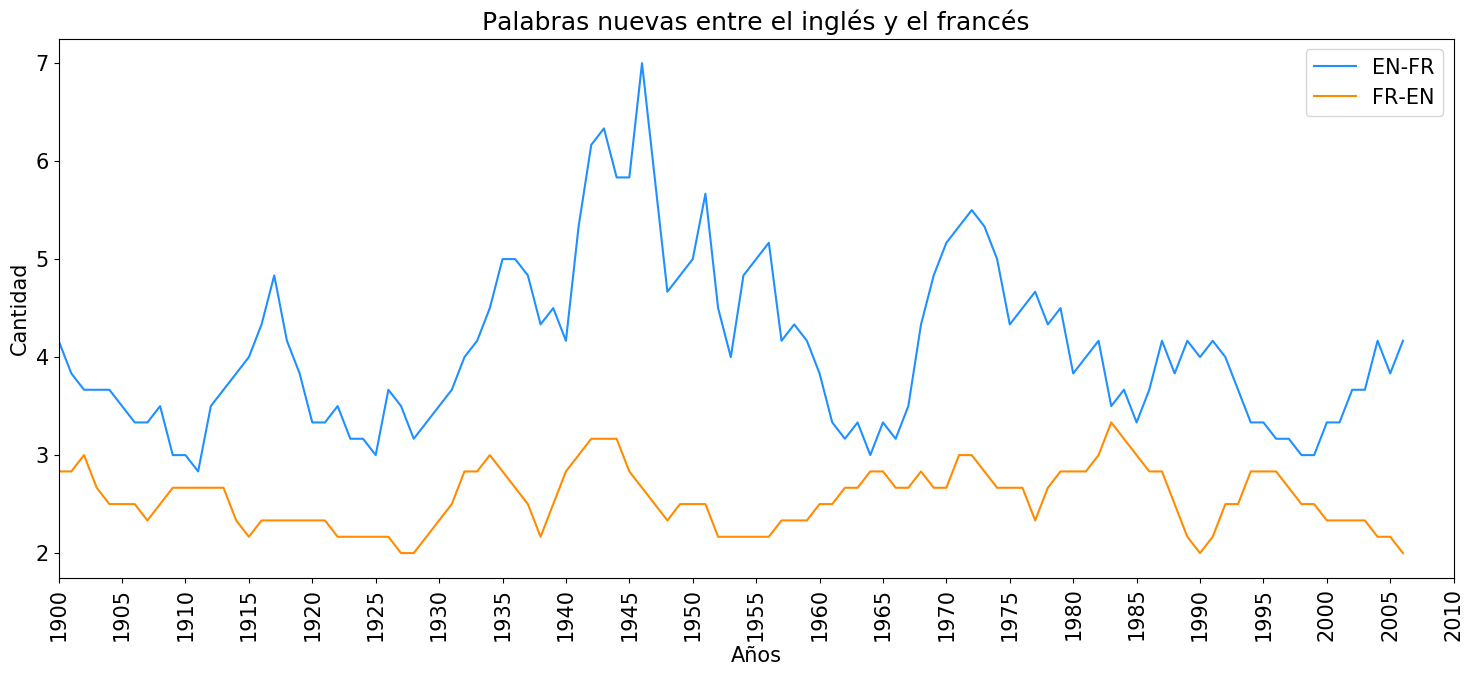
\includegraphics[scale=.38]{Cap_2/NC_1_S2_EN.png}
	\label{NC_EF}
	\caption{}
\end{figure}


La primera conclusión tras ver la gráfica, es que el inglés aportó mayor cantidad de palabras al francés que el caso contrario, los aportes no fueron constantes, sino que existieron períodos de tiempo 1910-1920, 1935-1960, 1965-1975 donde la migración fue más evidente (periodos donde hay picos en las trazas).  En el contexto histórico, en los primeros dos periodos ocurrieron las guerras mundiales, donde intervinieron países de habla inglesa y francesa.   Este argumento puede ser comprobado al consultar la lista de préstamos nuevos del inglés al francés; específicamente para los años 1944 y 1945, entre el contenido de la lista se encuentran \textit{Churchill}, \textit{territories,} \textit{nazis} y \textit{catastrophe} palabras que están relacionadas con la segunda guerra mundial por los años de aparición. Para el último periodo,  el contenido de la lista tiene palabras como \textit{Nixon} \textit{dollar} y \textit{Johnson}; dos de estas palabras aluden a apellidos que fueron importantes en el periodo, posiblemente ya existían estas palabras en el francés, pero hasta los años entre 1965 y 1975 fue que cobraron notoriedad por algún personaje que fue importante en esa época,  específicamente Lyndon B. Johnson y Richard Nixon, presidentes de Estados Unidos entre 1963-1969 y 1969-1974 respectivamente.

Los periodos más prolongados donde existieron aportes del francés al inglés,  ocurrieron entre 1930-1950 y 1975-1990,  sin embargo la lista de los préstamos no muestra palabras que se puedan asociar a un evento,   pero si hay palabras comunes en el inglés y el programa las detecto como provenientes del francés, como lo son \textit{diagnostic,} \textit{clients,} \textit{placement,} \textit{adaptation,} \textit{diffusion,} \textit{amplitude,} entre otras, estas son palabras que el programa clasificó como de origen francés, ya que fue el primer idioma donde tuvieron relevancia,  y que después las retomo el inglés. Esta propuesta puede sugerir que en años anteriores el francés era rico o basto de palabras de otros idiomas, o que los idiomas utilizaban al francés para poder llegar a más conjuntos. En un análisis posterior, se mostrará el uso que tenía el francés en el siglo XIX, comparado con el que tuvo en el siglo XX. 

De manera general para todos los idiomas, existirán casos donde las préstamos de un idioma en otro serán nombres, apellidos, ciudades o países, como el caso que ya se comentó anteriormente. Estas palabras pueden mostrar un evento histórico al estar relacionada con personajes o lugares del evento y también por la fecha en la que aparecieron. 


\newpage


\subsection{Inglés y Alemán}


\begin{figure}[h!]
	\centering
	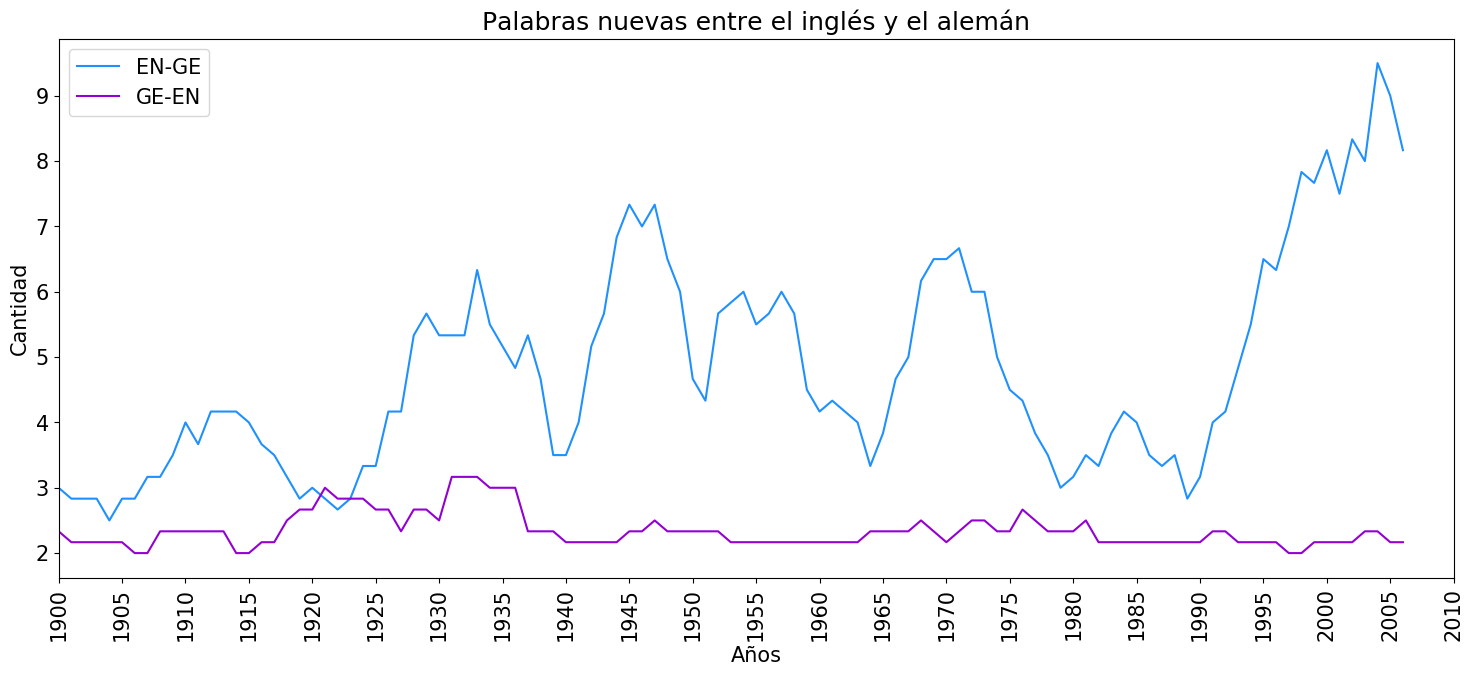
\includegraphics[scale=.38]{Cap_2/NC_2_S2_EN.png}
	\label{NC_EG}
	\caption{}
\end{figure}


El mayor aporte ocurrió del inglés al alemán, hay muchos periodos donde la cantidad de préstamos sobresalen, el primero entre 1920 y 1935,  el inglés aportó  palabras como \textit{economic} (1929), \textit{depression} (1931),  \textit{investment} (1933), \textit{Roosevelt} (1935) , que pertenecen al campo semántico de la gran depresión, evento que tuvo origen en los Estados Unidos  con consecuencias en muchos países, en este caso en Alemania, ya que fue uno de los motivos para que se originara la segunda guerra mundial.  Durante los años de la segunda guerra las palabras encontradas fueron \textit{Churchill} (1940), \textit{Stalin} (1943), \textit{nazi} (1945),  \textit{justice} (1947),  las cuales si están relacionadas con el suceso.  Finalmente alrededor de 1990, el inglés ha aportado de manera creciente más palabras al alemán, el desarrollo de la tecnología y la globalización son responsables de esta tendencia al estar involucradas palabras como \textit{standards} (1933), \textit{market} (1994),  \textit{internet} (1996), \textit{online} (1988). 

Para el préstamo en sentido inverso, el alemán presentó muchos años donde no llevó palabras de él hacia el inglés,  pero las pocas que lo hicieron muestran información histórica, como \textit{Lenin} (1931), \textit{Marx} y \textit{Hitler} (1934),  \textit{reich} (1939) y  \textit{Mao} (1967),  en alusión a la segunda guerra mundial y a la revolución china que ocurrió durante la guerra fría.

La relación entre el inglés y el alemán en el ámbito de préstamos se vio marcada por palabras que van de un lado a otro con relaciones a un hecho histórico que involucró a países cuyas lenguas son estos idiomas.  Por el momento se está haciendo evidente que los eventos políticos o históricos si permiten que exista una migración de palabras entre idiomas. 

\newpage
\subsection{Inglés e Italiano}

\begin{figure}[h!]
	\centering
	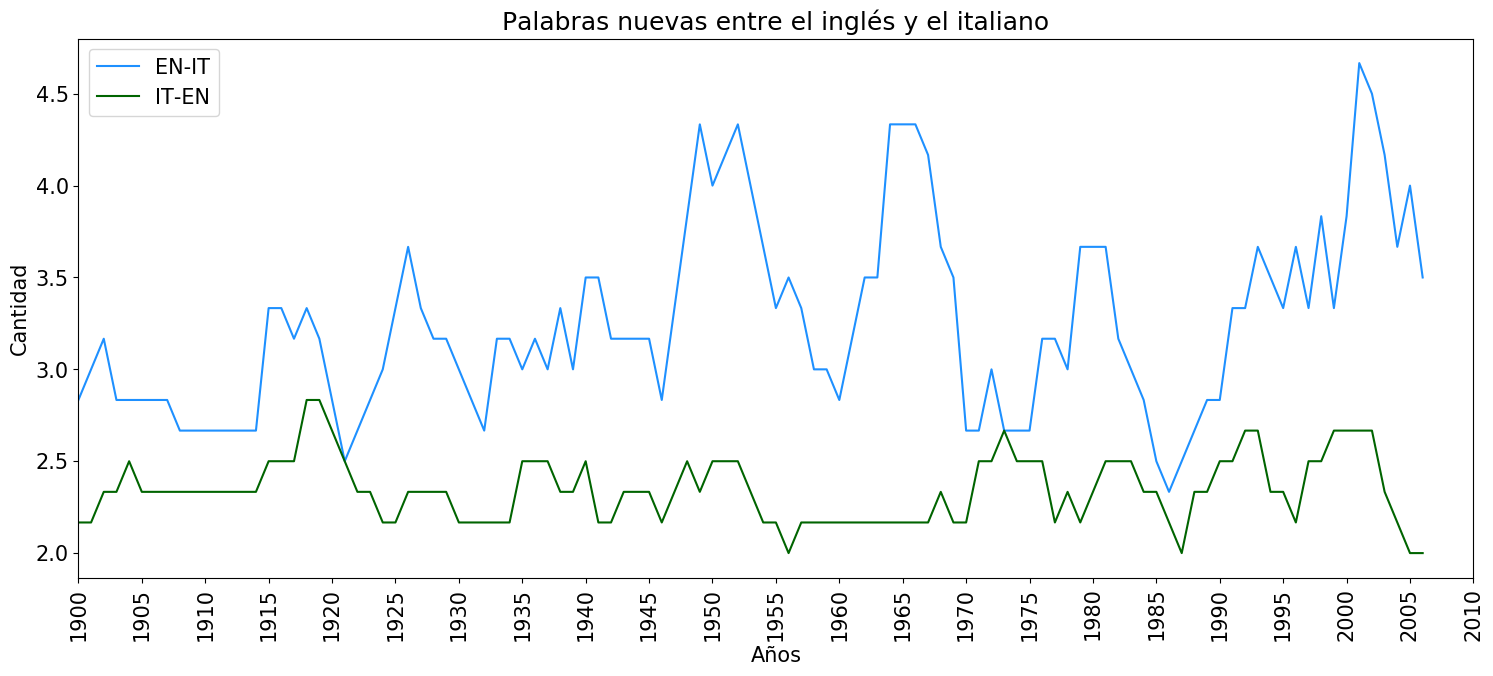
\includegraphics[scale=.38]{Cap_2/NC_3_S2_EN.png}
	\label{NC_EI}
	\caption{}
\end{figure}

El sentido de mayor cantidad de migraciones ocurrió del inglés hacia el italiano, donde es evidente periodos alrededor de las guerras como en el caso de las migraciones del inglés hacia el francés y el alemán,  nuevamente palabras como \textit{Roosevelt} (1941) o \textit{Stalin} (1949) son de carácter histórico; \textit{Mussolini} (1935)  presente en las migraciones del italiano al inglés es otro ejemplo de la relación de la guerra con estos idiomas y en esos años.A pesar de que la gráfica del inglés al italiano se vea favorecida en cantidad, muchas de las palabras no se consideraron préstamos de carácter histórico, ya que son palabras que no portan información que las ligue a un evento, sin embargo se asentaron en el italiano y han sido usadas en al menos dos años dentro de la lista de cinco mil. 

Los préstamos del italiano en el inglés, fueron nulos durante muchos años, los pocos en los que existieron, las palabras no se lograron  ligar a un suceso que explicara el por qué ocurrieron las migraciones,  salvo el ejemplo ya mencionado.

\newpage


\subsection{Inglés y Español}
\begin{figure}[h!]
	\centering
	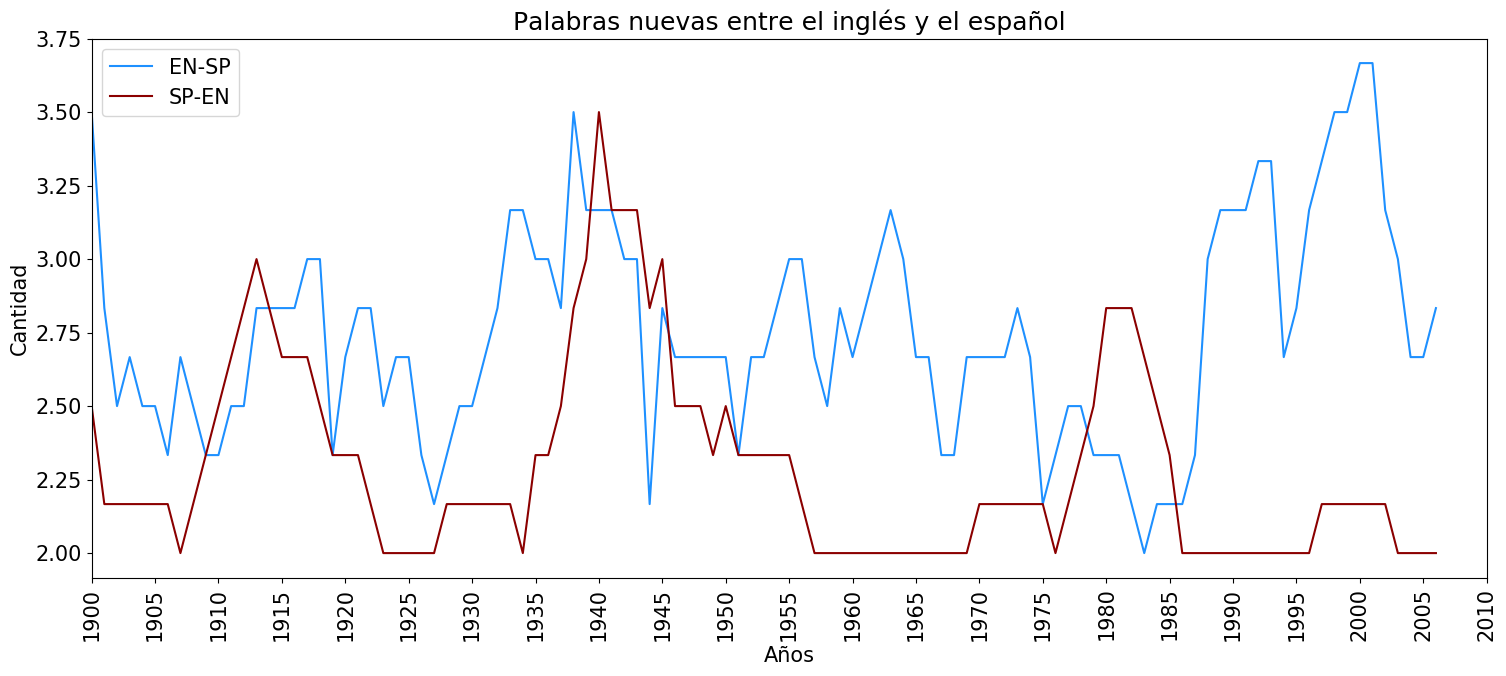
\includegraphics[scale=.38]{Cap_2/NC_4_S2_EN.png}
	\label{NC_ES}
	\caption{}
\end{figure}

El español ha sido el único idioma que ha aportado en algunas épocas igual cantidad de palabras al inglés como el inglés aportó al español,  en los demás idiomas la tendencia era que el inglés aportaba más que los demás a él.  Las dos gráficas muestran similar crecimiento en periodos de la primera mitad de siglo,  como de 1905 - 1925, y en 1935-1950.  En la segunda mitad del siglo XX,  se presentaron mayor cantidad de préstamos del inglés al español, y el sentido opuesto tuvo muchos periodos donde no aportó alguna palabra,  siendo el más relevante entre 1975 y 1985. 

Entre los préstamos encontrados en el sentido inglés-español, se encuentran \textit{oil} (1931), \textit{standard} (1933),  referentes a la compañía de petróleos de Standart Oil de John D.  Rockefeller,  \textit{unesco} (1955); de estas palabras es curioso que aparecieron en el español tras un letargo de años en el que eran importantes en el inglés,  por ejemplo, la empresa Standard Oil, cobró relevancia por ser el primer gran monopolio entre finales del siglo XIX y su disolución en 1911,  transcurrieron cerca de treinta años para que el español se comenzará a hablar acerca de ello. Un letargo menos extenso ocurrió con la palabra Unesco, esta organización se fundó diez años antes (1945)  de que entrara a la lista de español.  

Conforme se avanza en los años, aparecen palabras como \textit{Kennedy} (1961), \textit{nuclear} (1962) (sin acento al provenir del ingles), \textit{Nixon} (1972),  \textit{Bush} (1990), \textit{internet} (1996) e  \textit{Irak} (2003),  de este conjunto, tres son apellidos de presidentes de los Estados Unidos, pero no hay un desfase prolongado entre la fecha de relevancia en el conjunto original (para este caso los años en que fueron presidentes) y el año donde aparecen en el receptor. Palabras como nuclear e Irak, también son de carácter histórico aludiendo a los conflictos bélicos que se dieron alrededor de su fecha de aparición, igualmente no tuvieron un desfase de años, mientras que internet alude al desarrollo de esta herramienta. 


Por parte de los préstamos que van del español hacia el inglés,  se lograron ligar palabras al campo de la medicina,  en el año de 1943 aparecieron las palabras \textit{virus} y \textit{anemia}, años antes en 1934 George Richards Minot, Parry Murphy y George Hoiyt Whipple, habían recibido el premio nobel de medicina por su descubrimiento de la terapia de hígado en las anemias.  También migraron nombres de países como \textit{Chile} (1920), \textit{Argentina} (1941),  \textit{Venezuela} (1942).

La conclusión general  de estos argumentos es que la “velocidad” con la que se transmiten palabras de un idioma a otro,  ha ido en aumento conforme se avanza en el tiempo, permitiendo que cada vez sea más inmediata, además las palabras ligadas a sucesos históricos no son solo en el ámbito político, sino también al desarrollo científico y tecnológico. 


\hfill\break

\subsection{Francés y Alemán}

\begin{figure}[h!]
	\centering
	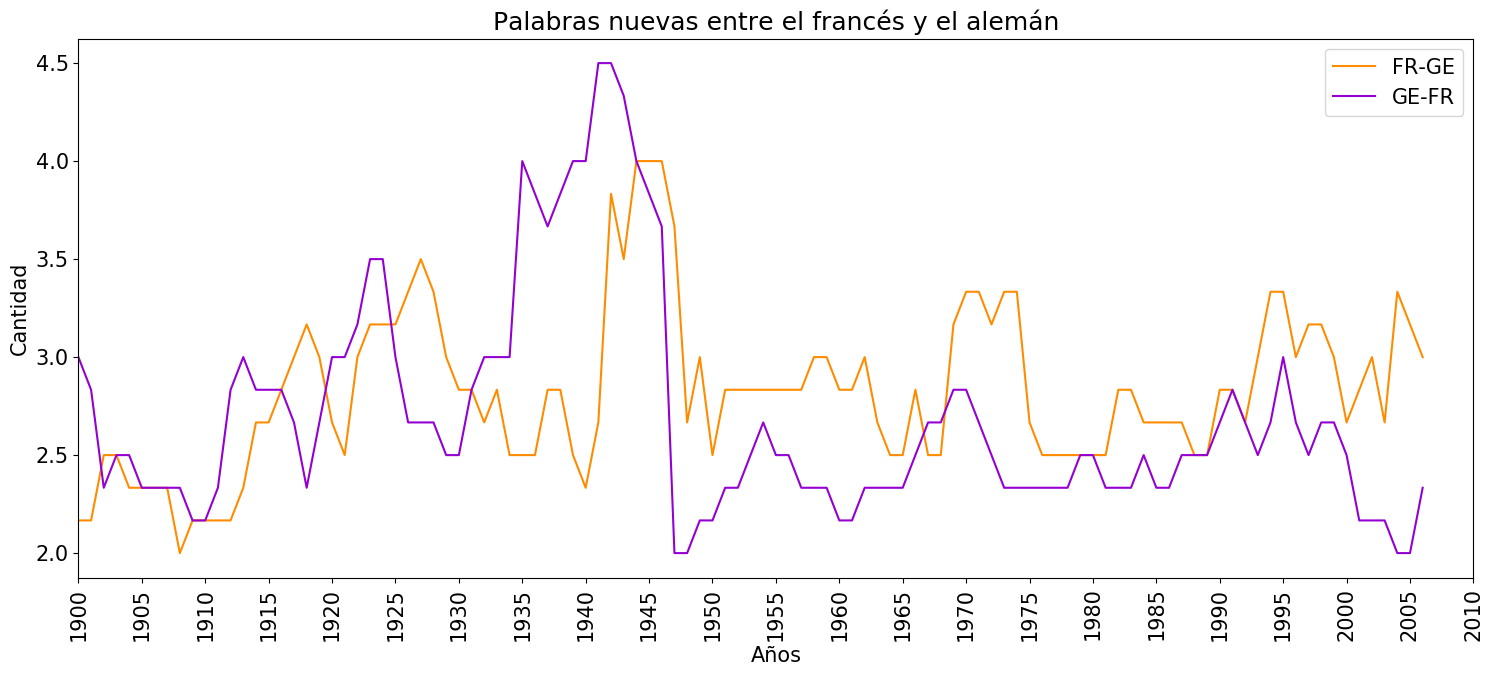
\includegraphics[scale=.38]{Cap_2/NC_2_S2_FR.png}
	\label{NC_FG}
	\caption{}
\end{figure}


Las aportaciones entre ambos idiomas han sido equitativas,  teniendo un comportamiento similar en diferentes plazos, el alemán logra su punto más alto entre 1940, mientras que el francés lo hace  en 1945.  Las primeras dos clafisicaciones que se hicieron para los préstamos que van del francés al alemán son a partir de términos políticos como \textit{diplomatie} (1917), \textit{bourgeoisie} (1919),  \textit{guerre} (1925),  \textit{empire} (1937), y por nombres de  países como \textit{Ukraine} (1918),  \textit{Allemagne} y \textit{Russie} (1925) y \textit{Vietnam} (1965).  Dentro de un entorno histórico,  ambas clasificaciones pueden simplificarse en una, ya que para los años de aparición, es posible que en una misma oración o párrafo coexistan palabras de las dos clasificaciones.  La última clasificación hecha para esté sentido de migración son términos del campo semántico del desarrollo tecnológico como \textit{technologie} (1969),  \textit{innovation} (1996), \textit{informations} (1997),  \textit{mobile} y \textit{communication} (2007).  Estas palabras también tienen en común que su origen es el inglés y que aparecieron en la segunda mitad de siglo, posiblemente gracias a la globalización. 

Para la gráfica de las palabras que parten del alemán hacia el francés, el punto más alto se logró alrededor de 1944,  dentro del contenido para esté año se encuentran  \textit{regierung},  \textit{deutschen},\textit{minister} y  \textit{bestimmungen} (traducciones de gobierno, alemán, ministro y reglamentos);   si se añaden palabras en años previos como \textit{Hitler} (1933),  \textit{tirailleurs} (1931),  e incluso \textit{kaiser} (1915) y \textit{reich} (1921), son conceptos que muestran parte de la historia bélica que vivieron los hablantes del alemán, hechos de gran importancia que fueron adoptados por los francoparlantes. 

El objetivo no es solo identificar sucesos de carácter militar en esta dirección de los préstamos, el identificar un nombre o apellido facilita encontrar las relaciones con un ámbito,  además de Hitler se encontralos los siguientes apellidos:  \textit{Nietzsche} (1905),  \textit{Marx} (1923), \textit{Heidegger} (1987),  \textit{Mozart} (1956), \textit{Freud} (1965) y \textit{Engels} (1970), enlazados a la filosofía, la música y la medicina,  además todos ellos de personajes nacidos en países germanohablantes.


\newpage

\subsection{Francés e Italiano}

\begin{figure}[h!]
	\centering
	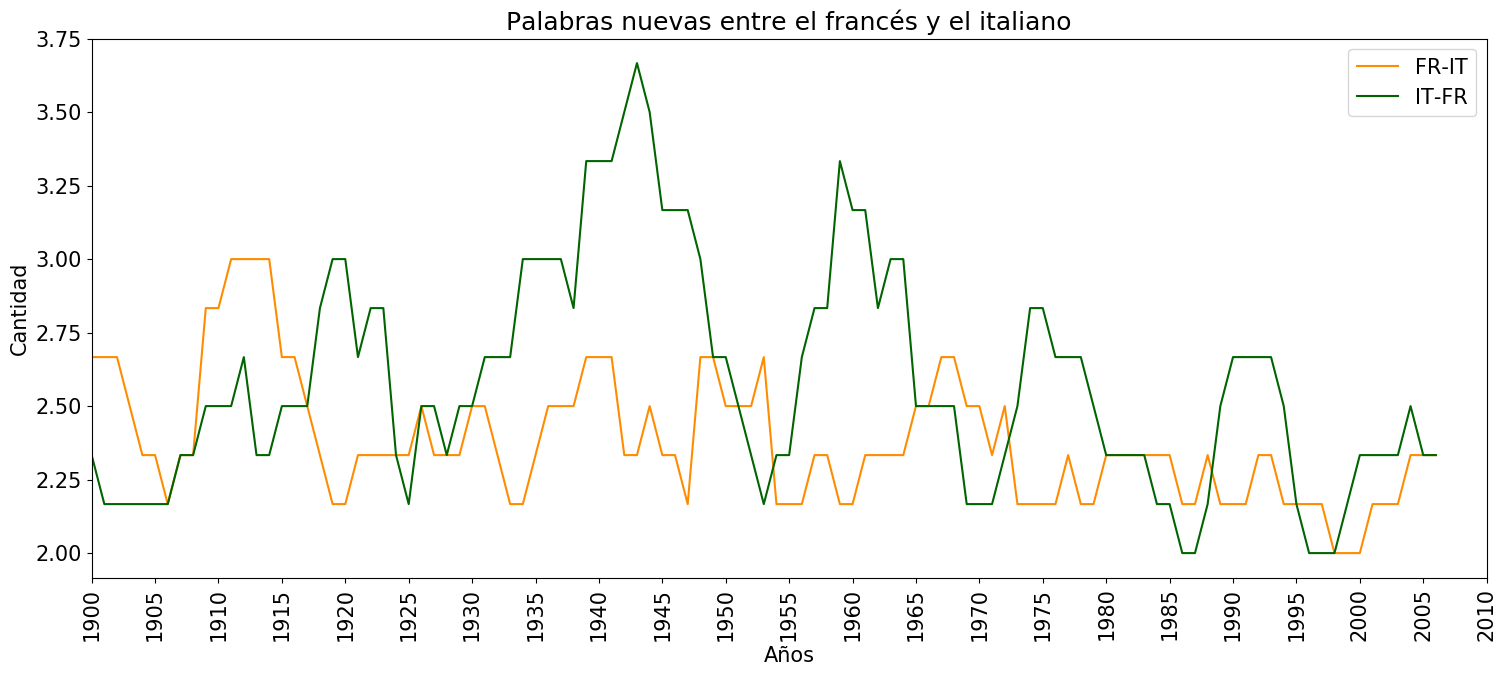
\includegraphics[scale=.38]{Cap_2/NC_3_S2_FR.png}
	\label{NC_FI}
	\caption{}
\end{figure}

La mayoría de los préstamos que ocurrieron entre estos idiomas provienen del italiano como el idioma origen, logrando puntos contrastantes con las migraciones provenientes del francés. Aunque países como Italia y Francia  fueron relevantes durante los años del análisis,  la mayoría de las palabras encontradas no brindan información para familiarizar a algún hecho,  en las pocas que se lograron conectar del francés al italiano están \textit{Versailles} y \textit{Poincaré} (1924) aludiendo al tratado de paz de la primera guerra mundial y al matemático francés.  También se encontró  \textit{Vietnam} (1966) y \textit{URSS} (1975), aunque no son términos franceses, si fue el francés el primero en hablar de ellos e importarlos a los demás idiomas.

En las migraciones con origen en el italiano, se encuentra \textit{Mussolini} (1935), la cual ya se había mencionado en las migraciones del italiano al inglés, tras revisar las listas de migraciones con origen italiano  a los demás idiomas, Mussolini siempre se encuentra en la lista de préstamos y con el mismo año de aparición en los demás idiomas.  Aunque solo sea una palabra, el estar en todos los idiomas del análisis ejemplifica la importancia de la misma en el siglo XX. 

\newpage
\subsection{Francés y Español}

\begin{figure}[h!]
	\centering
	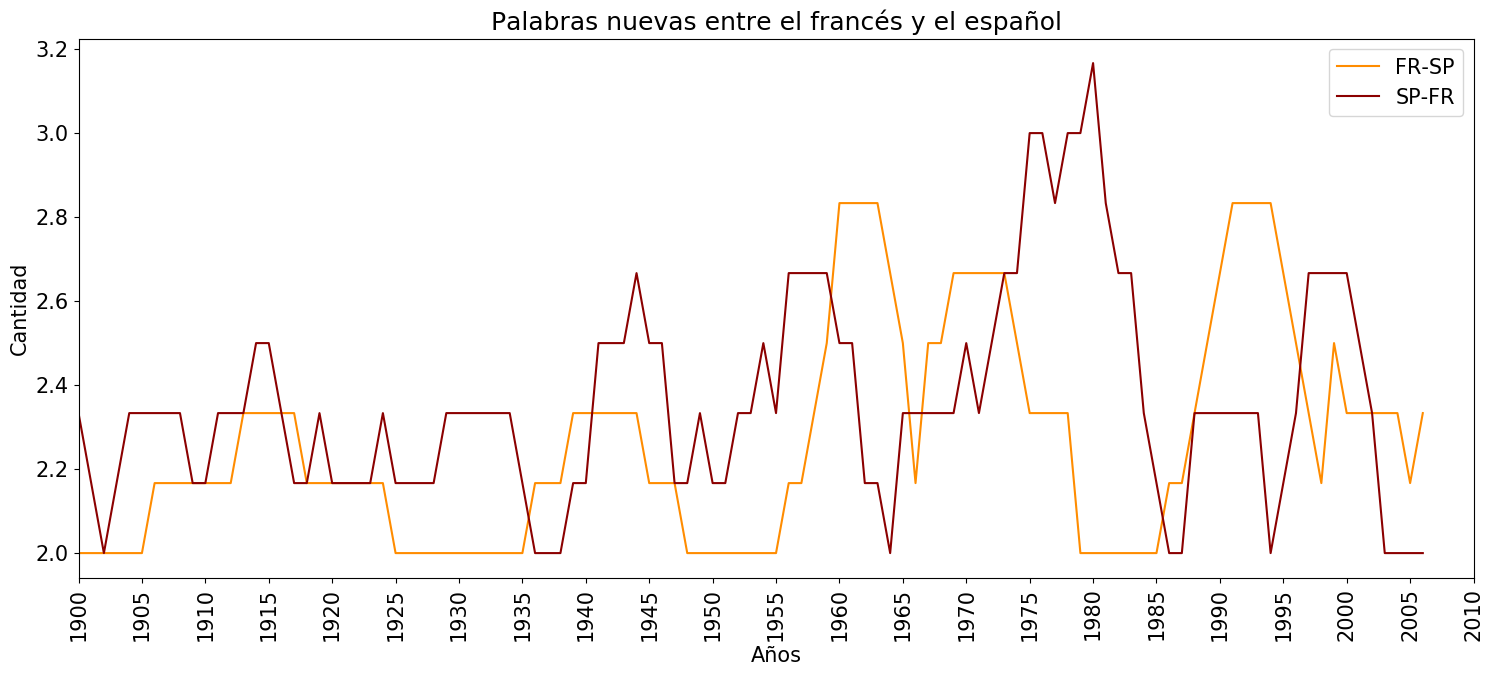
\includegraphics[scale=.38]{Cap_2/NC_4_S2_FR.png}
	\label{NC_FS}
	\caption{}
\end{figure}

La tendencia de los préstamos del español hacia el francés presentó pocos años donde la cantidad de ellos fue nula, en comparación con los del francés al español donde se aprecian periodos sin una migración.  Por parte de los préstamos con origen en el francés y receptor hay una ausencia de palabras que representen información de la época, la más relevante es \textit{euros}, referente a la moneda de la Unión Europea, ya que el año de aparición en el español y el año en el que empezó a circular de forma oficial coinciden, siendo el 2002.  La palabra \textit{ONU} (1995)  también se detectó en este sentido de migración; a pesar de ser la abreviación de  una organización mundial,  a la cual no se le puede asignar el francés como idioma origen, pero sí fue el francés el primer idioma ( entre los idiomas del trabajo)  en hablar de ella, y aunque la ONU tenga al español como uno de sus seis idiomas oficiales,  dentro de las publicaciones en español, la palabra ONU entró a la lista de las cinco mil más usadas  cincuenta años después de su fundación en 1945. Otras palabras encontradas son \textit{URSS} (1962) y  \textit{Vietnam} (1965),  las cuáles ya se habían mencionado en las anteriores migraciones del francés. 

El primer préstamo que resultó importante del español hacia el francés es \textit{Panamá}\,\,\, (1913), su trascendencia se liga al año de inauguración del canal de Panamá en 1914, siendo la obra una de las más importantes para el comercio de la época al conectar los océanos pacífico y atlántico, además el primer gobierno que impulsó económicamente la construcción del canal fue el francés,  aunque su conclusión y administración pasó a los Estados Unidos.  Las demás palabras incluidas las que migraron entre 1965 y 1985 no se logró identificar su relación con suceso  en el cual hayan sido importantes.

\hfill\break
\subsection{Alemán e Italiano}

\begin{figure}[h!]
	\centering
	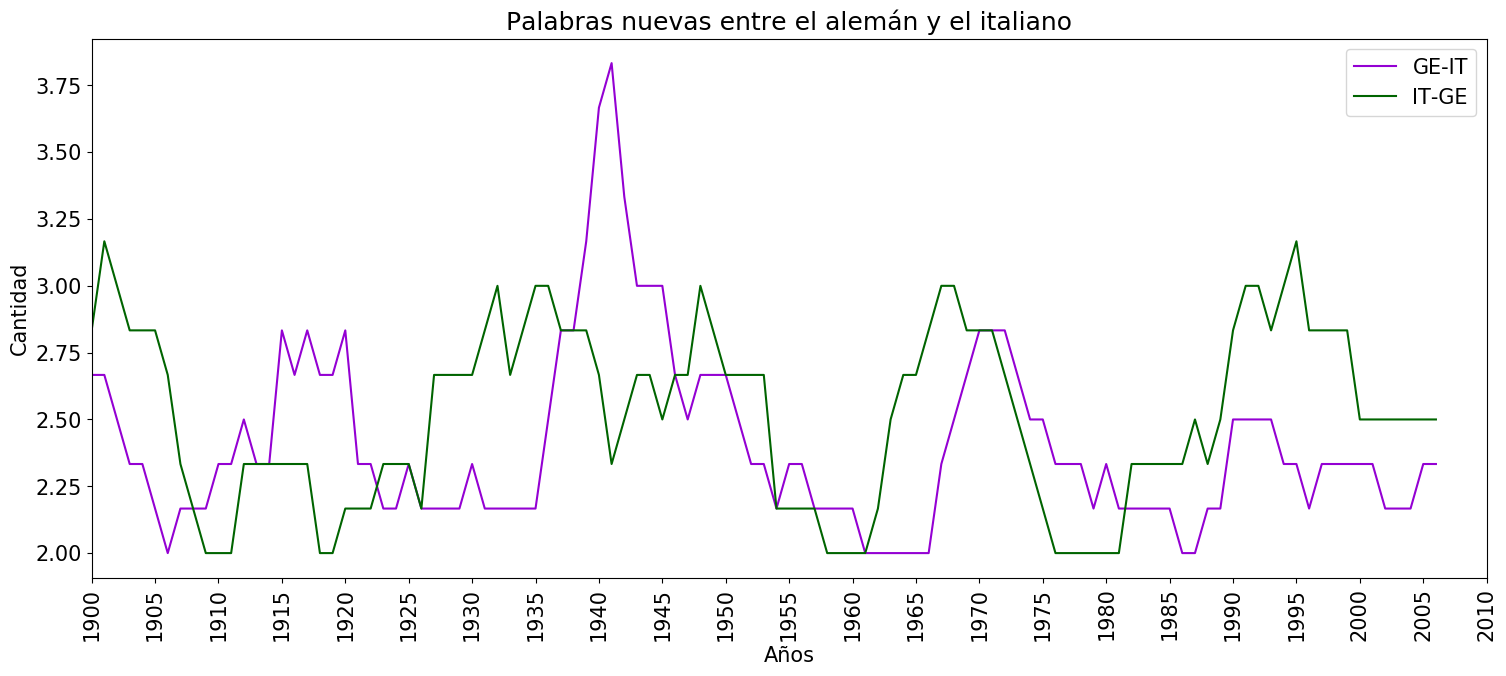
\includegraphics[scale=.38]{Cap_2/NC_3_S2_GE.png}
	\label{NC_GI}
	\caption{}
\end{figure}

La tendencia de las migraciones de palabras entre ambos idiomas se ve equitativa entre ambos idiomas,  siendo el punto más destacado alrededor de 1940 por parte del alemán como idioma origen. 

Tras la revisión de los préstamos del alemán hacia el inglés y el francés, se han destacado apellidos de personajes germano hablantes que destacaron en alguna disciplina. El apellido que se asentaron únicamente en el  italiano fue \textit{Berchtold} en 1943,  un año después de la muerte Leopold Berchtold (21 de noviembre de 1942) ministro de exteriores del Imperio Austro-Húngaro de 1912 a 1915, fecha coincidente con el inicio de la primera guerra mundial.  La relación entre la palabra y la fecha con los dos idiomas se puede explicar por las relaciones que tuvieron el imperio Austro-Húngaro con Italia, y además la parte germano parlante del imperio (actualmente Austria) tenía  fronteras con Italia, sumado a que una de las consecuencias de la primera guerra mundial fue la disolución del Imperio.  El argumento de las fronteras físicas entre países con diferentes idiomas oficiales, ejemplifica una de las posibles causas de la migración de palabras entre idiomas, ya que el intercambio cultural  y las relaciones entre ambas naciones pueden ser más activas o dinámicas permitiendo un mayor flujo de términos. 

Los préstamos del Italiano al Alemán permitieron relacionar con contextos bélicos de la época de la segunda guerra mundial a \textit{regime} (1938), \textit{panzer} (1941), \textit{duce} (1942),  traducciones de régimen, blindado y líder, además de \textit{Mussolini} (1935).  Uno de los errores que se encontró fue la palabra \textit{Franco} (1951), que por la fecha hace referencia al dictador español Francisco Franco; al ser un apellido, se registró como origen Italiano, pero mostrando como un término que es popular en un idioma diferente al origen, emigra a los demás idiomas  por un conjunto auxiliar.


\subsection{Alemán y Español}

\begin{figure}[h!]
	\centering
	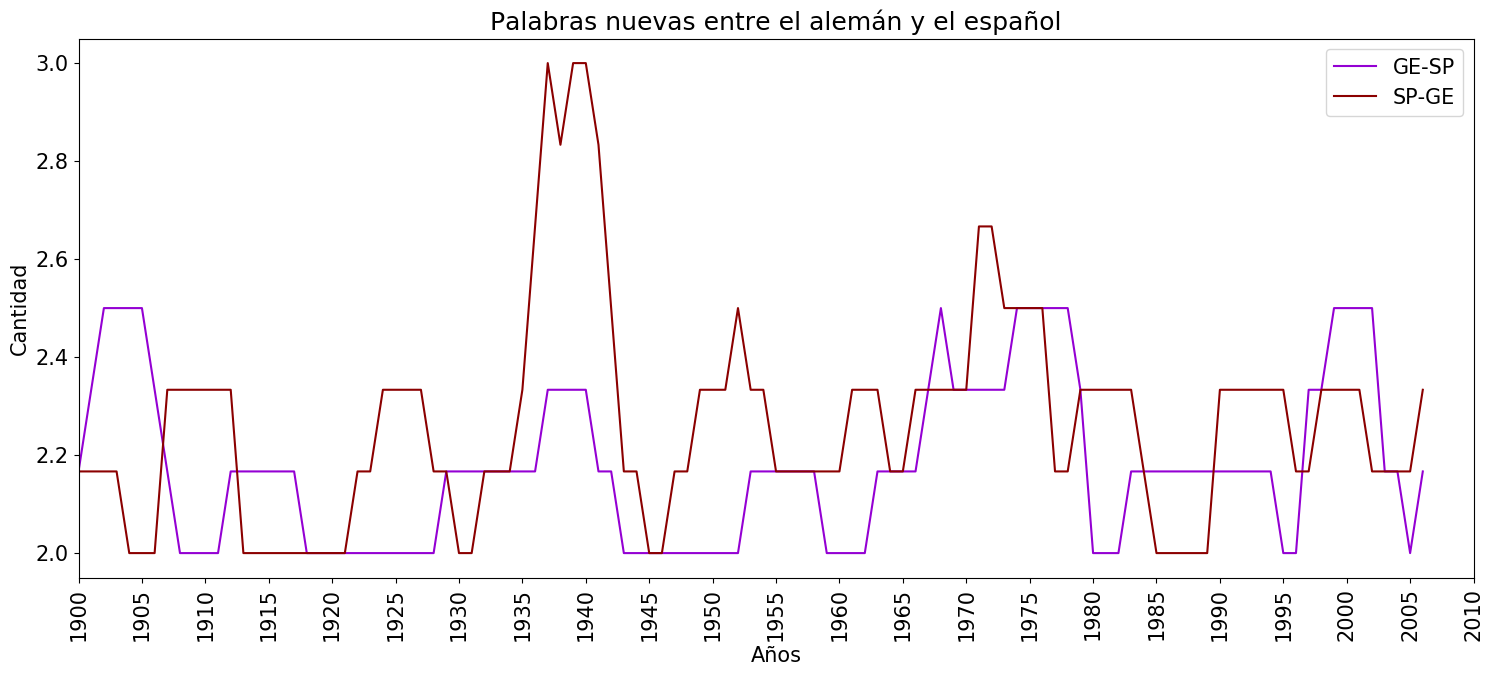
\includegraphics[scale=.38]{Cap_2/NC_4_S2_GE.png}
	\label{NC_GS}
	\caption{}
\end{figure}

La diferencia más marcada en las gráficas corresponde a las migraciones del español hacia el alemán entre 1930 y 1945, fechas que coinciden con el desarrollo de la segunda guerra mundial, sin embargo no se encontraron palabras que se relacionen con el evento.  La investigación hecha para ligar las palabras del español hacia el alemán con sucesos, muestra que la palabra \textit{lepra} (1901) fue globalmente importante a partir de 1874,  ya que en ese año el científico noruego Gerhard Armauer Hansen descubrió el bacilo de Hansen Mycobacterium Leprae \cite{lepra} que origina la enfermedad,  por el carácter médico de la palabra es probable que se hiciera más investigación sobre la enfermedad en diferentes idiomas, en este caso el alemán,  tras el descubrimiento del bacilo.  Este es otro caso de una palabra que se origina en un idioma (español), pierde  relevancia al transcurrir los años y tras un suceso (el descubrimiento del bacilo)  retoma importancia y migra a los demás idiomas (alemán).   Entre las otras palabras que pasaron al alemán están \textit{virus} (1939) que ya se ha tratado en los préstamos del español al inglés, \textit{China} (1955) referente al país y su relevancia en la segunda mitad del siglo XX por la revolución China de 1949, e \textit{India} (1970) igualmente se conecta con el país ya que en 1965 ocurrió la guerra indo-pakistaní,  también en 1968 hubo una extensa cobertura mediática a la banda británica The Beatles que visitó el norte de la India para meditar.

Las palabras que van en el sentido alemán-español,  presentaron muchos años sin una migración, el incremento de ellos se dio posterior a 1950  donde los años sin intercambio disminuyeron. En el contenido de la lista se encuentran palabras que ya se han tratado como \textit{Marx} (1932), \textit{kaiser} (1938), \textit{Hitler} (1940), \textit{Lenin} (1970), \textit{Hegel} (1971),  \textit{Nietzsche} (2000) y \textit{Freud} (2002).  Es peculiar que las dos últimas hayan aparecido en el español muchos años después que en los demás idiomas, por ejemplo en el francés Nietzsche apareció 1905 y Freud en 1965. El letargo de años puede ser una característica de el tiempo que les lleva  a las  palabras de un idioma  pasar hacia el español,  sobretodo si son palabras con un origen antiguo.

\hfill\break
\subsection{Italiano y Español}

\begin{figure}[h!]
	\centering
	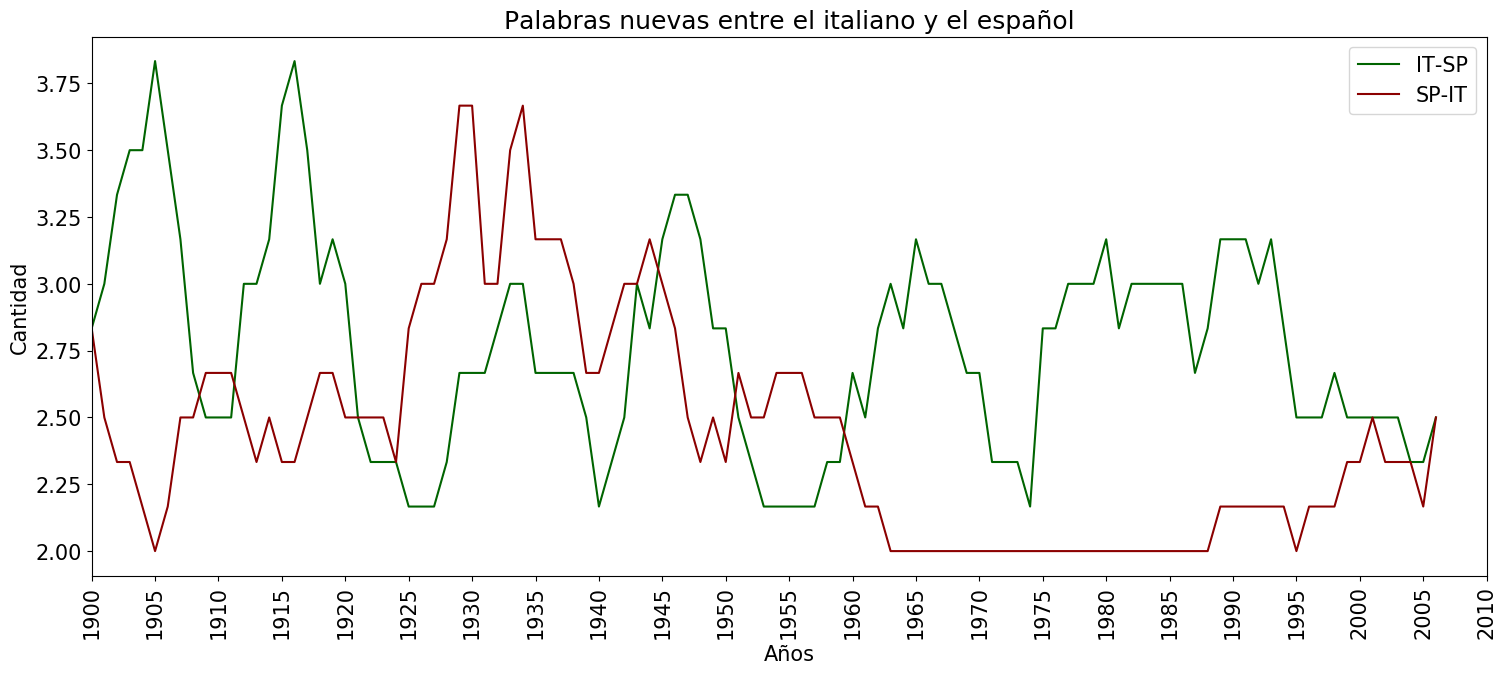
\includegraphics[scale=.38]{Cap_2/NC_4_S2_IT.png}
	\label{NC_IS}
	\caption{}
\end{figure}

Entre estos idiomas se dio la mayor cantidad de intercambios de palabras durante el siglo XX, durante la primera mitad, las aportaciones fueron equitativas con dos periodos donde dominó el italiano y dos donde dominó el español; a partir de 1960 el dominio fue italiano, ya que los aportes del español  fueron nulos hasta 1900. 

Por parte de los préstamos del italiano al español, se encuentran muchos con tendencias hacia ideologías políticas como \textit{socialista} (1914), \textit{comunista} (1932), \textit{capitalismo} (1935), \textit{fascismo} (1937),  \textit{marxismo} (1963) y \textit{terrorismo} (1986), palabras que por las fechas fueron importantes no solo en el italiano y el español, sino globalmente, ya que estas ideologías repercutieron en eventos como la guerra fría y la economía.  Una palabra que no se había tratado es realismo (1948) que tuvo un impulso por la corriente literaria del realismo mágico originado en varios países de Latinoamérica, cuyas obras trascendieron en la literatura. 

En las palabras que se originan en el español y llegan al italiano, se encontró \textit{idealismo} (1920) otra ideología política,  y palabras de términos médicos como \textit{virus} (1922), \textit{colesterina} (1928),  \textit{sintomatología} (1931), \textit{anestesia} (1932), \textit{vitamina} (1935), \textit{anemia}, \textit{metabolismo} y \textit{gástrica} en 1936  y \textit{endovenosa} (1937).  Este grupo de términos apareció en un periodo de veinte años, probablemente por la publicación de un texto que se popularizó, ya que muchas de estas palabras tienen su traducción al italiano. En los demás años, no se encontraron más palabras con un tema común al cual relacionar. 

\hfill\break
\hfill\break
\hfill\break
\section{Conclusiones del método}

El método de buscar préstamos nuevos mostró el diverso contenido de los préstamos que se lograron asociar un hecho,  por parte del inglés, las mayores aportaciones fueron apellidos de los presidentes de los Estados Unidos, y por el papel que tuvo este país en diferentes campos como la economía, la ideología política, el desarrollo industrial, la globalización y su participación en las grandes guerras, logró que sus jefes de estado fuesen relevantes en cada ámbito que se suscitó en la época que gobernaron.  Por parte del inglés como idioma receptor,  las palabras que emigraron al inglés, no exhibieron una tendencia clara sobre el campo al cual relacionarlas,  muchas de ellas son palabras con origen etimológico en el inglés pero que fueron más relevantes  en otros idiomas, antes de tomarlas como un error, estas palabras muestran que antes del siglo XX el inglés no tenía la importancia que actualmente posee, y que se apoyaba en otros idiomas para que sus vocablos fuesen conocidos. 

El Alemán fue otro conjunto donde los préstamos que llegan a otros idiomas se caracterizan por ser apellidos de personajes, a diferencia del inglés, los campos donde destacaron los germanoparlantes fueron ciencias, filosofía, medicina y  por la historia de alemania en las guerras mundiales,  palabras de carácter bélico también migraron a los distintos receptores.

El francés, aportó endónimos a los otros idiomas, principalmente en las primeras décadas del siglo, reflejando la importancia que tuvo este idioma en el siglo XIX y principios del XX, al migrar palabras que tienen su propio significado y escritura en los demás idiomas.  Además de endónimos,  una porción significativa de los aportes son palabras etimológicas del inglés,  este punto ya fue discutido, pero es otra muestra de la relación que ha mantenido el inglés y el francés  desde antes de 1800, al tener el inglés muchas palabras provenientes de la familia del francés, es decir las lenguas grecolatinas. 

El italiano migró términos políticos a los demás idiomas, principalmente al español,  mientras que el español fue diverso en el contenido de sus préstamos,  desde expresiones médicas, nombres de países y  literatura. La diversidad del español se puede deber a la cantidad de países donde es un idioma oficial,  y hay muchos elementos de diferentes culturas que se exportan a los demás idiomas. 

Tanto el francés, el alemán, el italiano y el español,  se comportaron más como idiomas receptores que como portadores,  donde la mayoría de palabras provienen del inglés.  Entonces en términos de cantidad, el inglés ha sido el idioma que más ha influenciado a los demás, por los vocablos nuevos que de él han llegado.  


En términos de préstamos nuevos,  la influencia por cantidad mostró información histórica de los países en el siglo pasado,  pero no el cómo afectan las nuevas palabras a los idiomas receptores. Si los préstamos nuevos cobran relevancia en el idioma receptor, el rango que ocupan disminuye en cada lista tras el año en que se localizaron,  sin embargo se encontraron años donde no hay préstamos nuevos, y al ser pocos en comparación a las cinco mil palabras, su frecuencia de uso, ecuación \ref{ec.fuso} es casi nula, por ello la mejor forma de utilizar a la frecuencia de uso es usando el background de préstamos acumulados. 
















	
%\include{Capitulo2/marco_teorico}           % ~20 páginas - Poner un contexto a la tesis, hacer referencia a trabajos actuales en el tema
\chapter{Análisis de acumuladas}

El objetivo sigue siendo determinar cómo influye un idioma en otro,  y el analizar los préstamos nuevos no brindó información de las palabras que para 1900 ya formaban parte de los idiomas y que provenían de algún otro, es por ello que se ha decidido emplear a los préstamos acumulados.  

La simbología para las gráficas es la misma de la sección anterior, manteniendo las abreviaciones, los colores y el significado de las leyendas.  Nuevamente en el eje horizontal se localizan los años  entre 1900 y 2008, y en el eje vertical la frecuencia de uso; la gráfica resultante se nombrará como gráfica de uso del idioma A en el idioma B. 

Para ciertas combinaciones de idioma origen e idioma receptor, se han localizado más de cien palabras que conforman los préstamos del origen que se han acumulado en el receptor, ya que la búsqueda se realiza en cada año, el proceso de analizar palabra por palabra (como en los préstamos nuevos) y tratar de ligar a un evento histórico es inviable. La forma en que se presentarán los resultados es la misma que en el análisis de préstamos nuevos,  mostrando las gráficas de uso de A sobre B y la B sobre A; el hacer esto permitirá ver si hay cambios en las tendencias de las gráficas y si se presentan cruces de ellas.

\newpage
\section{Palabras acumuladas entre dos idiomas}

\subsection{Inglés y Francés}

\begin{figure}[h!]
	\centering
	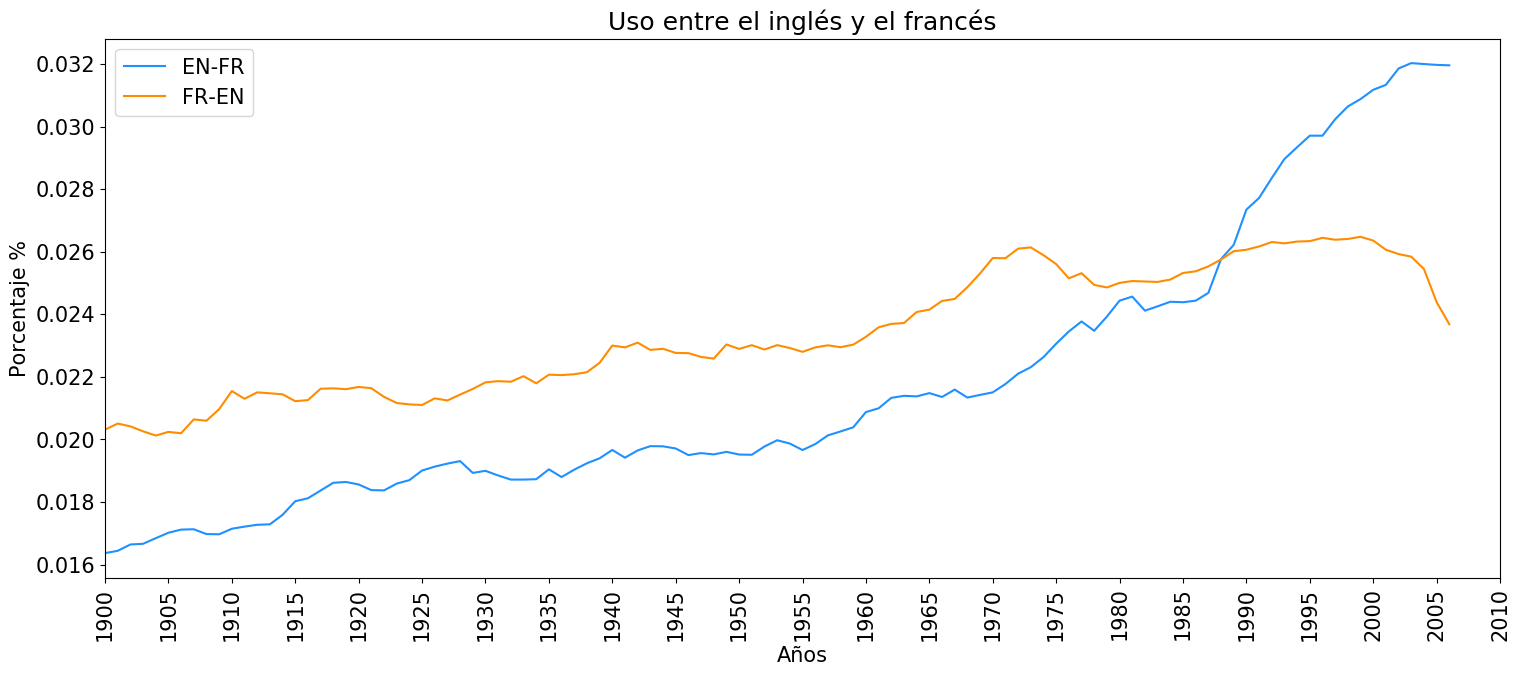
\includegraphics[scale=.38]{Cap_3/SF_1_S2_EN.png}
	\label{SF_EF}
	\caption{}
\end{figure}

Las gráficas de uso en ambos sentidos de los préstamos muestran una tendencia creciente desde el comienzo de las mediciones,  dominando el uso del francés en el inglés hasta 1990 donde se da el cruce de las gráficas para posteriormente ser los préstamos del inglés en el francés más utilizados que los de su contraparte.  A partir del cruce, es decir en los últimos veinticinco años, el inglés toma el lugar como idioma predominante despegándose en cada año que transcurre. 

Dentro de las palabras del inglés al francés que se han encontrado a partir del cruce en 1990 se encuentran internet, dollar, computer, communications, message, production;  palabras del campo semántico de la economía y la tecnología, disciplinas que se han favorecido una de la otra en los últimos años, y que han impulsado al inglés como un idioma común para la comunicación entre personas.  Otras palabras relevantes son Oxford y Cambridge,  ya que la extracción de palabras se obtuvo de los libros,  estas palabras muestran a ambas instituciones como líderes de editoriales, al ser los únicos nombres de editoriales en las listas.                         

El uso de los préstamos del francés en el inglés comenzó  a decaer tras el cruce siendo más evidente a partir del año 2000. Al analizar la lista de los préstamos, no hay cambios en las palabras que son más comunes por lo que a pesar de tener una palabra el mismo rango en las listas posteriores a la del año 2000,  su frecuencia disminuyó conforme transcurrieron los años; de forma generalizada el francés perdió importancia en el inglés en la primera década del siglo XXI.


\newpage
\subsection{Inglés y Alemán}

\begin{figure}[h!]
	\centering
	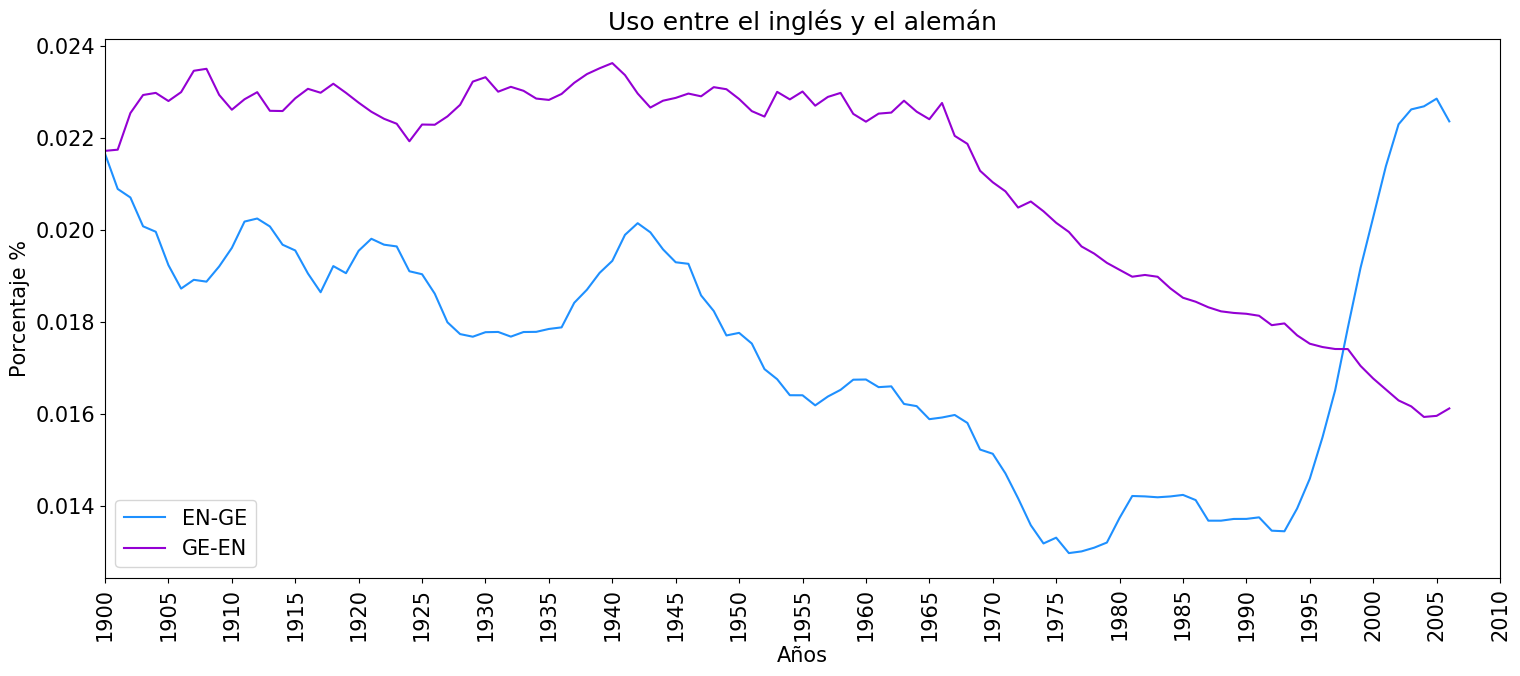
\includegraphics[scale=.38]{Cap_3/SF_2_S2_EN.png}
	\label{SF_EG}
	\caption{}
\end{figure}

En 1900 ambos idiomas eran igual de utilizados en el otro, pero al transcurrir el tiempo, las palabras del inglés comenzaron a ser menos utilizadas en los textos de alemán hasta alcanzar un mínimo de uso en 1990.  Al igual que en el francés, el aumento del inglés en el alemán comenzó a crecer después de 1990,  históricamente un año después de la caída del muro de Berlín, uno de los sucesos finales de los conflictos bélicos del siglo XX donde estuvieron involucrados países hablantes de ambas lenguas. La lista de préstamos acumulados muestra que las palabras ligadas a tales conflictos y que se catalogaron dentro de los préstamos nuevos de la sección anterior, están presentes en los años donde aumenta el uso del inglés en el alemán y continúan hasta el último año del análisis. Parte del gran crecimiento (de 0.014$\%$ a 0.024 $\%$) del inglés se asocia a la historia que compartieron ambos idiomas,  además los términos que involucran a la globalización como internet, mail, online, windows, marketing, financial, donde nuevamente los países hablantes de inglés o alemán han sido referentes en el desarrollo  científico y tecnológico de la primera década del dos mil.

El uso  del alemán en el inglés  se mantuvo en un umbral alrededor del 0.023 $\%$  por un periodo de casi sesenta y cinco años tras el cual comenzó su declive. Uno de los motivos de la pérdida del descenso en el uso es la situación que vivieron los países germanófonos en los años posteriores al término de la segunda guerra mundial,  donde la ideología política, la economía, los cambios territoriales y la intervención extranjera altera al idioma haciéndolo susceptible y debilitando su influencia ante los demás.  Este razonamiento puede ser arriesgado, sin embargo se planteará un algoritmo para decir en cual momento los idiomas son más propensos a perder  o ganar influencia en los demás.


\newpage
\subsection{Inglés e Italiano}

\begin{figure}[h!]
	\centering
	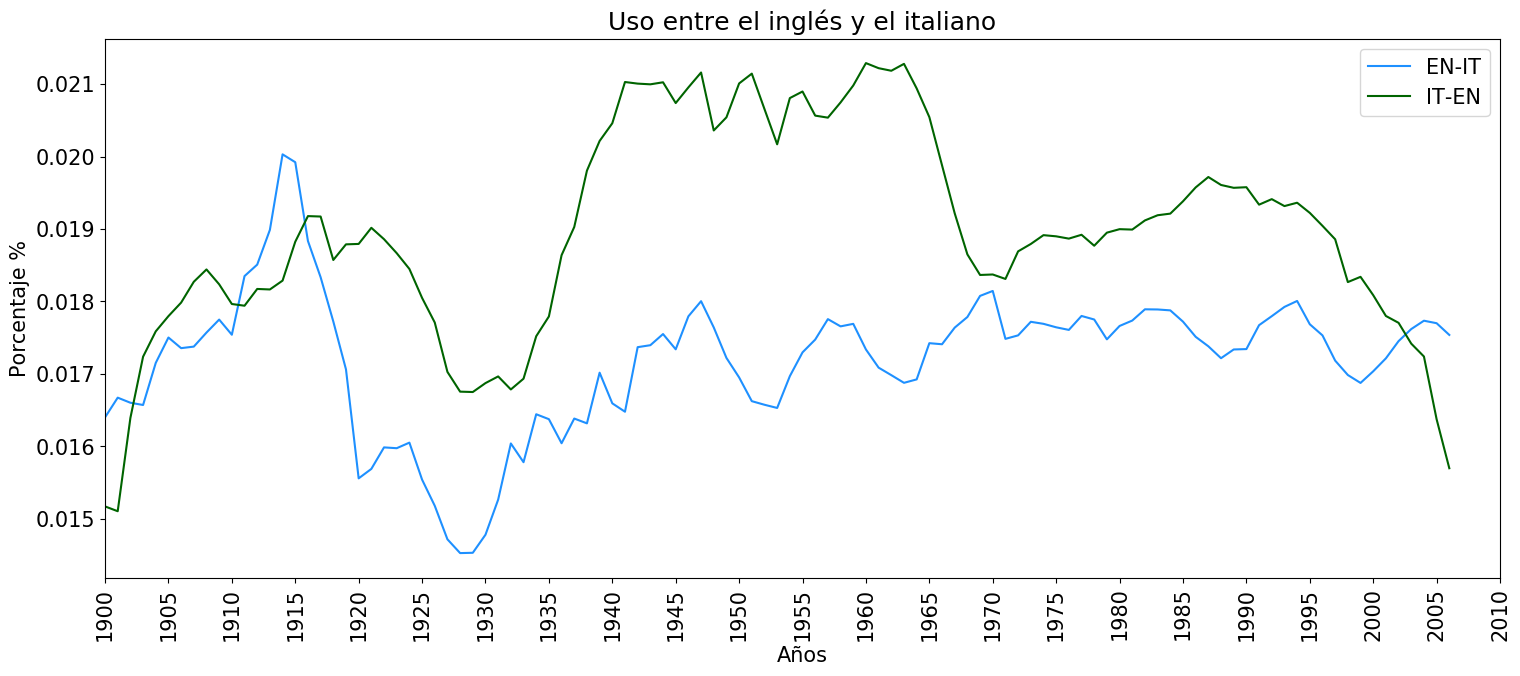
\includegraphics[scale=.38]{Cap_3/SF_3_S2_EN.png}
	\label{SF_EI}
	\caption{}
\end{figure}

Al retomar los resultados entre estos idiomas para los préstamos nuevos, las palabras del italiano al inglés no se lograron conectar a un hecho histórico que involucre a los dos idiomas, en los préstamos acumulados, el uso del italiano en el inglés predomina en un periodo más largo de tiempo (entre 1915 y el 2000) donde las palabras que constantemente aparecen son términos que provienen del griego y latín como test, inter, pure, format, regime, entre otras;  por lo que la influencia que tiene el italiano en el inglés se deben más a las raíces del italiano que también tiene el inglés.  

En el uso del inglés en el italiano,  hay dos periodos donde fue superior, el primero entre 1910 y 1915, donde el contenido predominante y que más se repite son verbos como be o do ( y sus diferentes conjugaciones),  el segundo periodo se da entre el 2000 y el 2005, donde la influencia del inglés supera a la del italiano, al igual que en los casos anteriores donde estuvo involucrado el inglés, predominan las palabras de los temas que abarcan a la globalización. 


\newpage
\subsection{Inglés y Español}

\begin{figure}[h!]
	\centering
	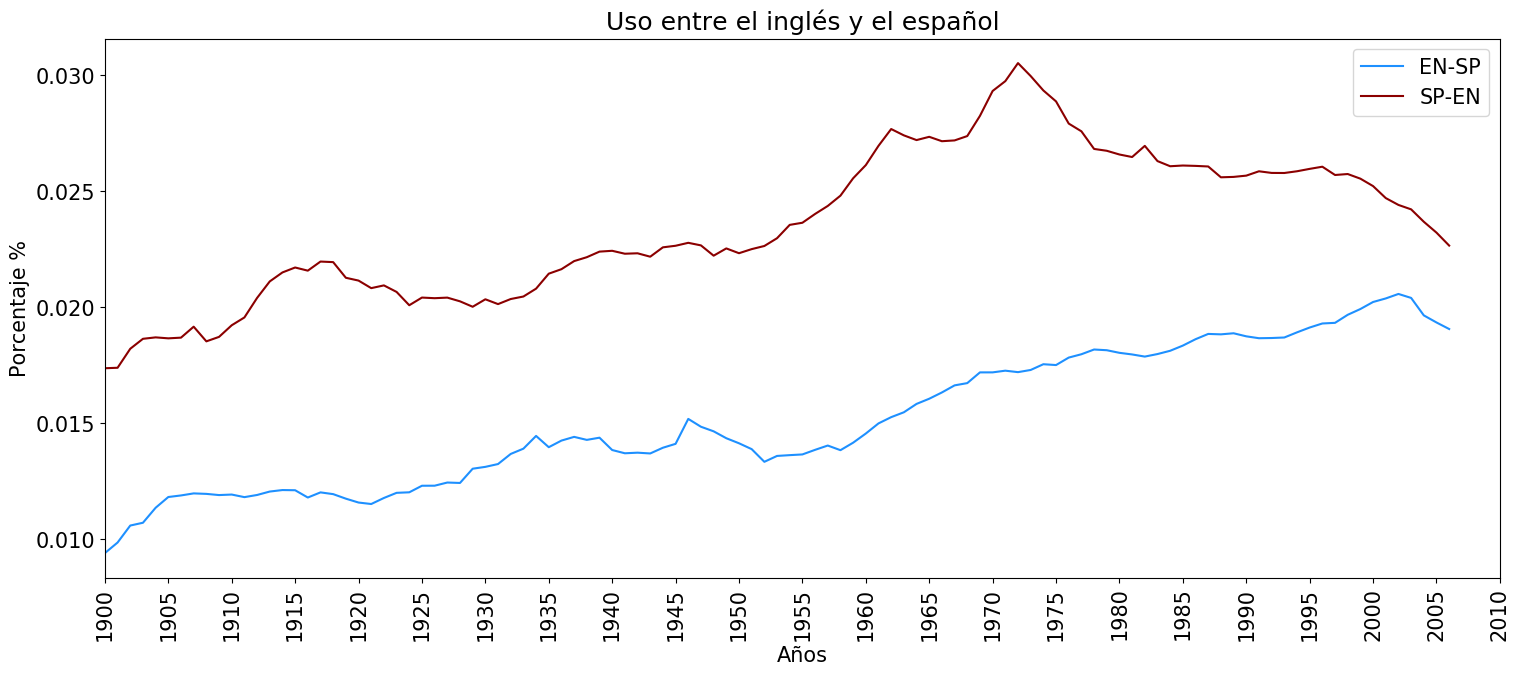
\includegraphics[scale=.38]{Cap_3/SF_4_S2_EN.png}
	\label{SF_ES}
	\caption{}
\end{figure}

El uso del inglés en el español es en todo momento menor,a diferencia de los resultados anteriores donde en algún periodo domina el uso del inglés.  En los más de cien años que se empleó el método el inglés creció desde un 0.01$\%$ hasta un casi 0.02$\%$, es decir casi 0.001$\%$ por cada década, siendo al momento el único caso donde el crecimiento es (casi) constante y no presenta un comportamiento repentino como el inglés en el francés o en el alemán a partir de 1990. No es viable decir que el crecimiento década a década continuará ocurriendo, ya que como se ha visto la espontaneidad de un evento modifica la forma en la que los idiomas interactúan entre sí, y el predecir la fecha de un suceso y el cómo afectará a los idiomas es imposible.  

Parte de las palabras que dan el incremento del uso del inglés en el español, se encuentran los verbos comunes del inglés be, do, have, estados y ciudades de Estados Unidos  como California, Texas, York, Chicago, y los términos relacionados al desarrollo global de los últimos años internet, mail, company.  Son importantes los nombres de ciudades y estados que aparecen, particularmente California y Texas, dos estados que concentran gran parte del producto interno de los Estados Unidos y la sede de industrias que más han crecido en los últimos años como la tecnológica,  la de energías, la aeroespacial y  la del entretenimiento; también son importante estos estados por la su historia con ambos idiomas, desde que el territorio de ambos pertenecía  a México,  su posterior anexión a los Estados Unidos por las guerras  de intervención,  y actualmente por ser lugares donde al radican inmigrantes ocasionando que la porción de la población de origen hispano aumente cada año. .

A pesar de los factores mencionados como responsables del crecimiento del inglés en el español,  el uso del español en el inglés es mayor , una razón de ello la da [XXXX] donde explica la tendencia del español antiguo a nacionalizar los términos que eran ajenos a él y que tuvo repercusiones aún en el siglo XX; es decir, si los conceptos que llegaban a España adoptaron una nueva escritura acorde al castellano,  reduciendo los préstamos (iguales en escritura)  y su uso en el español, al adoptarlos como propios. Si el nacionalizar palabras al español afectó a los demás idiomas, entonces el uso de cualquier idioma en el español es menor al uso del español en ese idioma, lo cual se comprobará en los siguientes resultados.



\subsection{Francés y Alemán}

\begin{figure}[h!]
	\centering
	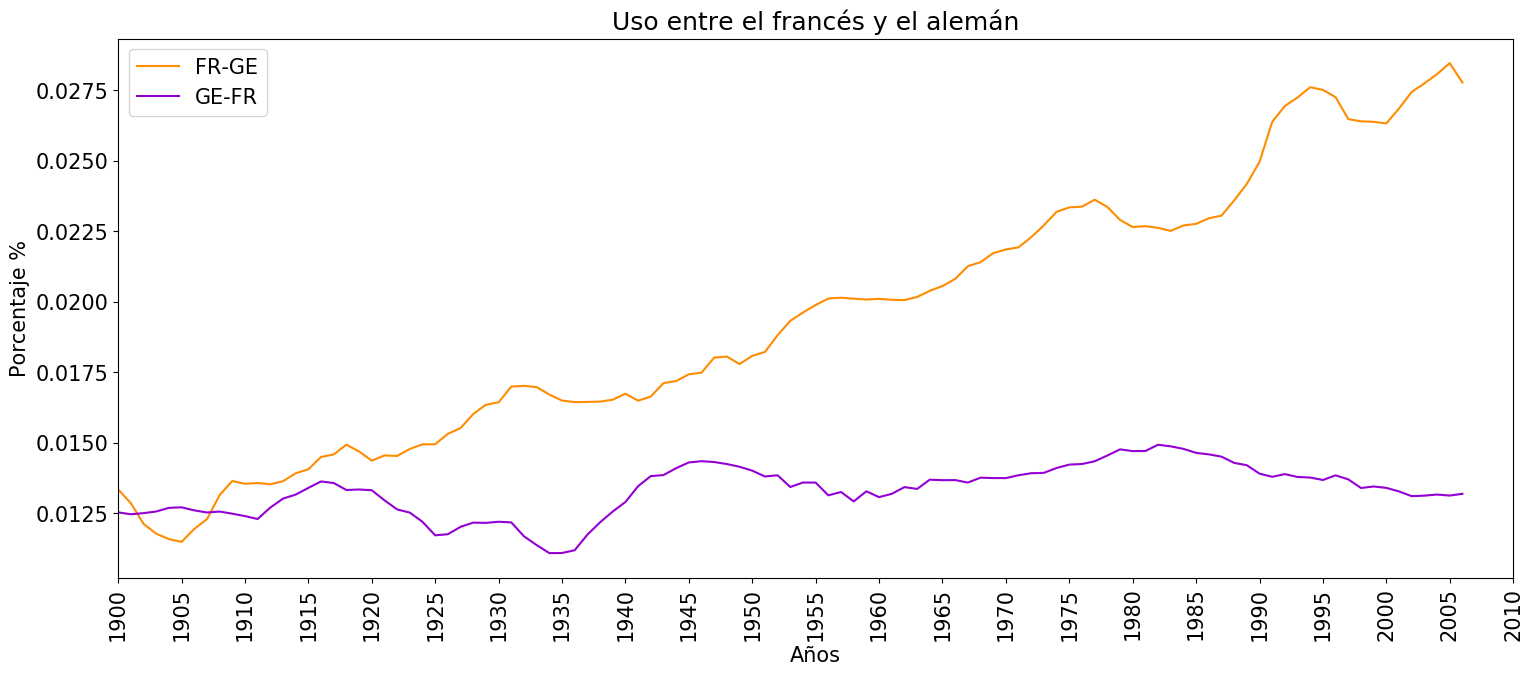
\includegraphics[scale=.38]{Cap_3/SF_2_S2_FR.png}
	\label{SF_FG}
	\caption{}
\end{figure}

Los préstamos provenientes del francés que recibe el alemán predominan en uso sobre los del alemán hacia el francés, aumentando la diferencia en cada año que transcurre.  En los años donde el alemán predominó sobre el francés (1900-1905) se encuentran términos médicos como anatomie, chirurgie, physiologie, psychologie y tuberculose, exponiendo cuán importante resultaron las investigaciones medicinas hechas en la Europa central.  En las listas posteriores comienzan a desaparecer los términos médicos, hasta que emerge la palabra Freud donde en cada año que aparece, también lo hace psychologie.  A pesar de que el crecimiento del alemán en el francés no es tan grande como en el sentido opuesto,  el año de 1935  hay otra erupción de palabras que repiten en cada año, estas ya se han mencionado en los préstamos nuevos y son referentes a la segunda guerra mundial. 

Los campos a los que se asocian los préstamos del francés al alemán son más diversos, desde la religión e ideologías políticas  en la primera mitad de siglo, hasta conceptos de la industria en la segunda mitad. Destaca que a pesar de los sucesos en los que se vieron involucrados países de habla francesa y alemana, el uso del francés ha sido creciente en el alemán  a pesar de la variedad de conceptos donde los préstamos son utilizados. 


\subsection{Francés e Italiano}

\begin{figure}[h!]
	\centering
	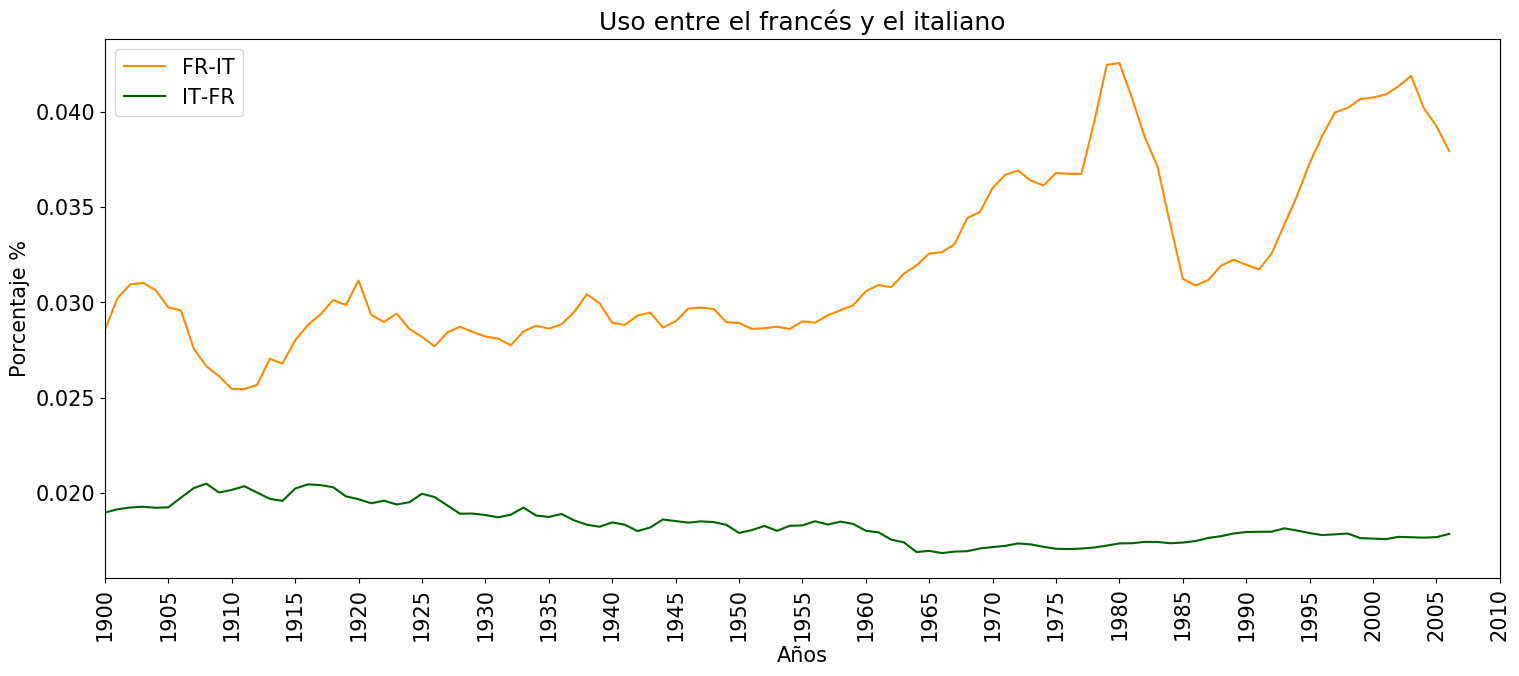
\includegraphics[scale=.38]{Cap_3/SF_3_S2_FR.png}
	\label{SF_FI}
	\caption{}
\end{figure}


El uso del francés en el italiano muestra tres periodos donde creció repentinamente, el primero entre 1915 y 1920, el segundo entre 1955 y 1980 y el tercero  entre 1990 y 2005.  La diversidad de tema donde pueden usarse los préstamos del francés en el italiano dificulta establecer una razón que explique los incrementos, el tener una variedad de temas caracterizó al francés como un idioma amplio  en contenido,  ya que la misma propiedad se encontró para los préstamos del francés al alemán.  Un factor general para los incrementos en el tercer periodo se debe a la globalización,  por la erupción de palabras  técnicas afines al área (economie, industrie,  capitale) aunque estas se encuentren en otros idiomas, son constantemente repetidas en las listas desde 1991 hasta 2007. 

Al analizar los préstamos en sentido opuesto, es decir los que van del italiano al francés,  la gráfica no presenta modificaciones drásticas en su uso,  siempre manteniéndose alrededor del 0.02$\%$. El contenido muestra vocablos que relacionan a los países de Italia y Francia, como lo es la palabra vigne  (traducción de viñedo) que vincula la industria vitivinícola donde ambos países tienen presencia

\newpage
\subsection{Francés y Español}


\begin{figure}[h!]
	\centering
	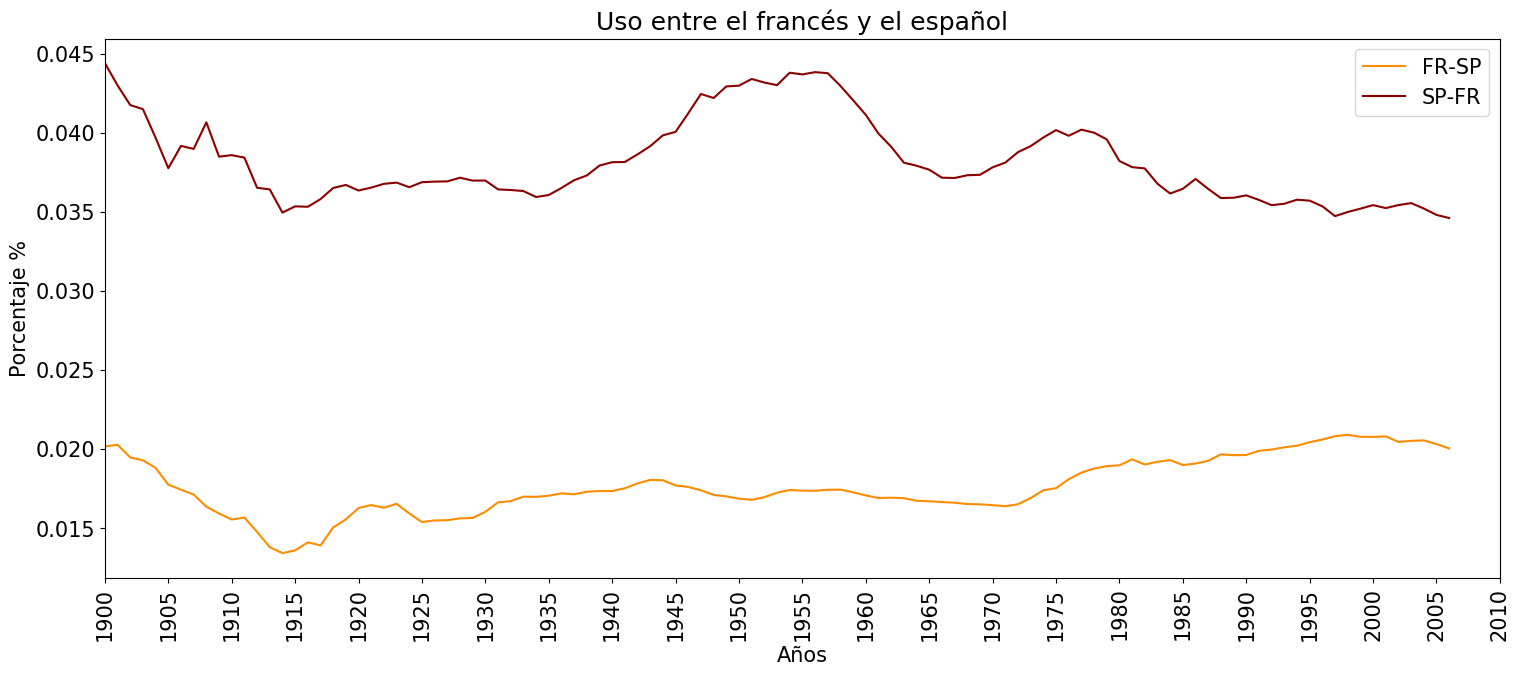
\includegraphics[scale=.38]{Cap_3/SF_4_S2_FR.png}
	\label{SF_FS}
	\caption{}
\end{figure}



Entre ambos idiomas, el español ha sido más utilizado en el francés durante el siglo pasado,  teniendo en cada década una diferencia del 0.02$\%$ , aunque hay una diferencia entre los usos, la lista de préstamos en ambos idiomas receptores muestran palabras que difícilmente podrían ser catalogadas como préstamos, es decir ya son palabras que por su familiaridad con el idioma receptor ya es común pensarlas como si siempre hubiesen formado parte del idioma.   

Una razón de la familiaridad entre el francés y el español se da por  provenir ambas de la familia de las lenguas romances, donde la mayoría de las palabras tienen el mismo origen etimológico dificultando el responder quien ha tenido una mayor influencia. Por la antigüedad de los mismos idiomas y su relación común en el greco latin, sí existió un periodo donde la adopción de nuevas palabras modificó el uso de los idiomas, tal período puede ser igualmente antiguo y las palabras nuevas se han adaptado al receptor de tal forma que siguen la tendencia del uso del mismo, es decir el uso de  la palabra “París” en el español se comporta como el uso de todas las palabras en español sin importar su distinción si provienen de un idioma determinado o son de origen español.  Esta premisa se verificará en las últimas secciones del escrito y se espera se cumpla para las lenguas romances del trabajo ( francés italiano y español)



\newpage
\subsection{Alemán e Italiano}

\begin{figure}[h!]
	\centering
	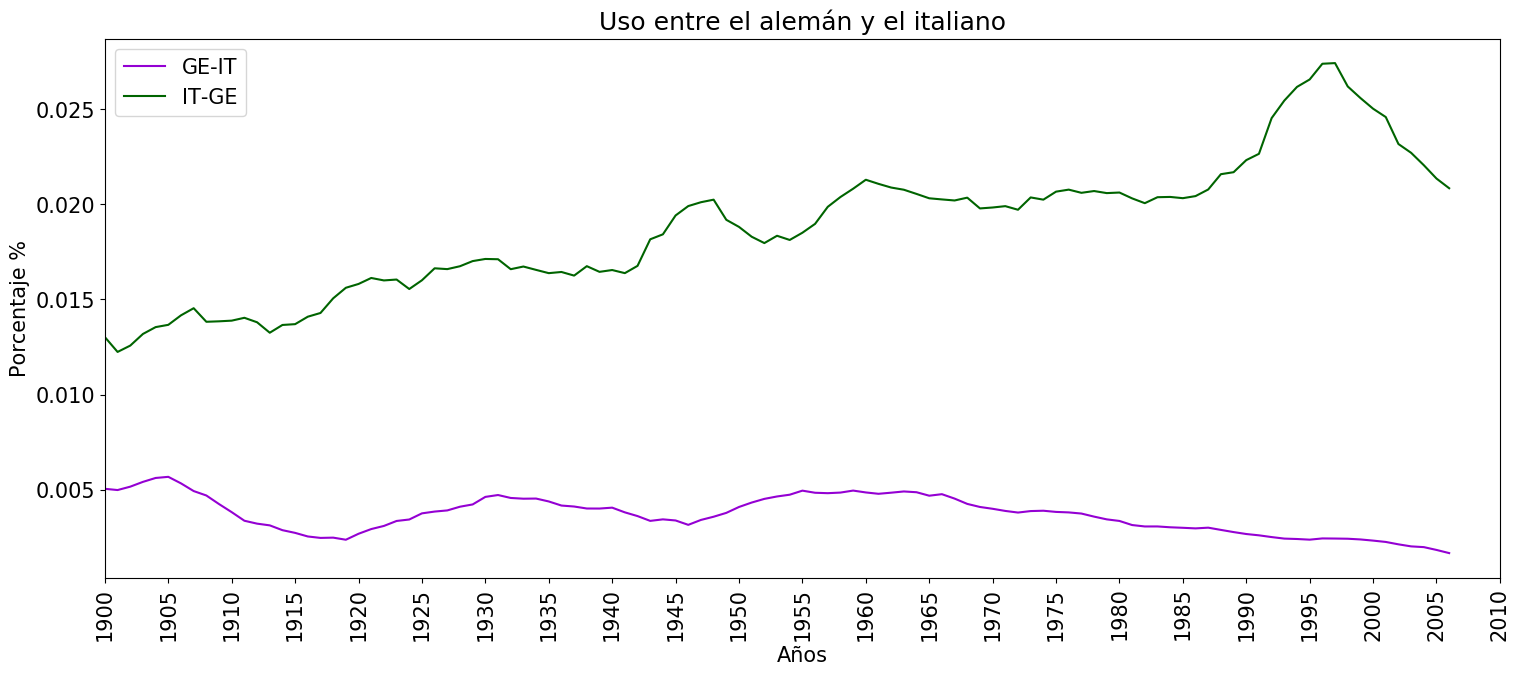
\includegraphics[scale=.38]{Cap_3/SF_3_S2_GE.png}
	\label{SF_GI}
	\caption{}
\end{figure}

El uso del italiano en el alemán ha incrementado en el siglo XIX, por la historia entre las naciones con estos idiomas oficiales,  destaca nuevamente la presencia de la palabra Mussolini  continuamente desde 1935 hasta 1953, y alternando periodos de aparición de uno o dos años  con desapariciones por el mismo tiempo. En los mismos años donde aparece Mussolini se encuentran las palabras de regime, status, schema, liberale y Ribbentrop  (estas palabras ya se habían tratado en los préstamos nuevos) en diferentes posiciones de rango pero dentro de la misma lista; el tener este conjunto del mismo campo semántico, que dentro de los años de aparición haya sucedido la segunda guerra mundial y que el uso del italiano en el alemán haya aumentado y disminuido en casi las mismas fechas hace posible las conexiones entre estas variables, es decir la guerra propició a que las palabras relacionadas al conflicto alterarán el uso del italiano en el alemán.    El último incremento se dio antes del año 2000,  siendo una característica que el alemán ha presentado en los análisis anteriores, el inglés  y francés también crecieron antes del año dos mil en el alemán, por lo que debe de ser una tendencia general del idioma alemán el crecer en esta fecha. 

Los préstamos del alemán no muestran un cambio relevante en la forma en que son utilizados en el italiano,  pero si hay diferencias entre el contenido de las listas en las dos mitades de siglo,  destacan en la primera mitad ciudades alemanas como Berlín, Leipzig, y en la segunda los apellidos de personajes germanófonos mencionados en los préstamos nuevos.  La presencia de los apellidos, muestra la relevancia que lograron los personajes en sus respectivos campos,  al ser constantes en las listas. 


\newpage
\subsection{Alemán y Español}

\begin{figure}[h!]
	\centering
	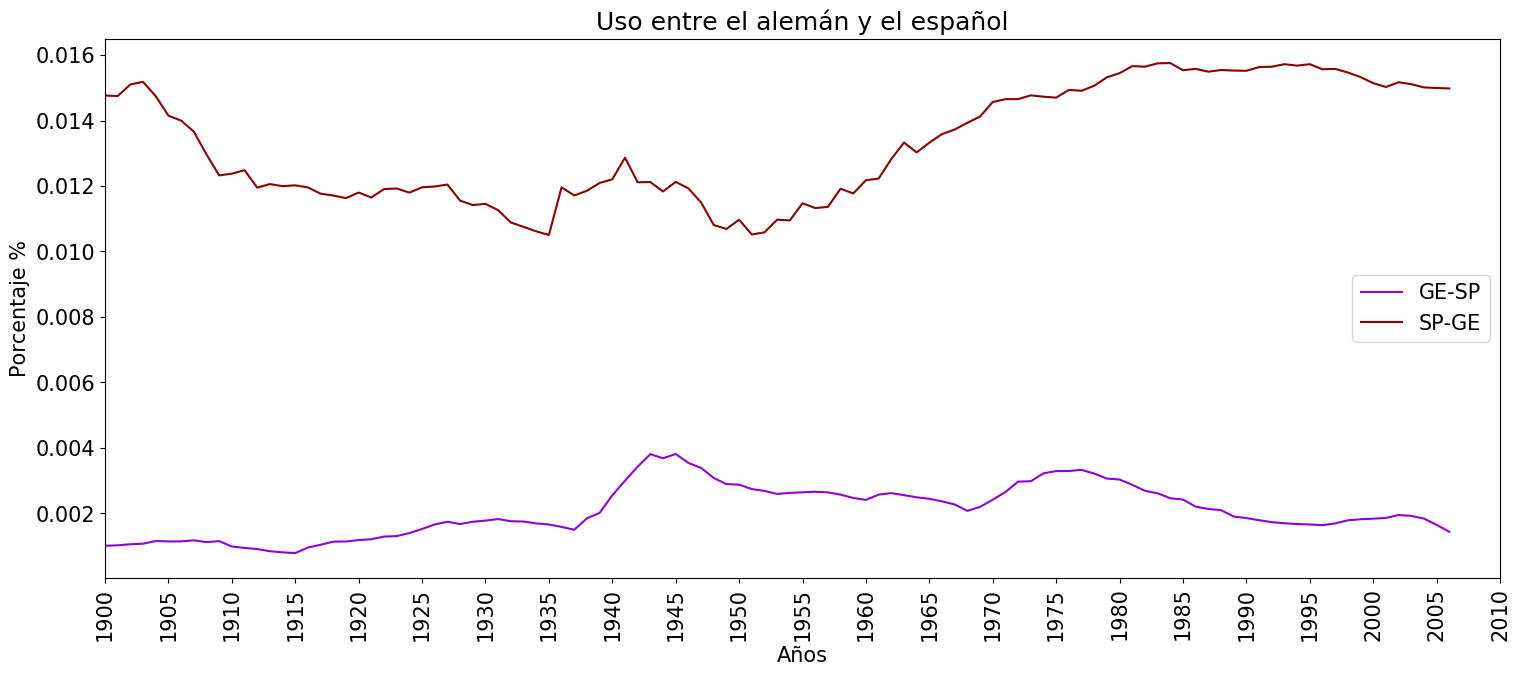
\includegraphics[scale=.38]{Cap_3/SF_4_S2_GE.png}
	\label{SF_GS}
	\caption{}
\end{figure}

Entre el uso de un idioma en el otro,  es escaso el utilizar palabras del alemán en el español, siendo el más pequeño  (entre el 0.002$\%$ y 0.004$\%$) entre todas las combinaciones hechas, su mayor ascenso comenzó en 1935 y su estabilidad se dio de 1945 a 1985,  épocas donde los pueblos germanófonos y sus hablantes  fueron citados por su papel en la historia y las consecuencias que originaron en diferentes ámbitos.  Dentro de las palabras que no se han mencionado, se encuentran metal y mineral,  donde estas fueron clasificadas como de origen alemán por ser el idioma donde tenían más relevancia al principio de las mediciones, aparecen en el español  por ser  la industria metalúrgica una de las actividades que caracterizaron a los países hispanos como productores, y su importancia en el alemán por ser la misma industria una de las bases de la revolución industrial alemana en el siglo XIX. 

El periodo donde los préstamos del español al alemán comenzaron a aumentar también comienza en 1935  manteniendo la misma tendencia hasta 1945,  coincidiendo con el pequeño apogeo del alemán en el español.  La lista de palabras no muestra coincidencias entre las palabras y el evento bélico de la época, sin embargo las palabras más repetidas a partir de ese año de crecimiento son  general, américa, capital, europa y washington, términos que bien pueden ser usados dentro del mismo contexto histórico de la postguerra. 



\newpage
\subsection{Italiano y Español}

\begin{figure}[h!]
	\centering
	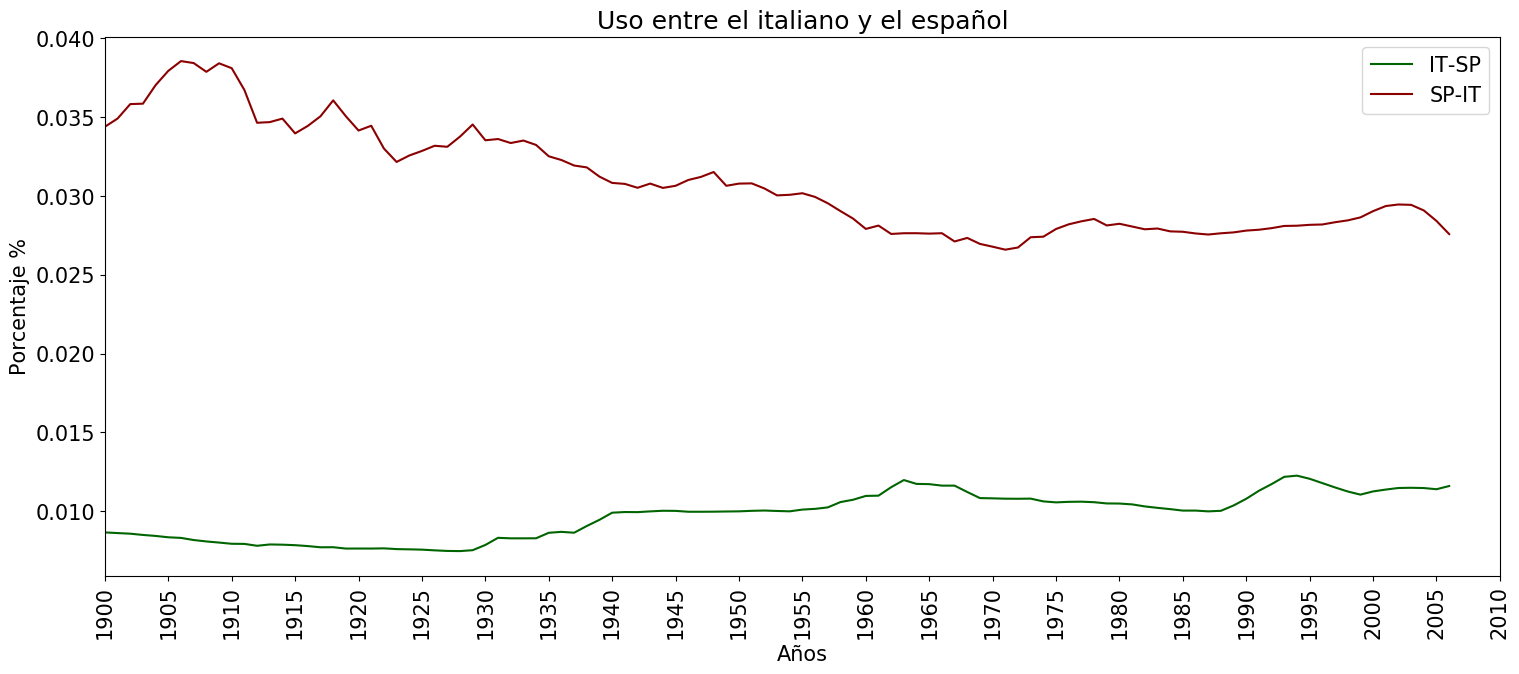
\includegraphics[scale=.38]{Cap_3/SF_4_S2_IT.png}
	\label{SF_IS}
	\caption{}
\end{figure}

El comportamiento entre estos idiomas es similar al calculado entre el francés y el español, donde el uso del español predomina.  Nuevamente se están tratando dos lenguas romances  que comparten muchas palabras de la misma rama etimológica y donde una palabra puede ser común en el receptor aunque se haya clasificado como nueva o de un determinado origen.     

De estas palabras catalogadas como de origen español,  a pesar de ser ampliamente utilizadas en el italiano, su uso ha decaído aunque esta puede ser una tendencia del italiano por sí mismo ya que el comportamiento de los demás idiomas en el italiano ha decaído en los últimos veinticinco años (desde 1985). 

Por parte de los préstamos del italiano usados en el español,  su uso aunque mínimo ha incrementado desde 1930,  parte de este incremento pueden ser por el auge en publicaciones de américa latina,  al encontrar palabras como realismo, latina, o narrativa, además de los  términos asociados a ideologías políticas que igualmente ya se comentaron en los préstamos nuevos del italiano al español, y que perduraron en el siglo pasado.



\newpage
\section{La cantidad de préstamos acumulados y el uso en conjunto}

En los comentarios pasados  se ha mencionado las palabras que forman parte de las listas de los préstamos acumulados, y como algunas de ellas han logrado modificar el uso de un idioma en otro. También se ha especificado que el uso de un idioma en otro se obtiene por la frecuencia de las palabras que conforman la lista, más no por la cantidad de ellas. Para aclarar esta hipótesis,  se realizó la tabla [XXXX]]] mostrando el promedio de palabras con origen A que se encuentran en las listas de B. 

\hfill\break

\begin{table}[h!]
	\centering
	\begin{tabular}{lcccccc}
		\multicolumn{7}{c}{R E C E P T O R}                                                                                                                                             \\
		\multirow{6}{*}{\begin{tabular}[c]{@{}l@{}}O\\ R\\ \,I\\ G\\ E\\ N\end{tabular}} &             & \textbf{EN} & \textbf{FR} & \textbf{GE} & \textbf{IT} & \textbf{SP} \\
		& \textbf{EN} & -           & 324.43      & 164.33      & 77.5        & 73.61       \\
		& \textbf{FR} & 297.36      & -           & 94.06       & 118.55      & 66.31       \\
		& \textbf{GE} & 63.87       & 48.06       & -           & 34.92       & 16.61       \\
		& \textbf{IT} & 77.82       & 100.62      & 47.9        & -           & 219.45      \\
		& \textbf{SP} & 118.43      & 84.22       & 29.85       & 311.97      & -          
	\end{tabular}
	\caption{}
	\label{T_PA}
\end{table}




De la tabla se aprecian dos relaciones similares entre la cantidad de palabras, la primera entre el inglés y el francés si se escoge uno de estos dos idiomas como el idioma origen, entonces el otro funge como el receptor donde las palabras del origen son mayoritarias; la misma característica ocurre con el italiano y el español.  Las relación entre el español y el italiano es esperada, al provenir ambas de la familia de las lenguas romances, la composición etimológica de sus vocablos es semejante,  resultando en una mejor adaptación en el idioma receptor. 

Ahora para decir con seguridad cuál idioma es más influyente en otro,  se realizarón dos gráficas de influencia en conjunto, para ello se requirió de un idioma origen A y de los diferentes idiomas receptors B, C, D y E.  La primera gráfica consiste en ver  el uso de los préstamos de A que llegan a los diferentes receptores pero visualizados todos en una misma gráfica,  es decir estará el uso de A en B, el de A en C y así sucesivamente,  con ello se determina y por cuáles periodos  A es más influyente.   La segunda gráfica de conjunto, se intercambian los idiomas receptores por orígenes, y se grafican el uso de los demás idiomas en el idioma receptor A, para  sostener el argumento de cual idioma ha influenciado más al idioma A.       

Lo interesante de estas gráficas es que  muestra todos los comportamientos de un idioma en los demás, y de los demás en el idioma,  ya no es solo ver los préstamos de A en B y los de B en A. La tabla anterior es útil para ver que en pocos casos se cumple que el idioma que más palabras tiene es el más utilizado. 

\newpage
\subsection{Inglés}


\begin{figure}[h!]
	
	\begin{subfigure}{}
		\centering
		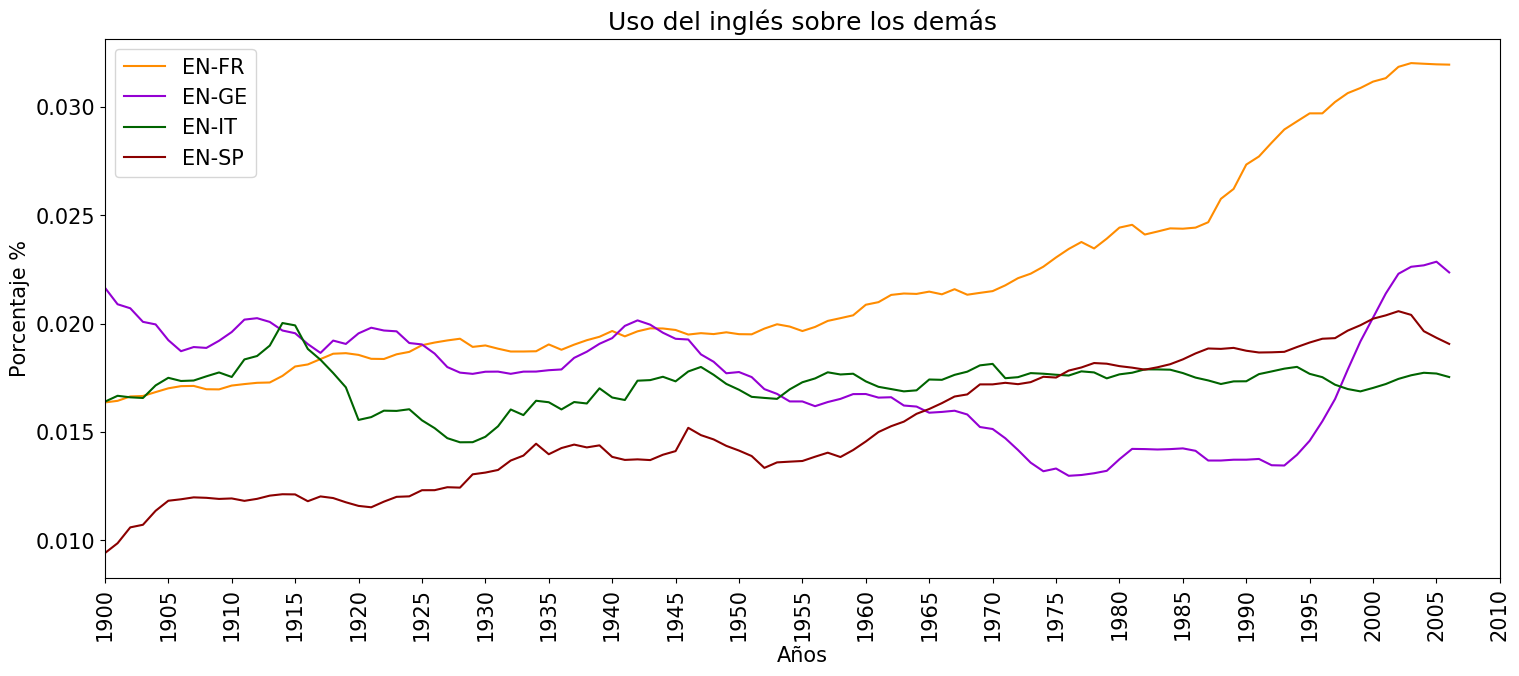
\includegraphics[scale=.38]{Cap_3/PF1_S2_EN.png}
		\caption{}
		\label{fig:ST_EN_a}
	\end{subfigure}
	
	\begin{subfigure}{}
		\centering
		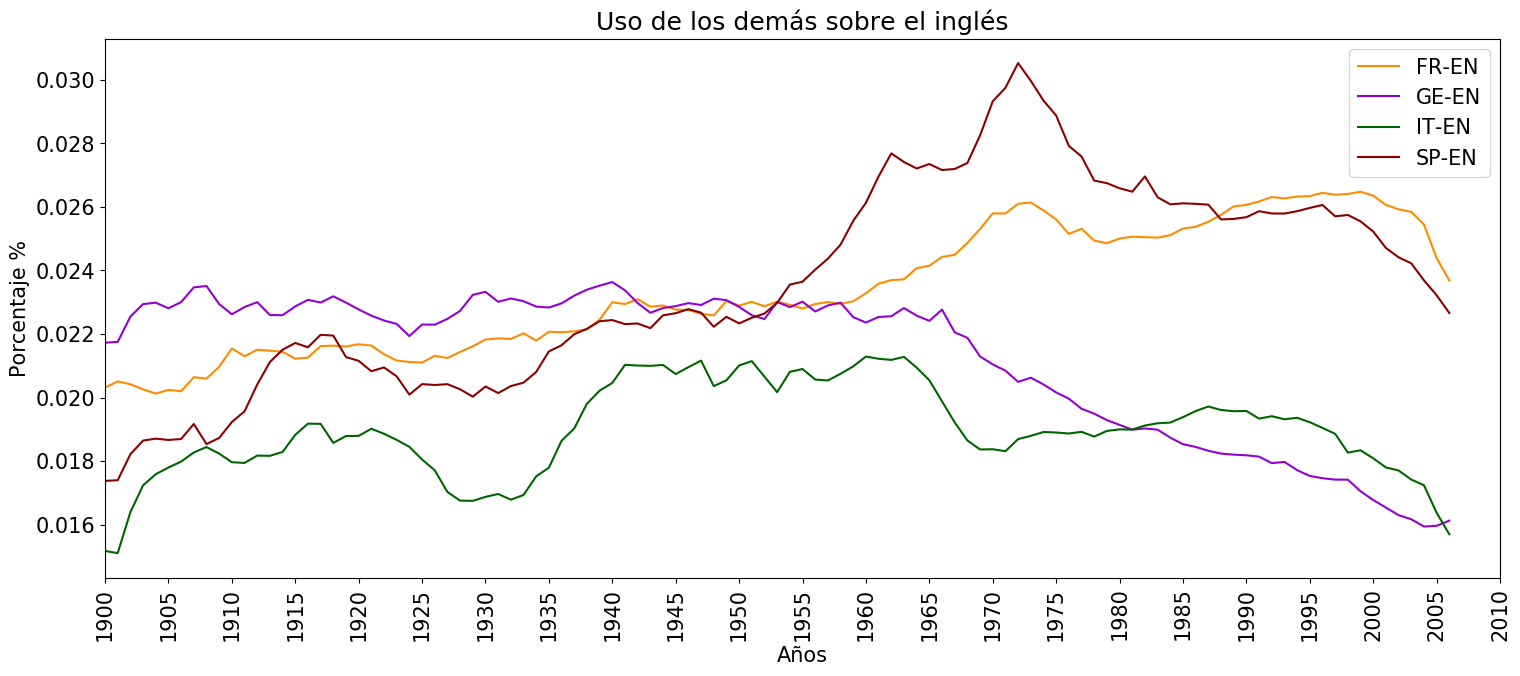
\includegraphics[scale=.38]{Cap_3/PF2_S2_EN.png}
		\caption{}
		\label{fig:ST_EN_b}
	\end{subfigure}
	
\end{figure}


Tomando al inglés como idioma origen, antes de 1945 su uso era similar entre el francés, el alemán y el italiano. Involucrando a la historia en la razón del crecimiento,  Alemania e Italia  fueron dos de los países perdedores de la segunda guerra mundial, por otra parte Estados Unidos (mayoritariamente), el Reino Unido y Francia se catalogaron como vencedores; siendo el periodo posguerra donde Estados Unidos se revalorizó como un país con poderío armamentista, con presencia en múltiples industrias, y con un modelo económico estable y que hasta el momento la mayoría de los países utiliza, incentivando el uso del inglés como idioma común entre países; el aspecto económico se refleja en en la gráfica del alemán, donde el incremento del inglés se da en años posteriores a 1990 donde en Alemania se termina el uso del otro modelo económico, con la disolución de la Unión Soviética, y donde comienza el dominio del mercado estadounidense con la cotidianidad de la tecnología y el internet. 

Aspectos como la proximidad geográfica entre Estados Unidos con Latinoamérica,  el aumento de las migraciones de personas entre ambos costados (siendo mayor el flujo hacia Estados Unidos),  las relaciones diplomáticas y de mercado surgen como posibilidades no solo del crecimiento del inglés en el español, sino también en el sentido opuesto, del español en el inglés, reflejado en el segundo gráfico, donde el español alcanza su punto más alto en 1970, de acuerdo a [XXXXXX] año donde se dio el mayor flujo de migrantes a Estados Unidos,  y a partir de donde empezó a crecer la comunidad hispana en el país. 


En el segundo gráfico,  el uso de los demás idiomas en el inglés se estabiliza entre los vales de  0.020$\%$ y 0.024$\%$  en los años de 1940 y 1955,  nuevamente, período que comprende el término de la segunda guerra mundial, el comienzo de la guerra fría y la división del mundo en dos bloques económicos,  salvo por el español que comenzó a ser el idioma más usado en el inglés a partir de 1950 (aspecto ya mencionado), mientras que los demás idiomas continúan con la misma relevancia  hasta principios de 1960.  De forma general el uso en el inglés decae en  1990 a partir de que el modelo económico de Estados Unidos es empleado por la mayoría de los países,  asimismo surge el desarrollo en las telecomunicaciones,  la globalización y nuevas herramientas como el internet, todas ellas donde el inglés es el medio natural para transmitir y compartir información. 


\newpage
\subsection{Francés}

\begin{figure}[h!]
	
	\begin{subfigure}{}
		\centering
		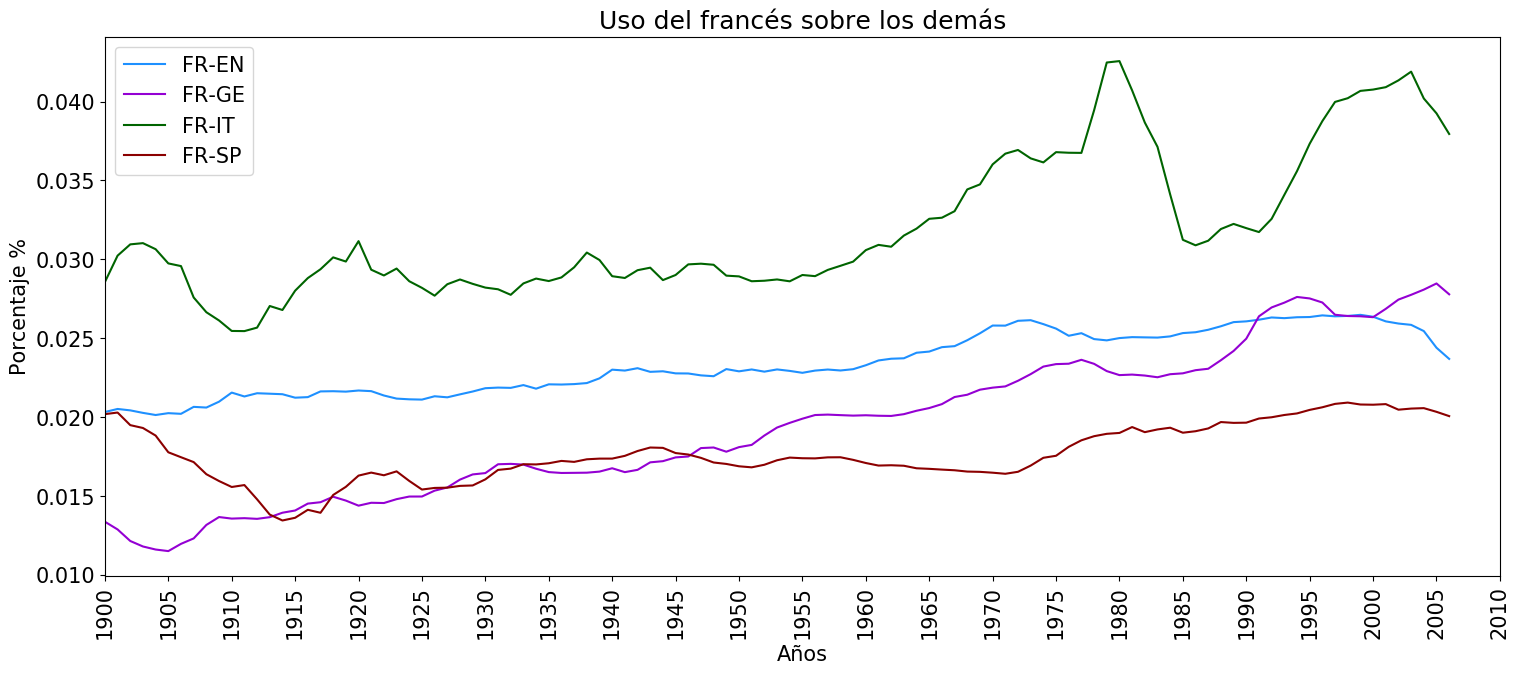
\includegraphics[scale=.38]{Cap_3/PF1_S2_FR.png}
		\caption{}
		\label{fig:ST_FR_a}
	\end{subfigure}
	
	\begin{subfigure}{}
		\centering
		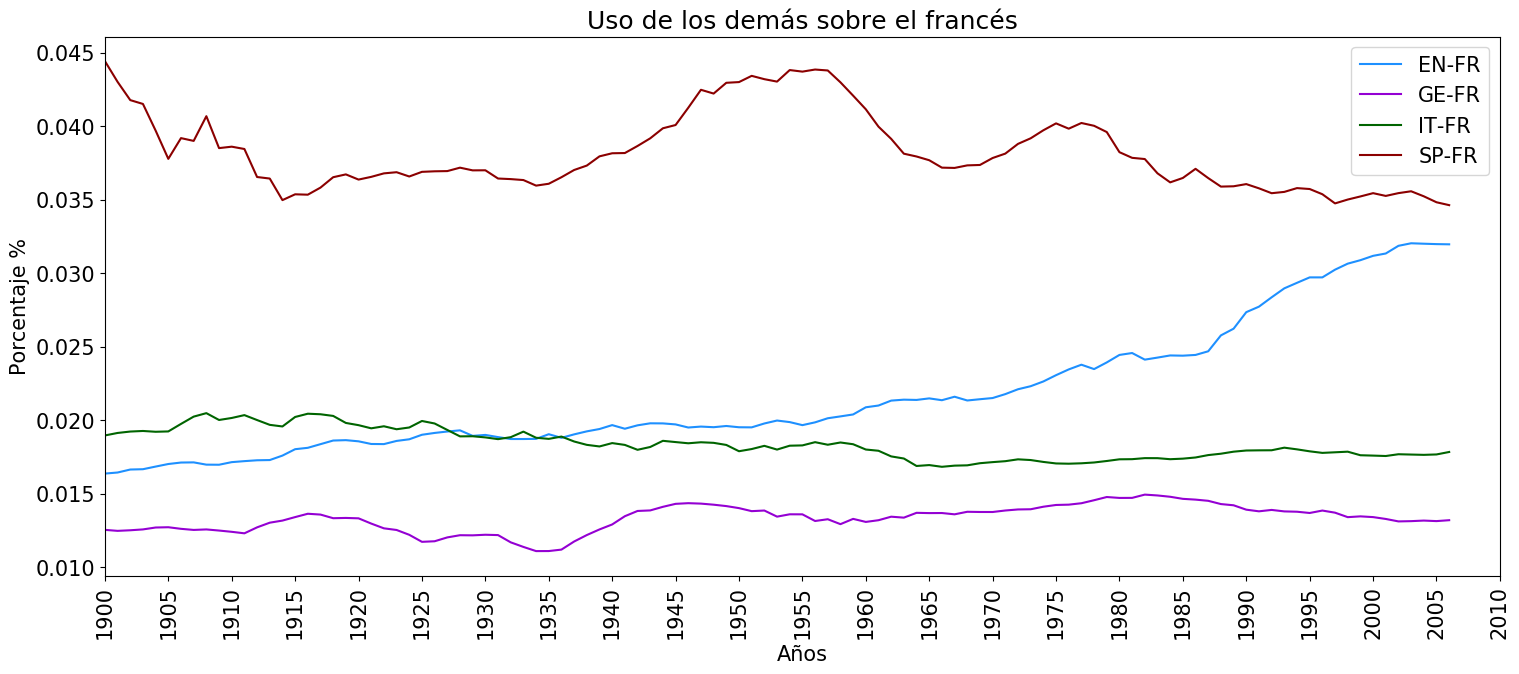
\includegraphics[scale=.38]{Cap_3/PF2_S2_FR.png}
		\caption{}
		\label{fig:ST_FR_b}
	\end{subfigure}
	
\end{figure}

A pesar de que el idioma que más préstamos toma del francés es el inglés,  el idioma que más utiliza el francés ha sido el italiano,  aspecto que se mantuvo durante todo el siglo del análisis.  Recapitulando lo comentado en los análisis de los préstamos,  el peso que tuvo la segunda guerra fue un detonante para que el uso entre los idiomas cambiase durante y posterior al conflicto,  en el caso del alemán y del inglés,  el empleo del francés en ellos aumentó tras finalizar el conflicto.  A pesar de que el español y el francés provienen de la familia de las lenguas romances,  el uso del francés en el español se ha mantenido sin mayores alteraciones.

El caso de cómo son utilizados los demás idiomas en el francés,  hay un dominio de las palabras con origen español, seguido por las de origen inglés; aunque el español ha sido el más empleado en el francés,  el inglés a partir de 1940 comienza a ser más frecuentado,  recortando en cado año la diferencia con el español,  siendo en la última parte del estudio  menor al 0.05$\%$, incluso si la base de datos abarcara más años posteriores al 2009, es probable que el uso el inglés pase al español. 


\newpage
\subsection{Alemán}

\begin{figure}[h!]
	
	\begin{subfigure}{}
		\centering
		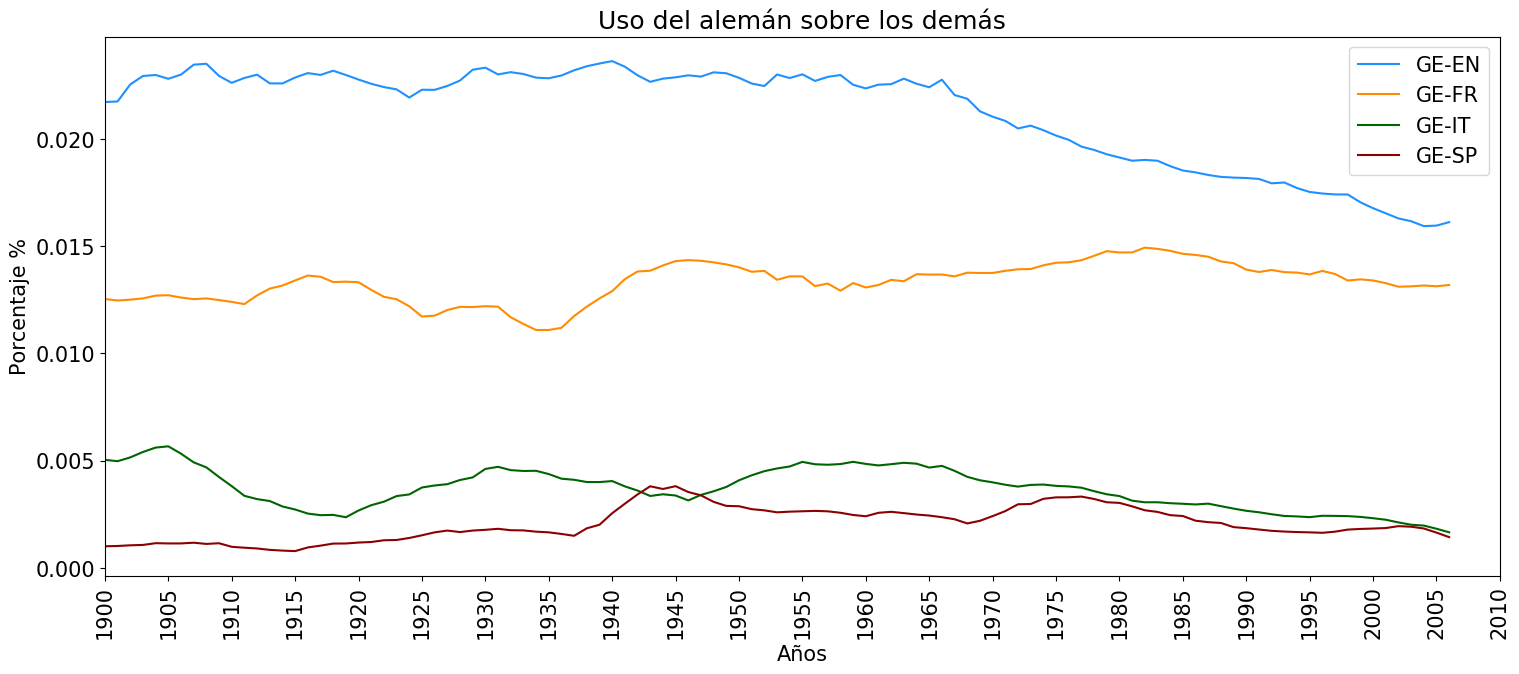
\includegraphics[scale=.38]{Cap_3/PF1_S2_GE.png}
		\caption{}
		\label{fig:ST_GE_a}
	\end{subfigure}
	
	\begin{subfigure}{}
		\centering
		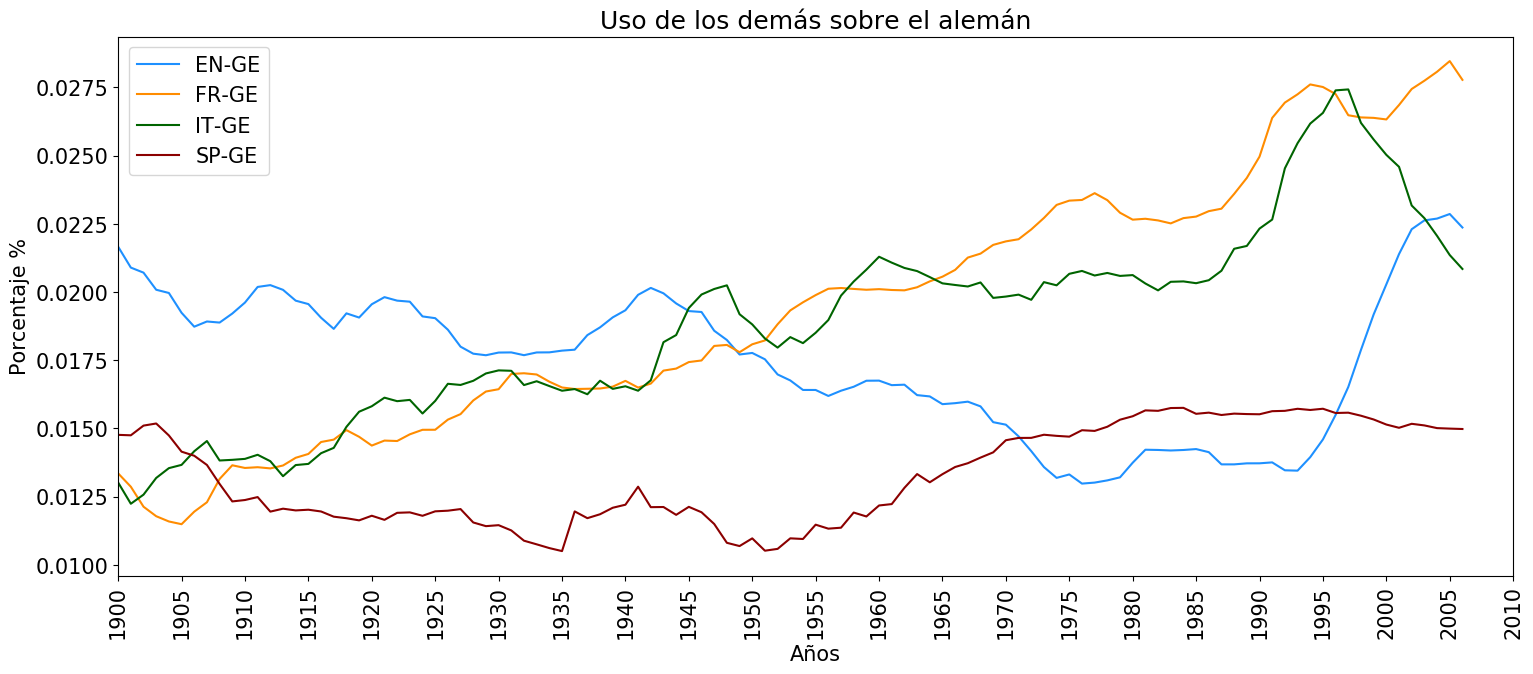
\includegraphics[scale=.38]{Cap_3/PF2_S2_GE.png}
		\caption{}
		\label{fig:ST_GE_b}
	\end{subfigure}
	
\end{figure}

De acuerdo a la tabla [XXX],  el inglés, el francés, el italiano y el español, son en ese orden idiomas que más préstamos tienen provenientes del alemán, a pesar de que el alemán sea en cada uno el idioma del que menos se componen.  El orden de los idiomas que más emplean el alemán es el mismo que los idiomas que más se componen del alemán, siendo el único caso donde la mayor cantidad es también el mayor uso. Una razón de esta característica es que tanto el alemán como el inglés provienen de la misma familia lingüística, la germánica,  siendo más comunes las palabras entre ellos  que con las lenguas romances.

El sentido de cómo se utilizan los demás idiomas en el alemán, no presenta la característica anterior,   donde se ha alternado entre el inglés, el francés y el italiano el idioma que es más utilizado en el alemán.  El inglés fue el más empleado en la primera mitad del siglo, mientras que posterior a la guerra que ha sido el común detonante para que se altere el uso de un idioma en otro,  francés e italiano rolaron el papel del idioma más común en el alemán. 


\newpage
\subsection{Italiano}

\begin{figure}[h!]
	
	\begin{subfigure}{}
		\centering
		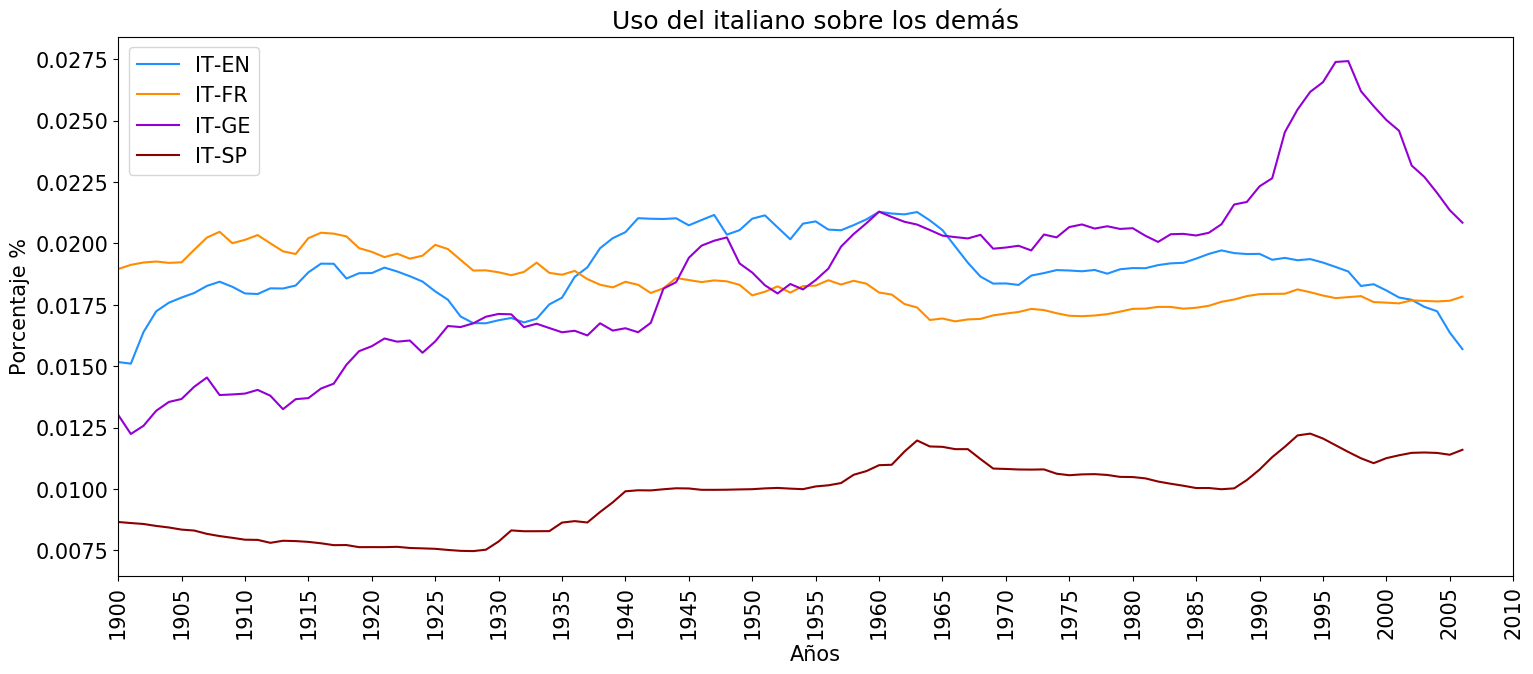
\includegraphics[scale=.38]{Cap_3/PF1_S2_IT.png}
		\caption{}
		\label{fig:ST_IT_a}
	\end{subfigure}
	
	\begin{subfigure}{}
		\centering
		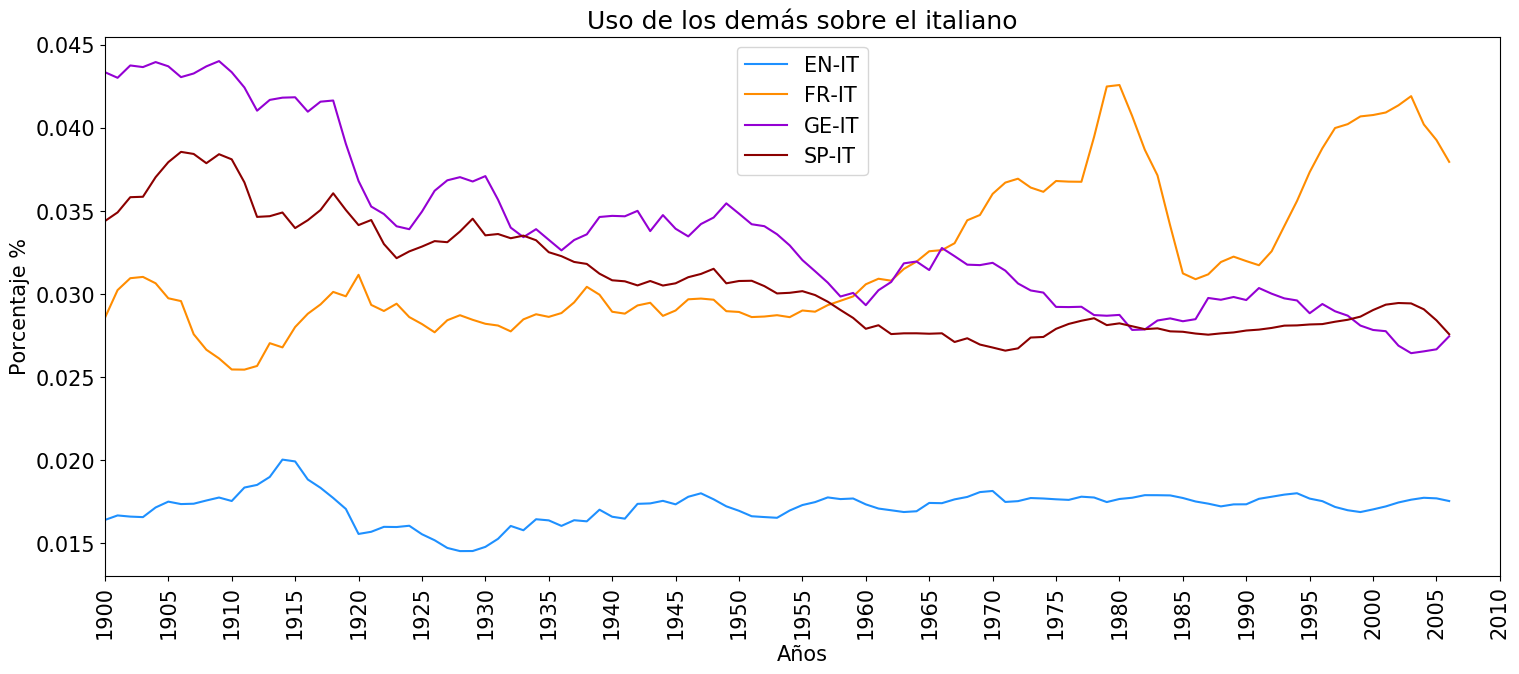
\includegraphics[scale=.38]{Cap_3/PF2_S2_IT.png}
		\caption{}
		\label{fig:ST_IT_b}
	\end{subfigure}
	
\end{figure}

Los idiomas en los que el italiano ha tenido una mayor influencia han sido el inglés, el francés y el alemán pese a que el español es el idioma que más préstamos contiene del  italiano,  circunstancias como la cercanía geográfica entre los países de habla alemán con Italia alude al  mayor uso del italiano en este idioma a partir de  la segunda mitad del siglo,  respecto al inglés,  la intervención de personajes  italianos en la historia y el hecho de que el inglés se compone de palabras de origen grecolatino,  permite que el italiano sea una lengua fuerte en el inglés;  las afirmaciones anteriores se han respaldado en que las palabras de contenido han sido previamente relacionadas  a sucesos donde han intervenido estos países.


La forma de actuar de los demás idiomas en el italiano no es recíproca a la forma en que el italiano interviene en ellos.  El caso del inglés es particular, porque a pesar del impacto que ha manifestado el inglés en los demás idiomas  en los últimos cincuenta años por la globalización,  en el italiano ha sido el único idioma donde no ha sido dominante en algún punto, o donde no ha crecido más que los demás.  El alemán ha sido más importante al comienzo del siglo y decae tras finalizar la segunda guerra mundial, para imponerse el francés como el idioma que más es utilizado en el italiano. 


\newpage
\subsection{Español}


\begin{figure}[h!]
	
	\begin{subfigure}{}
		\centering
		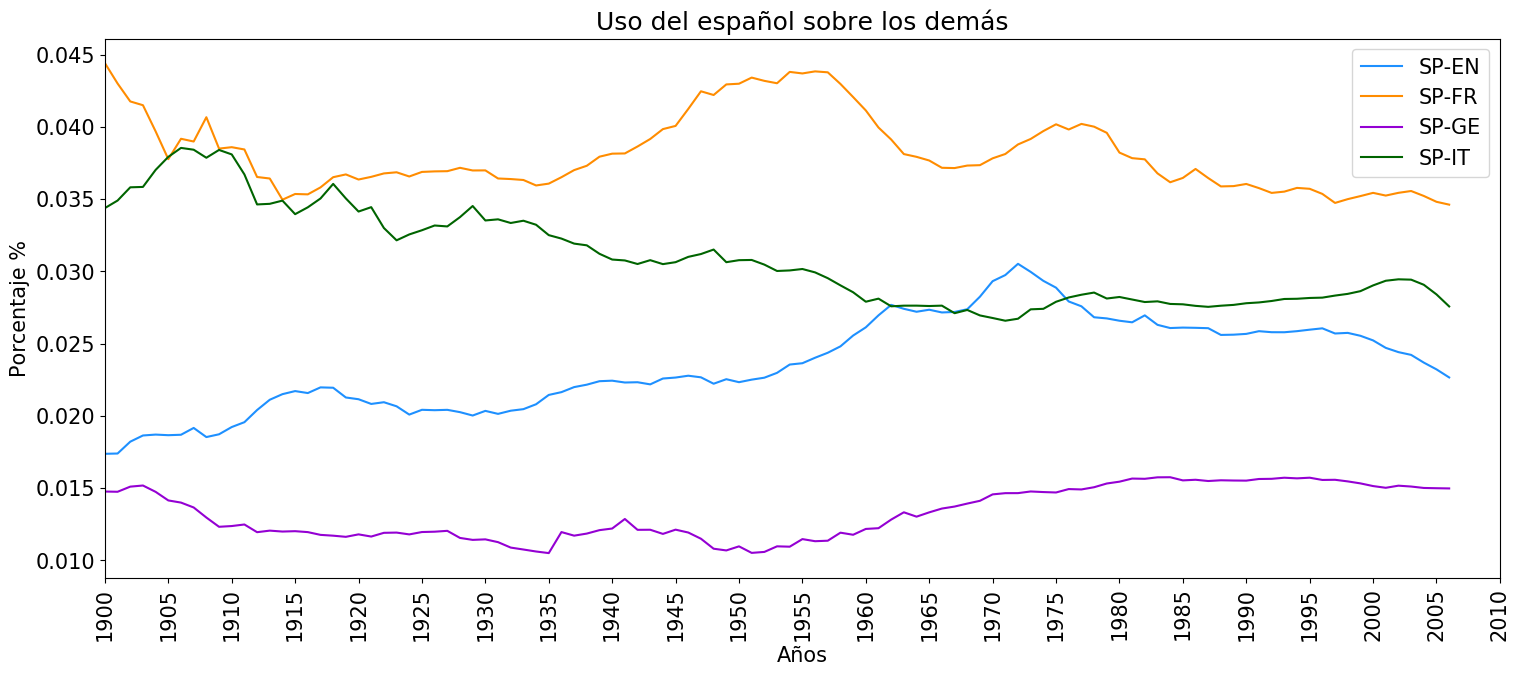
\includegraphics[scale=.38]{Cap_3/PF1_S2_SP.png}
		\caption{}
		\label{fig:ST_SP_a}
	\end{subfigure}
	
	\begin{subfigure}{}
		\centering
		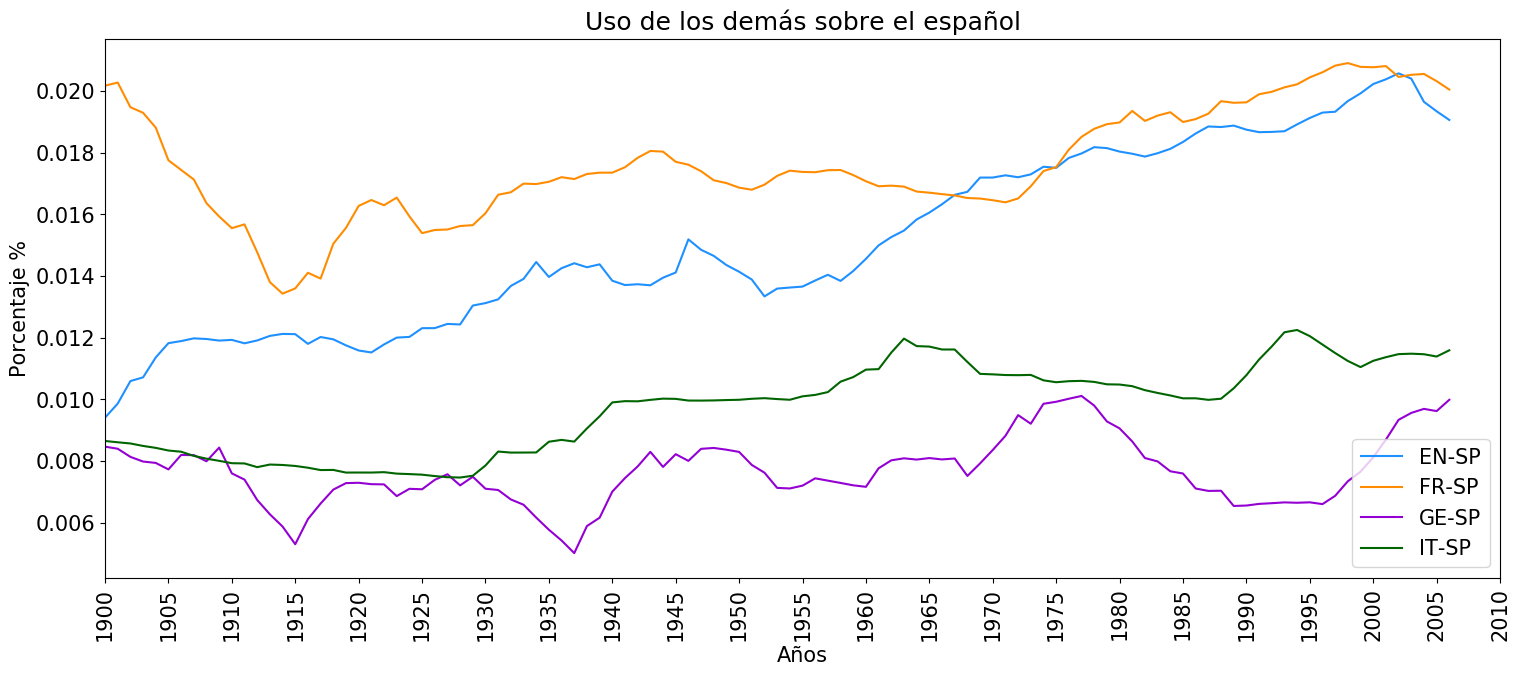
\includegraphics[scale=.38]{Cap_3/PF2_S2_SP.png}
		\caption{}
		\label{fig:ST_SP_b}
	\end{subfigure}
	
\end{figure}


Entre los gráficos de uso entre un determinado idioma y el español, se observó que el español ha sido más influyente en los demás que los demás en él,  siendo el francés el idioma donde el español es más utilizado, a pesar de que la cantidad de préstamos que llegan al italiano es mayor.   Ya se han mencionado factores que condicionan la forma de las gráficas, siendo la más evidente, el provenir de la misma familia lingüística al ser el español más utilizado en el francés y el italiano. 

Entre la forma en la que se usan los préstamos de los demás idiomas en el español,  en los últimos cincuenta años, la mayor influencia se ve compartida entre las palabras que vienen del francés y  del inglés;  la familia de las lenguas romances y sus similitudes hacen posible que el francés tome relevancia, mientras que la globalización y el crecimiento económico de países de habla inglesa hace relevante al inglés en el español.   Por otro lado,  el italiano y el alemán  no presentan el mismo crecimiento que el francés y el inglés,  por parte del italiano se ha comentado que al ser lengua romance al igual que el español,  el periodo donde los préstamos modificaban el uso del idioma receptor pudiese ser tan antiguo como el surgimiento de los idiomas,  por ello comparten gran cantidad de palabras pero estas no alteran el comportamiento del receptor; mientras que en el caso del alemán la poca relación con el español y el no haber existido un evento que los involucren,  hace que estos idiomas no se hayan mezclado como los demás,  por ejemplo alrededor de 1915 y 1935,  el alemán en el español es casi nulo, a pesar de que en esas fechas se desarrollaron las grandes guerras.


\newpage

\section{¿Qué hace posible la Influencia?}

Al tratar de asociar los préstamos (tanto nuevos como acumulados) a hechos que expliquen periodos donde un idioma aporta más palabras y donde el uso entre idiomas se ve alterado, se han encontrado distintos detonantes para que estas características sucedan:

\begin{itemize}
	\item \textbf{Acontecimientos históricos:} Están involucrados países o personajes que hablen determinados idiomas, si el acontecimiento es relevante el intercambio de palabras y las alteraciones en el uso ocurrirán. El hablar de estos hechos abarca temas bélicos, políticos, económicos y de desarrollo científico e industrial. 
	
	\item \textbf{Acontecimientos históricos:} Los países que se encuentren cercanos presentarán intercambios e influencia en el lenguaje y la cultura de sus habitantes.  Este motivo no solo se ve reflejado en el lenguaje escrito en los libros, sino en los diferentes medios de comunicación y relación entre las personas,  sin embargo al tratar unicamente libros se encuentra más información histórica de eventos que fueron prolongados, si se tratasen los periódicos, la información puede ser más espontánea o del día a día de las regiones. 
	
	\item \textbf{Acontecimientos históricos:} Por la similitud de palabras o por provenir de una etimología común, los préstamos entre lenguas de la misma familia son más comunes y adaptables al idioma receptor. El que dos lenguajes de distintas familias tengan modificaciones en el uso de los préstamos se puede deber a un acontecimiento histórico o a la proximidad geográfica. 
	
	
\end{itemize}

Pese a que en su mayoría los factores que originan los intercambio y las alteraciones son algunos de los mencionados anteriormente, también se encontraron casos donde no fue posible asociar las palabras. 

La información  de las causas de la influencia y las relaciones de los préstamos de las dos secciones previas,  han permitido diferenciar tres tipos de influencia: 

\begin{description}
	
	\item[Influencia inmediata:] Sucede en un periodo corto de años y ocurre durante un evento histórico o pocos años después de su finalización.  
	
	\item[Influencia continua:] Caracterizada por un periodo prolongado de tiempo donde ocurren los intercambios y las alteraciones en el uso
	
	\item[Influencia retomada:] Ocurre al suceder un evento que retoma ideas o hechos que ocurrieron en el pasado, siendo nuevamente relevantes los intercambios y alteraciones. 
	
\end{description}


      % ~20 páginas - Explicar el problema en específico que se va a resolver, la metodología y experimentos/métodos utilizados
\chapter{Migración por puente}   % ~20 páginas - Presentar los resultados tal cual son, y analizarlos.
\chapter{Omisión de palabras}

Anteriormente se especificó que la base de datos de los préstamos serían únicamente palabras de contenido, y a partir de ellas se realizaron los análisis anteriores.  Al trabajar con las palabras de contenido se están restringiendo a todas las palabras que pueden ser catalogadas como préstamos (algunos artículos o pronombres de un determinado idioma se encuentran en los demás), sin embargo los resultados obtenidos han reflejado contextos históricos en los cuáles explicar las migraciones de palabras, por lo que las restricciones han ayudado a deducciones más claras. 

Por el momento ya no se tratara con la misma regularidad a la interpretación histórica de las migraciones, se centrara las siguientes partes en la forma en que se modifican los resultados al hacer diferentes restricciones en el conjunto de préstamos. 

Si se toman como verdadero al uso de un idioma sobre otro, discutido en capítulo 3,  del conjunto de palabras que conforman en uso de un idioma se propondrán diferentes reglas para restringir al conjunto y observar cómo es que cambian los datos del conjunto reducido por la restricción contra el conjunto original.  

Por ejemplo,  si la regla es omitir las palabras que comiencen con la letra C,  el conjunto original contendrá a todos los préstamos,  el conjunto reducido  no tendrá  préstamos cuya primer letra sea C y el conjunto de las restricciones serán todos los préstamos que empiecen con C. Una vez separados los conjuntos en cada uno se realizó el proceso de  la ecuación \ref{ec.fuso}, para obtener el uso.

Todas las reglas para las omisiones serán eliminando las palabras que comienzan con una determinada letra, en algunos casos se optó por hacer hasta cuatro omisiones con la intención de restringir cada vez más a los conjuntos.  Para una adecuada comparación del uso de un idioma sobre otro, se gráfico de manera continua y  en color negro al conjunto original,  mientras que puntos de dispersión de color rojo al conjunto reducido.


\newpage
\subsection{Inglés}

\begin{figure}[h!]
	\centering
	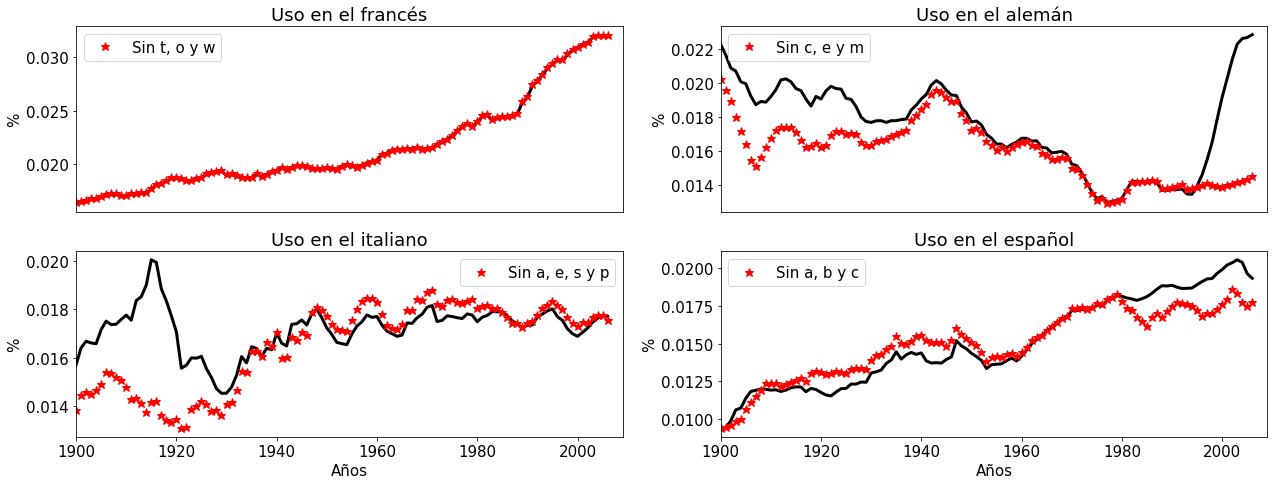
\includegraphics[scale=.375]{Cap_5/OM_EN.png}
	\label{fig.OM_EN}
	\caption{Omisiones del inglés en los demás}
\end{figure}



\newpage
\subsection{Francés}

\begin{figure}[h!]
	\centering
	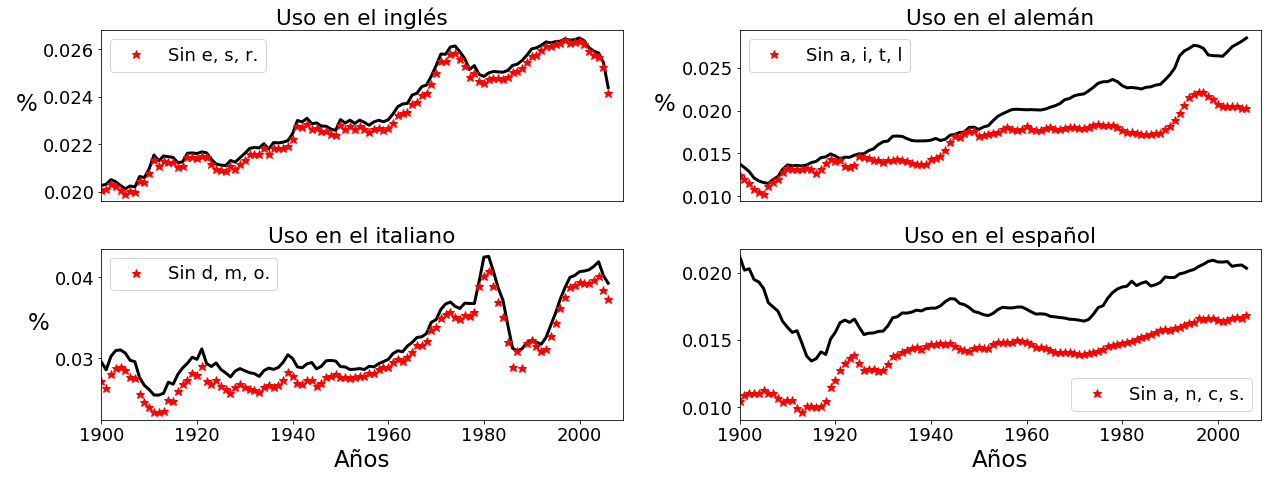
\includegraphics[scale=.375]{Cap_5/OM_FR.png}
	\label{fig.OM_FR}
	\caption{Omisiones del francés en los demás}
\end{figure}


\newpage
\subsection{Alemán}

\begin{figure}[h!]
	\centering
	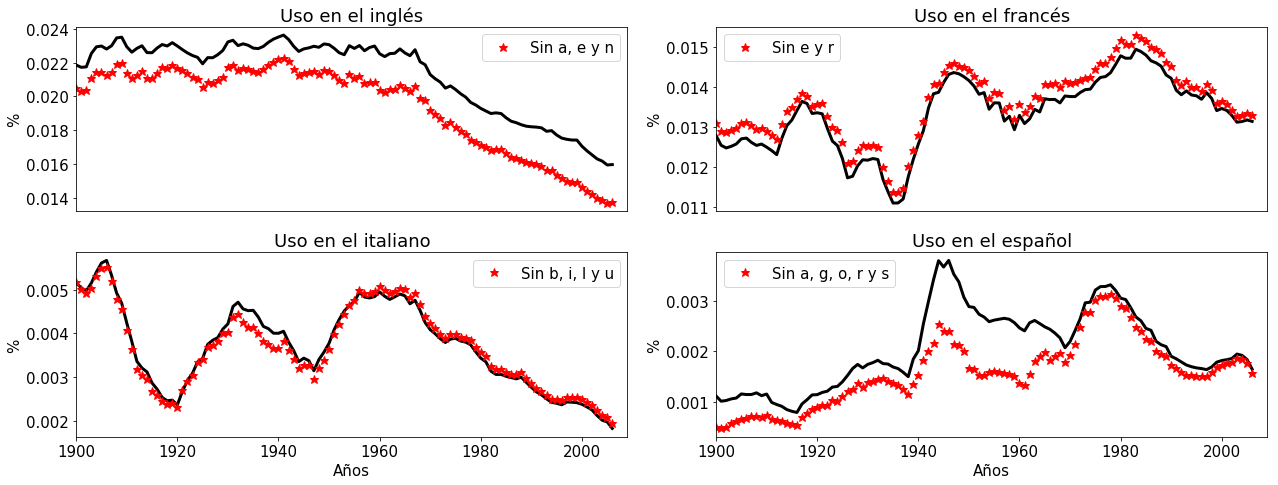
\includegraphics[scale=.375]{Cap_5/OM_GE.png}
	\label{fig.OM_GE}
	\caption{Omisiones del alemán en los demás}
\end{figure}


\newpage
\subsection{Italiano}

\begin{figure}[h!]
	\centering
	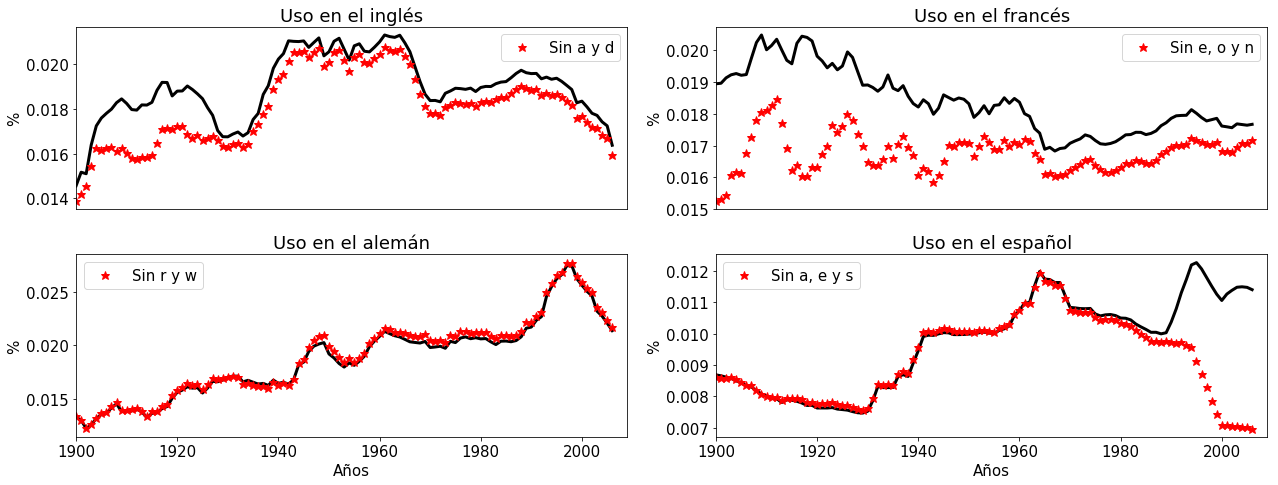
\includegraphics[scale=.375]{Cap_5/OM_IT.png}
	\label{fig.OM_IT}
	\caption{Omisiones del italiano en los demás}
\end{figure}


\newpage
\subsection{Español}

\begin{figure}[h!]
	\centering
	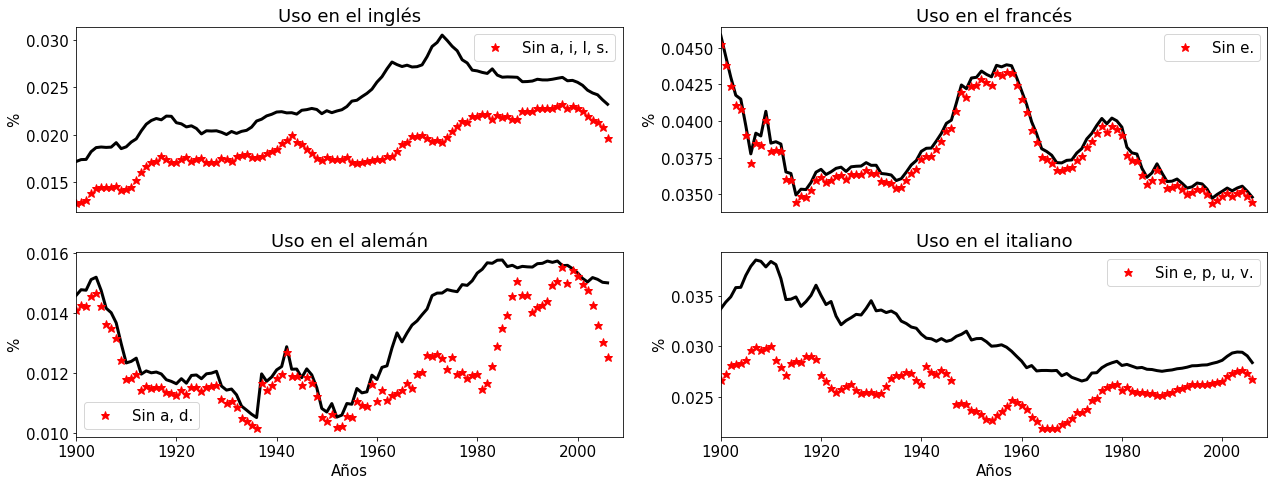
\includegraphics[scale=.375]{Cap_5/OM_SP.png}
	\label{fig.OM_SP}
	\caption{Omisiones del español en los demás}
\end{figure}
            % ~5 páginas - Resumir lo que se hizo y lo que no y comentar trabajos futuros sobre el tema
\chapter{Conclusiones} 
%%%%%%%%%%%%%%%%%%%%%%%%%%%%%%%%%%%%%%%%%%%%%%%%%%%%%
%                   APÉNDICES                       %
%%%%%%%%%%%%%%%%%%%%%%%%%%%%%%%%%%%%%%%%%%%%%%%%%%%%%
\appendix
% this file is called up by thesis.tex
% content in this file will be fed into the main document
\chapter{Complementos}
% top level followed by section, subsection

\section{Lectura de listas}

\newpage

\section{Gráficas de palabras nuevas entre dos idiomas}

\begin{figure}[h!]
	\centering
	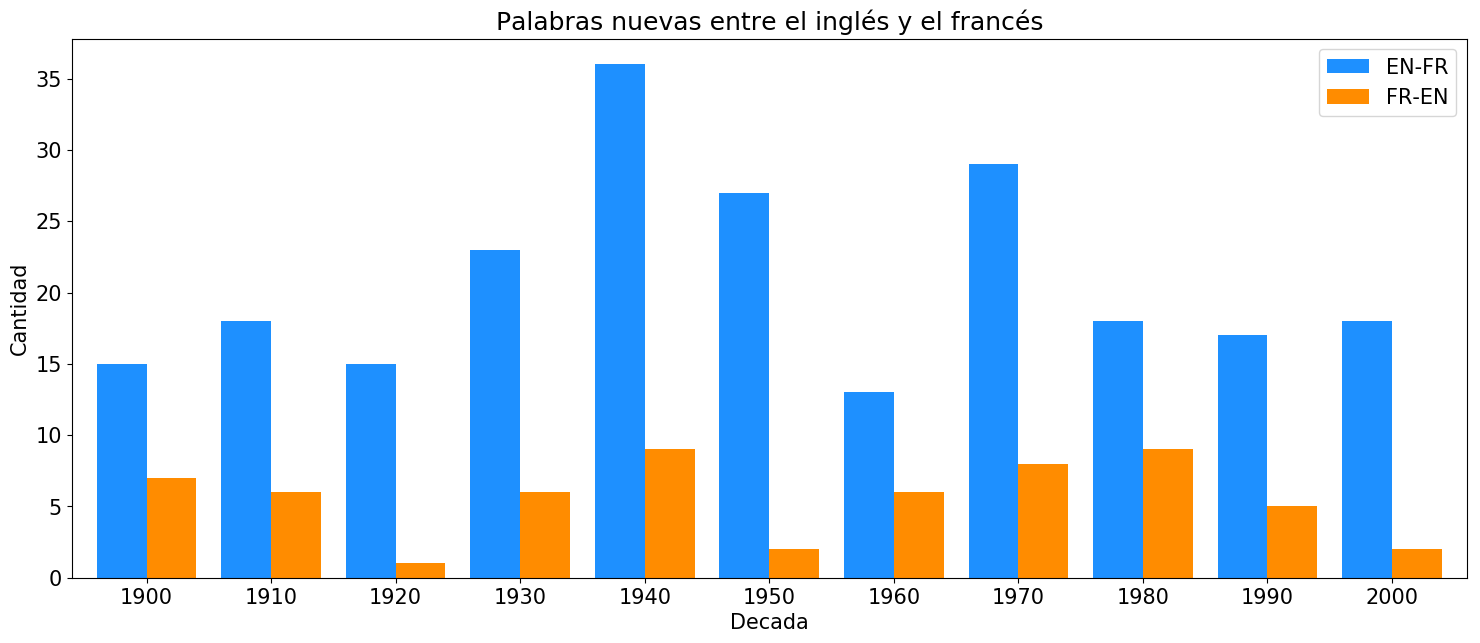
\includegraphics[scale=.38]{Cap_3/NC_1_S2_EN.png}
	\label{fig.NC_EF}
	\caption{Palabras nuevas entre el inglés y el francés}
\end{figure}

\begin{figure}[h!]
	\centering
	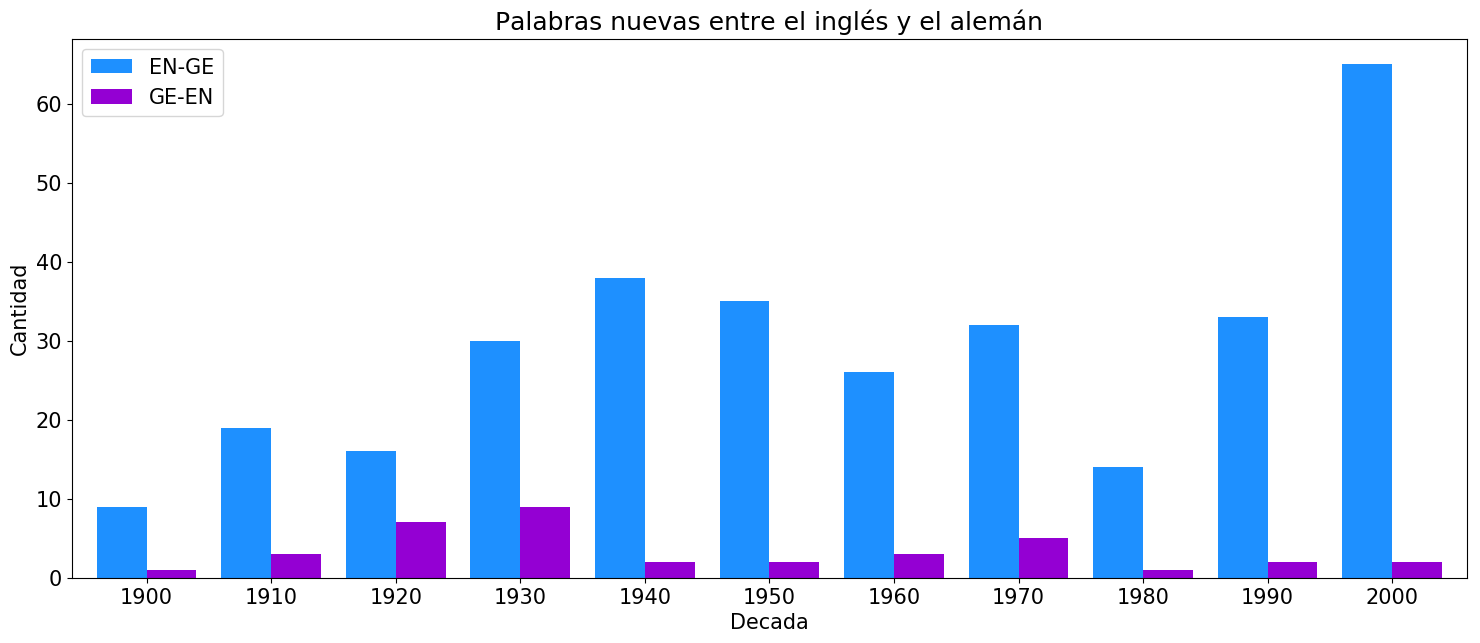
\includegraphics[scale=.38]{Cap_3/NC_2_S2_EN.png}
	\label{fig.NC_EG}
	\caption{Palabras nuevas entre el inglés y el alemán}
\end{figure}

\begin{figure}[h!]
	\centering
	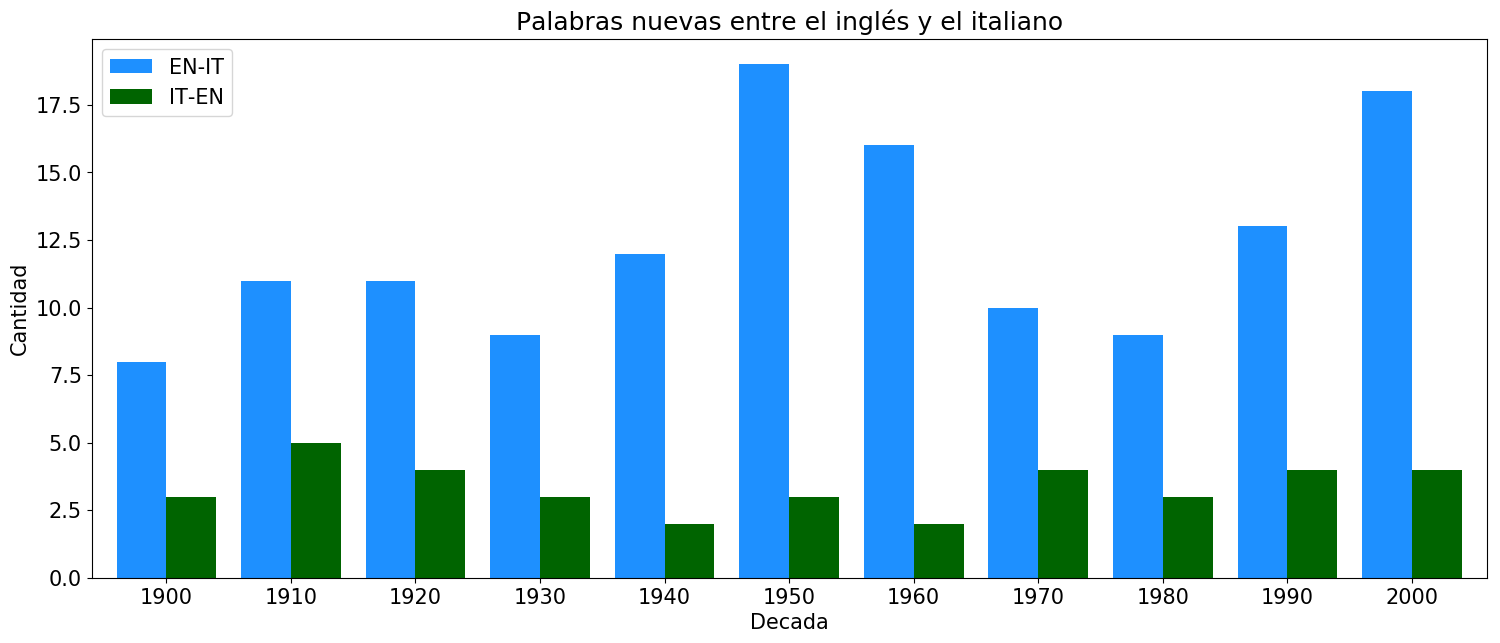
\includegraphics[scale=.38]{Cap_3/NC_3_S2_EN.png}
	\label{fig.NC_EI}
	\caption{Palabras nuevas entre el inglés y el italiano}
\end{figure}


\begin{figure}[h!]
	\centering
	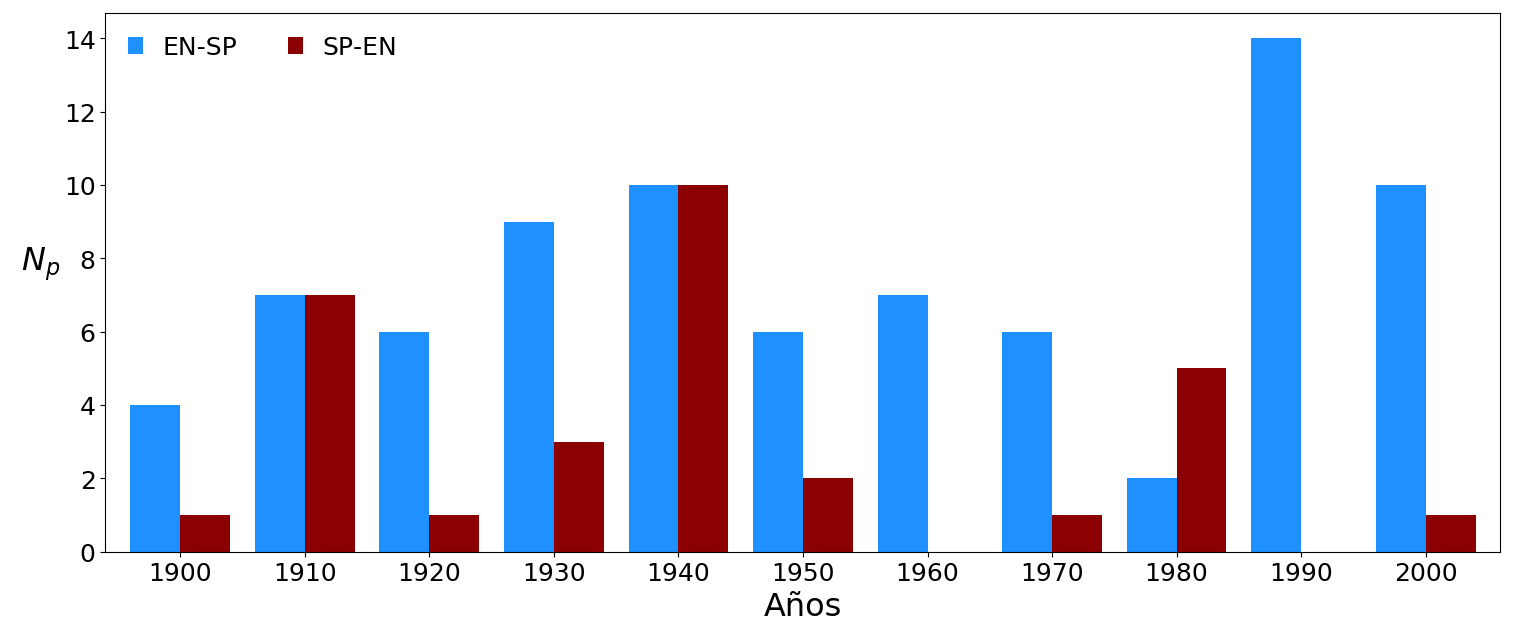
\includegraphics[scale=.38]{Cap_3/NC_4_S2_EN.png}
	\label{fig.NC_ES}
	\caption{Palabras nuevas entre el inglés y el español}
\end{figure}

\begin{figure}[h!]
	\centering
	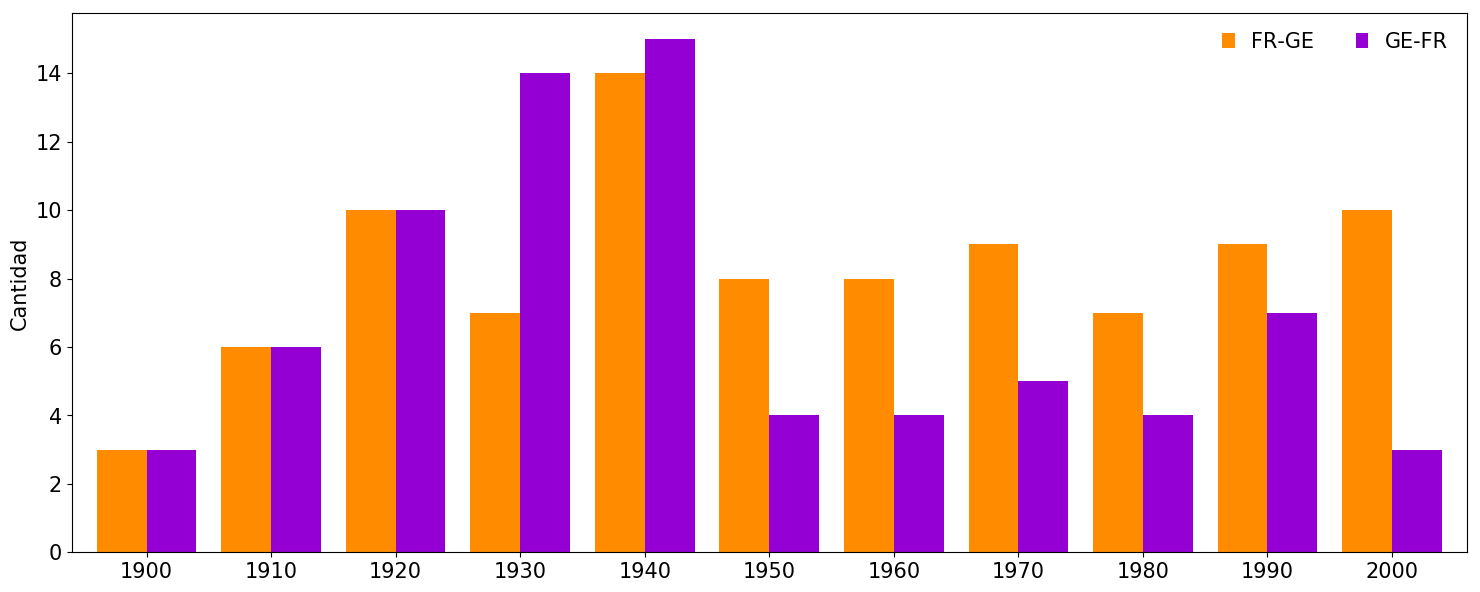
\includegraphics[scale=.38]{Cap_3/NC_2_S2_FR.png}
	\label{fig.NC_FG}
	\caption{Palabras nuevas entre el francés y el alemán}
\end{figure}


\begin{figure}[h!]
	\centering
	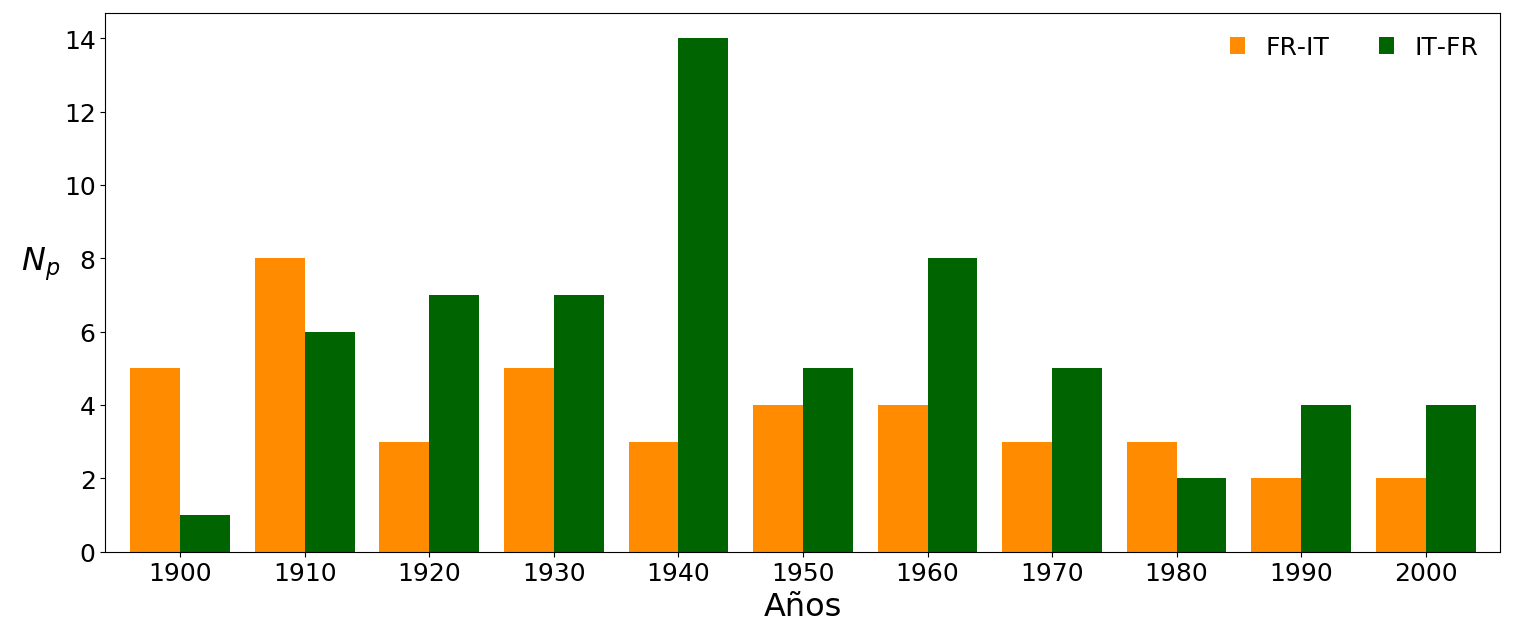
\includegraphics[scale=.38]{Cap_3/NC_3_S2_FR.png}
	\label{fig.NC_FI}
	\caption{Palabras nuevas entre el francés y el italiano}
\end{figure}

\begin{figure}[h!]
	\centering
	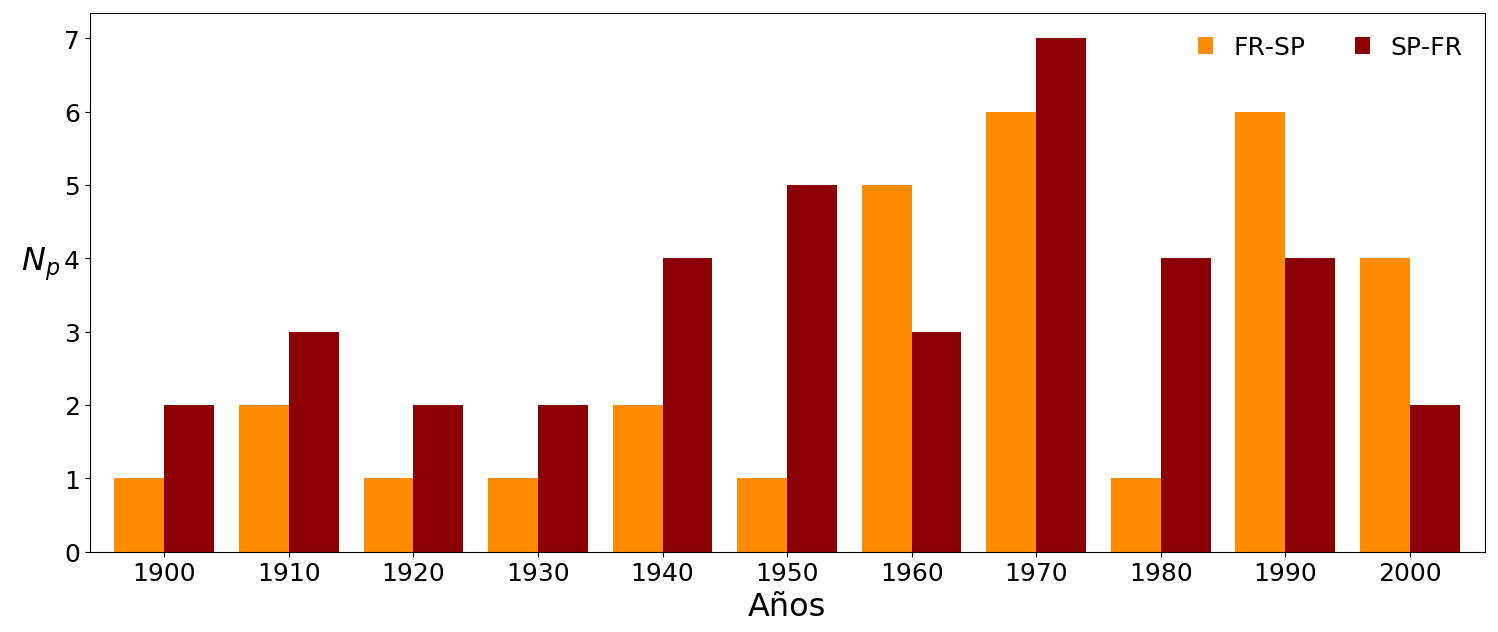
\includegraphics[scale=.38]{Cap_3/NC_4_S2_FR.png}
	\label{fig.NC_FS}
	\caption{Palabras nuevas entre el francés y el español}
\end{figure}

\begin{figure}[h!]
	\centering
	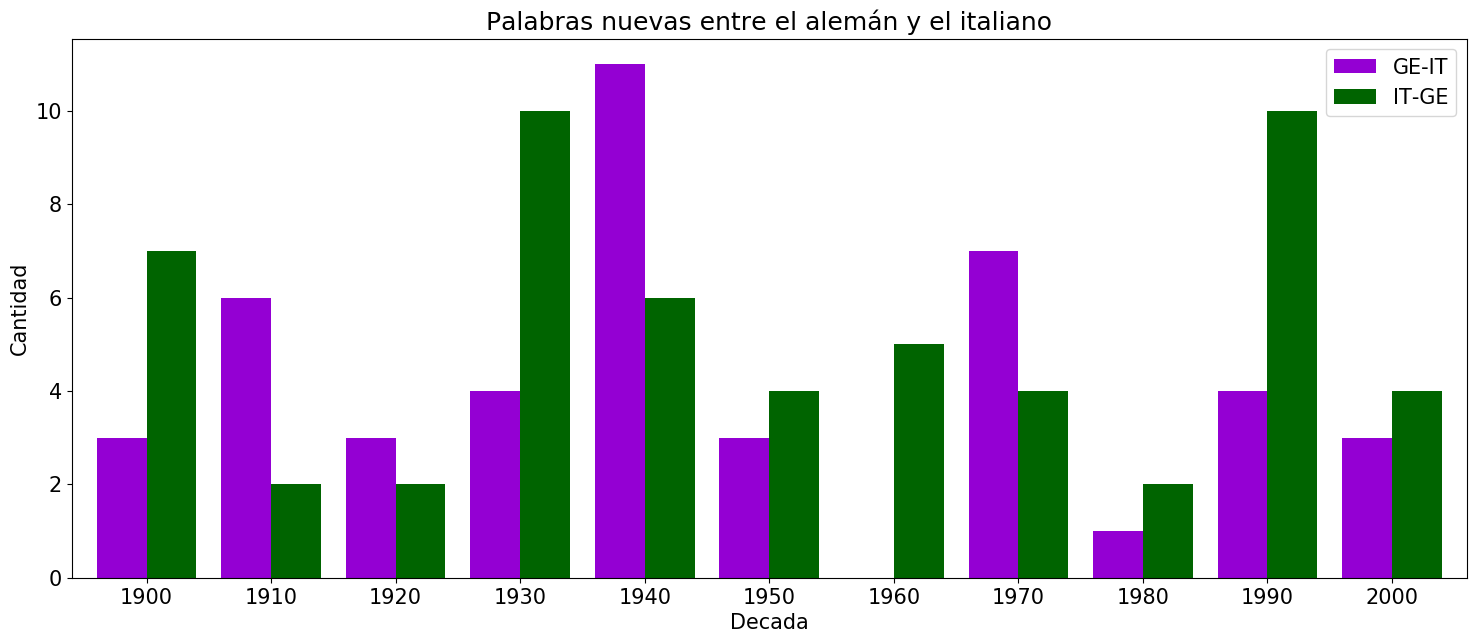
\includegraphics[scale=.38]{Cap_3/NC_3_S2_GE.png}
	\label{fig.NC_GI}
	\caption{Palabras nuevas entre el alemán y el italiano}
\end{figure}

\begin{figure}[h!]
	\centering
	\includegraphics[scale=.38]{Cap_3/NC_4_S2_GE.png}
	\label{fig.NC_GS}
	\caption{Palabras nuevas entre el alemán y el español}
\end{figure}

\begin{figure}[h!]
	\centering
	\includegraphics[scale=.38]{Cap_3/NC_4_S2_IT.png}
	\label{fig.NC_IS}
	\caption{Palabras nuevas entre el italiano y el español}
\end{figure}

\newpage


\section{Gráficas de palabras acumuladas entre dos idiomas}

\begin{figure}[h!]
	\centering
	\includegraphics[scale=.38]{Cap_4/SF_1_S2_EN.png}
	\label{fig.SF_EF}
	\caption{Palabras acumuladas entre el inglés y el francés}
\end{figure}


\begin{figure}[h!]
	\centering
	\includegraphics[scale=.38]{Cap_4/SF_2_S2_EN.png}
	\label{fig.SF_EG}
	\caption{Palabras acumuladas entre el inglés y el alemán}
\end{figure}


\begin{figure}[h!]
	\centering
	\includegraphics[scale=.38]{Cap_4/SF_3_S2_EN.png}
	\label{fig.SF_EI}
	\caption{Palabras acumuladas entre el inglés y el italiano}
\end{figure}

\begin{figure}[h!]
	\centering
	\includegraphics[scale=.38]{Cap_4/SF_4_S2_EN.png}
	\label{fig.SF_ES}
	\caption{Palabras acumuladas entre el inglés y el español}
\end{figure}

\begin{figure}[h!]
	\centering
	\includegraphics[scale=.38]{Cap_4/SF_2_S2_FR.png}
	\label{fig.SF_FG}
	\caption{Palabras acumuladas entre el francés y el alemán}
\end{figure}

\begin{figure}[h!]
	\centering
	\includegraphics[scale=.38]{Cap_4/SF_3_S2_FR.png}
	\label{fig.SF_FI}
	\caption{Palabras acumuladas entre el francés y el italiano}
\end{figure}

\begin{figure}[h!]
	\centering
	\includegraphics[scale=.38]{Cap_4/SF_4_S2_FR.png}
	\label{fig.SF_FS}
	\caption{Palabras acumuladas entre el francés y el español}
\end{figure}



\begin{figure}[h!]
	\centering
	\includegraphics[scale=.38]{Cap_4/SF_3_S2_GE.png}
	\label{fig.SF_GI}
	\caption{Palabras acumuladas entre el alemán y el italiano}
\end{figure}


\begin{figure}[h!]
	\centering
	\includegraphics[scale=.38]{Cap_4/SF_4_S2_GE.png}
	\label{fig.SF_GS}
	\caption{Palabras acumuladas entre el alemán y el español}
\end{figure}


\begin{figure}[h!]
	\centering
	\includegraphics[scale=.38]{Cap_4/SF_4_S2_IT.png}
	\label{fig.SF_IE}
	\caption{Palabras acumuladas entre el italiano y el español}
\end{figure}
               % Colocar los circuitos, manuales, código fuente, pruebas de teoremas, etc.

%%%%%%%%%%%%%%%%%%%%%%%%%%%%%%%%%%%%%%%%%%%%%%%%%%%%%
%                   REFERENCIAS                     %
%%%%%%%%%%%%%%%%%%%%%%%%%%%%%%%%%%%%%%%%%%%%%%%%%%%%%
% existen varios estilos de bilbiografía, pueden cambiarlos a placer
%\bibliographystyle{apalike} % otros estilos pueden ser abbrv, acm, alpha, apalike, ieeetr, plain, siam, unsrt

%El formato trae otros estilos, o pueden agregar uno que les guste:
%\bibliographystyle{Latex/Classes/PhDbiblio-case} % title forced lower case
%\bibliographystyle{Latex/Classes/PhDbiblio-bold} % title as in bibtex but bold
\bibliographystyle{Latex/Classes/PhDbiblio-url} % bold + www link if provided
%\bibliographystyle{Latex/Classes/jmb} % calls style file jmb.bst

\bibliography{Bibliografia/referencias}             % Archivo .bib


\end{document}
